\documentclass[specialist,
substylefile = spbu_report.rtx,
subf,href,colorlinks=true, 12pt]{disser}
\usepackage[utf8]{inputenc}
\usepackage[english,russian]{babel}

\usepackage[a4paper,
mag=1000, includefoot,
left=3cm, right=1.5cm, top=2cm, bottom=2cm, headsep=1cm, footskip=1cm]{geometry}

\usepackage{graphicx,subcaption,ragged2e}

\usepackage{amsthm}
\usepackage{amsmath}
\usepackage{amssymb}

\usepackage{hhline}

\usepackage{xcolor}

\usepackage{array}

\usepackage{bbm}

\theoremstyle{definition}
\newtheorem{definition}{Определение}
\newtheorem{algorithm}{Алгоритм}
\newtheorem{remark}{Замечание}
\newtheorem{example}{Пример}

\newcommand{\R}{\mathbb{R}}

\newcommand{\bfxi}{\boldsymbol{\xi}}

%new calligraphic font for subspaces 
\usepackage{euscript}
\newcommand{\cA}{\EuScript{A}}
\newcommand{\cB}{\EuScript{B}}
\newcommand{\cC}{\EuScript{C}}
\newcommand{\cD}{\EuScript{D}}
\newcommand{\cE}{\EuScript{E}}
\newcommand{\cF}{\EuScript{F}}
\newcommand{\cG}{\EuScript{G}}
\newcommand{\cH}{\EuScript{H}}
\newcommand{\cI}{\EuScript{I}}
\newcommand{\cJ}{\EuScript{J}}
\newcommand{\cK}{\EuScript{K}}
\newcommand{\cL}{\EuScript{L}}
\newcommand{\cM}{\EuScript{M}}
\newcommand{\cN}{\EuScript{N}}
\newcommand{\cO}{\EuScript{O}}
\newcommand{\cP}{\EuScript{P}}
\newcommand{\cQ}{\EuScript{Q}}
\newcommand{\cR}{\EuScript{R}}
\newcommand{\cS}{\EuScript{S}}
\newcommand{\cT}{\EuScript{T}}
\newcommand{\cU}{\EuScript{U}}
\newcommand{\cV}{\EuScript{V}}
\newcommand{\cW}{\EuScript{W}}
\newcommand{\cX}{\EuScript{X}}
\newcommand{\cY}{\EuScript{Y}}
\newcommand{\cZ}{\EuScript{Z}}

%font for text indices like transposition X^\mathrm{T}
\newcommand{\rmA}{\mathrm{A}}
\newcommand{\rmB}{\mathrm{B}}
\newcommand{\rmC}{\mathrm{C}}
\newcommand{\rmD}{\mathrm{D}}
\newcommand{\rmE}{\mathrm{E}}
\newcommand{\rmF}{\mathrm{F}}
\newcommand{\rmG}{\mathrm{G}}
\newcommand{\rmH}{\mathrm{H}}
\newcommand{\rmI}{\mathrm{I}}
\newcommand{\rmJ}{\mathrm{J}}
\newcommand{\rmK}{\mathrm{K}}
\newcommand{\rmL}{\mathrm{L}}
\newcommand{\rmM}{\mathrm{M}}
\newcommand{\rmN}{\mathrm{N}}
\newcommand{\rmO}{\mathrm{O}}
\newcommand{\rmP}{\mathrm{P}}
\newcommand{\rmQ}{\mathrm{Q}}
\newcommand{\rmR}{\mathrm{R}}
\newcommand{\rmS}{\mathrm{S}}
\newcommand{\rmT}{\mathrm{T}}
\newcommand{\rmU}{\mathrm{U}}
\newcommand{\rmV}{\mathrm{V}}
\newcommand{\rmW}{\mathrm{W}}
\newcommand{\rmX}{\mathrm{X}}
\newcommand{\rmY}{\mathrm{Y}}
\newcommand{\rmZ}{\mathrm{Z}}

%tt font for time series
\newcommand{\tA}{\mathsf{A}}
\newcommand{\tB}{\mathsf{B}}
\newcommand{\tC}{\mathsf{C}}
\newcommand{\tD}{\mathsf{D}}
\newcommand{\tE}{\mathsf{E}}
\newcommand{\tF}{\mathsf{F}}
\newcommand{\tG}{\mathsf{G}}
\newcommand{\tH}{\mathsf{H}}
\newcommand{\tI}{\mathsf{I}}
\newcommand{\tJ}{\mathsf{J}}
\newcommand{\tK}{\mathsf{K}}
\newcommand{\tL}{\mathsf{L}}
\newcommand{\tM}{\mathsf{M}}
\newcommand{\tN}{\mathsf{N}}
\newcommand{\tO}{\mathsf{O}}
\newcommand{\tP}{\mathsf{P}}
\newcommand{\tQ}{\mathsf{Q}}
\newcommand{\tR}{\mathsf{R}}
\newcommand{\tS}{\mathsf{S}}
\newcommand{\tT}{\mathsf{T}}
\newcommand{\tU}{\mathsf{U}}
\newcommand{\tV}{\mathsf{V}}
\newcommand{\tW}{\mathsf{W}}
\newcommand{\tX}{\mathsf{X}}
\newcommand{\tY}{\mathsf{Y}}
\newcommand{\tZ}{\mathsf{Z}}

%bf font for matrices
\newcommand{\bfA}{\mathbf{A}}
\newcommand{\bfB}{\mathbf{B}}
\newcommand{\bfC}{\mathbf{C}}
\newcommand{\bfD}{\mathbf{D}}
\newcommand{\bfE}{\mathbf{E}}
\newcommand{\bfF}{\mathbf{F}}
\newcommand{\bfG}{\mathbf{G}}
\newcommand{\bfH}{\mathbf{H}}
\newcommand{\bfI}{\mathbf{I}}
\newcommand{\bfJ}{\mathbf{J}}
\newcommand{\bfK}{\mathbf{K}}
\newcommand{\bfL}{\mathbf{L}}
\newcommand{\bfM}{\mathbf{M}}
\newcommand{\bfN}{\mathbf{N}}
\newcommand{\bfO}{\mathbf{O}}
\newcommand{\bfP}{\mathbf{P}}
\newcommand{\bfQ}{\mathbf{Q}}
\newcommand{\bfR}{\mathbf{R}}
\newcommand{\bfS}{\mathbf{S}}
\newcommand{\bfT}{\mathbf{T}}
\newcommand{\bfU}{\mathbf{U}}
\newcommand{\bfV}{\mathbf{V}}
\newcommand{\bfW}{\mathbf{W}}
\newcommand{\bfX}{\mathbf{X}}
\newcommand{\bfY}{\mathbf{Y}}
\newcommand{\bfZ}{\mathbf{Z}}

%bb font for standard spaces and expectation
\newcommand{\bbA}{\mathbb{A}}
\newcommand{\bbB}{\mathbb{B}}
\newcommand{\bbC}{\mathbb{C}}
\newcommand{\bbD}{\mathbb{D}}
\newcommand{\bbE}{\mathbb{E}}
\newcommand{\bbF}{\mathbb{F}}
\newcommand{\bbG}{\mathbb{G}}
\newcommand{\bbH}{\mathbb{H}}
\newcommand{\bbI}{\mathbb{I}}
\newcommand{\bbJ}{\mathbb{J}}
\newcommand{\bbK}{\mathbb{K}}
\newcommand{\bbL}{\mathbb{L}}
\newcommand{\bbM}{\mathbb{M}}
\newcommand{\bbN}{\mathbb{N}}
\newcommand{\bbO}{\mathbb{O}}
\newcommand{\bbP}{\mathbb{P}}
\newcommand{\bbQ}{\mathbb{Q}}
\newcommand{\bbR}{\mathbb{R}}
\newcommand{\bbS}{\mathbb{S}}
\newcommand{\bbT}{\mathbb{T}}
\newcommand{\bbU}{\mathbb{U}}
\newcommand{\bbV}{\mathbb{V}}
\newcommand{\bbW}{\mathbb{W}}
\newcommand{\bbX}{\mathbb{X}}
\newcommand{\bbY}{\mathbb{Y}}
\newcommand{\bbZ}{\mathbb{Z}}

%got font for any case
\newcommand{\gA}{\mathfrak{A}}
\newcommand{\gB}{\mathfrak{B}}
\newcommand{\gC}{\mathfrak{C}}
\newcommand{\gD}{\mathfrak{D}}
\newcommand{\gE}{\mathfrak{E}}
\newcommand{\gF}{\mathfrak{F}}
\newcommand{\gG}{\mathfrak{G}}
\newcommand{\gH}{\mathfrak{H}}
\newcommand{\gI}{\mathfrak{I}}
\newcommand{\gJ}{\mathfrak{J}}
\newcommand{\gK}{\mathfrak{K}}
\newcommand{\gL}{\mathfrak{L}}
\newcommand{\gM}{\mathfrak{M}}
\newcommand{\gN}{\mathfrak{N}}
\newcommand{\gO}{\mathfrak{O}}
\newcommand{\gP}{\mathfrak{P}}
\newcommand{\gQ}{\mathfrak{Q}}
\newcommand{\gR}{\mathfrak{R}}
\newcommand{\gS}{\mathfrak{S}}
\newcommand{\gT}{\mathfrak{T}}
\newcommand{\gU}{\mathfrak{U}}
\newcommand{\gV}{\mathfrak{V}}
\newcommand{\gW}{\mathfrak{W}}
\newcommand{\gX}{\mathfrak{X}}
\newcommand{\gY}{\mathfrak{Y}}
\newcommand{\gZ}{\mathfrak{Z}}

%old calligraphic font
\newcommand{\calA}{\mathcal{A}}
\newcommand{\calB}{\mathcal{B}}
\newcommand{\calC}{\mathcal{C}}
\newcommand{\calD}{\mathcal{D}}
\newcommand{\calE}{\mathcal{E}}
\newcommand{\calF}{\mathcal{F}}
\newcommand{\calG}{\mathcal{G}}
\newcommand{\calH}{\mathcal{H}}
\newcommand{\calI}{\mathcal{I}}
\newcommand{\calJ}{\mathcal{J}}
\newcommand{\calK}{\mathcal{K}}
\newcommand{\calL}{\mathcal{L}}
\newcommand{\calM}{\mathcal{M}}
\newcommand{\calN}{\mathcal{N}}
\newcommand{\calO}{\mathcal{O}}
\newcommand{\calP}{\mathcal{P}}
\newcommand{\calQ}{\mathcal{Q}}
\newcommand{\calR}{\mathcal{R}}
\newcommand{\calS}{\mathcal{S}}
\newcommand{\calT}{\mathcal{T}}
\newcommand{\calU}{\mathcal{U}}
\newcommand{\calV}{\mathcal{V}}
\newcommand{\calW}{\mathcal{W}}
\newcommand{\calX}{\mathcal{X}}
\newcommand{\calY}{\mathcal{Y}}
\newcommand{\calZ}{\mathcal{Z}}


\begin{document}
\setcounter{tocdepth}{2}
%
% Титульный лист на русском языке
%
% Название организации
\institution{%
	Санкт-Петербургский государственный университет\\
	Прикладная математика и информатика
}

\title{Отчет по учебной практике 4 (научно-исследовательской работе) (семестр 8)}

% Тема
\topic{Метод Монте-Карло SSA для одномерных и многомерных временных рядов}

% Автор
\author{Потешкин Егор Павлович}
\group{группа 20.Б04-мм}

% Научный руководитель
\sa       {Голяндина Нина Эдуардовна \\%
	Кафедра Статистического Моделирования}
\sastatus {д.\,ф.-м.\,н., доцент}

% Город и год
\city{Санкт-Петербург}
\date{\number\year}

\maketitle
\tableofcontents
\intro
Метод Singular Spectrum Analysis (SSA) является мощным инструментом для анализа временных рядов. Он позволяет разложить ряд на интерпретируемые компоненты, такие как тренд, периодические колебания и шум, что значительно упрощает процесс анализа. Метод Monte-Carlo SSA, в свою очередь, решает задачу обнаружения сигнала в шуме~\cite{Golyandina_2023}.

Однако, вариант Monte-Carlo SSA для анализа многомерных временных рядов мало исследован. В работе~\cite{Larin_2022} рассматривается применение метода Monte Carlo SSA для анализа многомерных временных рядов, и авторы сталкиваются с проблемой отсутствия реализации Тёплицева варианта MSSA в пакете Rssa~\cite{Rssa}.

В этой работе была поставлена задача реализовать двумя способами метод Toeplitz MSSA, сравнить их между собой и с обычным MSSA как для методов оценки сигнала, так и для использования в Monte-Carlo MSSA, а также рассмотреть Monte-Carlo SSA в условиях реальных задач.

В главе~\ref{chpt:mssa} приведено описание метода MSSA и двух его модификаций, и их численное сравнение. В главе~\ref{chpt:mc-ssa} представлен метод Monte-Carlo SSA, и приведено численное сравнение метода с разными параметрами. В ходе работы в этом семестре была добавлена глава~\ref{chpt:mc_ssa_real}, в которой рассмотрено два способа оценки неизвестных параметров красного шума и их сравнение, а также разобран случай Monte-Carlo SSA, когда во временном ряде присутствует мешающий сигнал. 

Впервые Monte-Carlo SSA упоминается в~\cite{Allen}, алгоритм которого совпадает одиночным тестом MC-SSA, представленным в этой работе. В~\cite{NAO} метод был применен на данных о зимнем индексе Североатлантического колебания (NAO index), и были обнаружены значимые колебания с периодом $7.7$ лет. В~\cite{Enchanced_mcssa} повторили результат работы~\cite{NAO} уже на ежемесячном индексе Североатлантического колебания: с помощью усовершенствованного Monte-Carlo SSA (enhanced MC-SSA) был обнаружен сигнал с периодом в $7.8$ лет. В~\cite{non_lin_ssa} представлен нелинейный вариант Monte-Carlo SSA, использующий ядерный анализ главных компонент (kernel PCA). В работе~\cite{gps} метод применяется для извлечения сезонных колебаний из непрерывных GPS-наблюдений, однако отмечается, что модель AR(1) может быть неподходящей для этих данных.
%Рассмотрим вещественнозначный временной ряд, т.е. последовательность вещественнозначных чисел, упорядоченных по времени. Метод Singular Spectrum Analysis (SSA) позволяет представить такой ряд в виде суммы интерпретируемых компонент, таких как тренд, периодические компоненты и шум, что упрощает процесс анализа временного ряда.

%В повседневной жизни чаще всего временные ряды встречаются в виде детерминированного сигнала и случайного шума. Тогда возникает задача обнаружения сигнала в шуме. Метод Monte-Carlo SSA "--- решение этой задачи.  

%Существует вариант Monte-Carlo SSA для анализа многомерных временных рядов, однако этот вариант мало исследован. В работе~\cite{Larin_2022} были численно исследованы свойства метода Monte-Carlo SSA, однако исследование не было завершено полностью, возникла проблема необходимости реализации Тёплицева варианта Multivariate SSA (MSSA), но ее не было в используемом пакете Rssa~\cite{Rssa}.

%Целью данной работы является реализация метода Тёплицева MSSA двумя способами, а также сравнение способов между собой и с базовой версией MSSA. Было произведено сравнение точности методов в восстановлении сигнала и в использовании в Monte-Carlo MSSA.  

\chapter{Метод MSSA и его модификации}\label{chpt:mssa}
В этой главе рассматривается метод Multivariate Singular Spectrum Analysis~\cite{Golyandina_2015} (сокращенно MSSA) и его модификации. В разделе~\ref{sect:definitions} представлены вспомогательные определения, нужные в дальнейшем. В разделе~\ref{sect:mssa} представлен алгоритм метода MSSA, а в разделах~\ref{sect:basic_mssa} и~\ref{sect:block} "--- его базовый и стандартный теплицев~\cite{Plaut1994SpellsOL} варианты. В разделе~\ref{sect:sum} предлагается другая теплицева модификация MSSA, и в разделе~\ref{sect:mssa_comparison} происходит сравнение методов MSSA: как теоретическое, так и численное.

\section{Вспомогательные определения}\label{sect:definitions}
\begin{definition}
	Пусть $\tX$ "--- одномерный временной ряд длины $N$. Выберем параметр $L$, называемый \emph{длиной окна}, $1<L<N$. Рассмотрим $K=N-L+1$ векторов вложения $X_i=(x_{i},\ldots, x_{i+L-1})^\rmT,\ 1\leqslant j \leqslant K$. Определим оператор вложения $\cT$ следующим образом:
	\begin{equation}\label{eq:embedding}
		\cT(\tX)=\bfX=[X_1:\ldots:X_K]=
		\begin{pmatrix}
			x_1    & x_2     & \cdots & x_K     \\
			x_2    & x_3     & \cdots & x_{K+1} \\
			\vdots & \vdots  & \ddots & \vdots  \\
			x_L    & x_{L+1} & \cdots & x_N
		\end{pmatrix}.
	\end{equation}
\end{definition}
\begin{definition}
	Матрицу $\bfX$ из~\eqref{eq:embedding} называют траекторной матрицей.
\end{definition}\noindent
Заметим, что матрица $\bfX$ является \emph{ганкелевой}, т.е на всех ее побочных диагоналях стоят одинаковые элементы, а оператор $\cT$ задает взаимно-однозначное соответствие между множеством временных рядов длины $N$ и множеством ганкелевых матриц $L\times K$.
\begin{definition}
	Пусть $\bfY=\{y_{ij}\}_{i,j=1}^{L,K}$ "--- некоторая матрица. Определим оператор ганкелизации $\cH$:
	\begin{equation}\label{eq:averaging}
		(\cH(\bfY))_{ij}=\sum_{(l,k)\in A_s}y_{lk}/w_s,
	\end{equation}
	где $s=i+j-1$, $A_s=\{(l,k)\, :\, l+k=s+1,\, 1\leqslant l\leqslant L,\, 1\leqslant k\leqslant K\}$ и $w_s=|A_s|$ "--- количество элементов в множестве $A_s$. Это соответствует
	усреднению элементов матрицы $\bfY$ по побочным диагоналям.
\end{definition}
\begin{definition}
	Случайный процесс $\xi=(\xi_1,\ldots, \xi_n,\ldots)$ называется стационарным, если $\forall k\geqslant1$ $\mathsf E\xi_k=\operatorname{const}$ и $\forall k,l\geqslant1$
	\[
	K(k, l)\overset{\text{def}}=\operatorname{cov}(\xi_k, \xi_l)= \widetilde{K}(k-l).
	\]
\end{definition}
\begin{definition}
	Белый гауссовский шум $\boldsymbol{\varepsilon}=(\varepsilon_1,\ldots,\varepsilon_n,\ldots)$ "--- стационарный случайный процес с $\varepsilon_n\sim N(0, \sigma^2)~\forall n$ и $\widetilde K(n)=0$, при $n>0$.
\end{definition}
\begin{definition}
	Детерминированный временной ряд $\tX=(x_1,\ldots,x_n,\ldots)$ называют стационарным, если существует функция $R_x(k)$ $(-\infty<k<+\infty)$ такая, что $\forall k,l\geqslant0$
	\begin{equation*}
		R_x^{(N)}(k,l)\overset{\text{def}}{=}\frac{1}{N}\sum_{m=1}^Nx_{k+m}x_{l+m}\underset{N\to\infty}\longrightarrow R_x(k - l).
	\end{equation*}
\end{definition}
\begin{definition}
	Рассмотрим вещественнозначные одномерные временные ряды $\tX^{(d)}$ длины $N_d$, $d=1,\ldots,D$. Тогда составленный из этих рядов $\tX=\{\tX^{(d)}\}_{d=1}^D$ "--- $D$-канальный временной ряд с длинами $N_d$.
\end{definition}
\begin{definition}
	Пусть $\tX=\{\tX^{(d)}\}_{d=1}^D$ "--- $D$-канальный временной ряд. Ряд $\tX$ называют стационарным, если каждый канал $\tX^{(d)}$ "--- стационарный.
\end{definition}

\section{Метод MSSA}\label{sect:mssa}
Метод MSSA состоит из четырех этапов: \emph{вложения}, \emph{разложения}, \emph{группировки} и \emph{диагонального усреднения}.

\subsection{Вложение}\label{sect:embedding}
Зафиксируем $L$, $1<L<\min(N_1,\ldots,N_D)$. Для каждого ряда $\tX^{(d)}$ составим траекторную матрицу $\bfX^{(d)}$ . Обозначим $K=\sum_{d=1}^D K_d$. Результатом этапа вложения является траекторная матрица многоканального временного ряда
\begin{equation}\label{eq:embedding_mssa}
	\bfX=\cT_{\text{MSSA}}(\tX)=[\cT(\tX^{(1)}):\ldots:\cT(\tX^{(D)})]=[\bfX^{(1)}:\ldots:\bfX^{(D)}].
\end{equation}
\subsection{Разложение}
Задача этапа разложения "--- разбить траекторную матрицу $\bfX$ в сумму матриц единичного ранга: $\bfX=\bfX_1+\ldots+\bfX_p$.
\begin{definition}
	Пусть $\bfX=\sum_i \sigma_i P_i Q_i^T$ "--- любое разложение $\bfX$ в сумму матриц ранга $1$. Будем называть $P_i$ \emph{левыми}, а $Q_i$ "--- \emph{правыми векторами} матрицы $\bfX$.
\end{definition}

\subsection{Группировка}\label{sect:grouping}
На этом шаге множество индексов $I=\{1,\ldots,p\}$ разбивается на $m$ непересекающихся множеств $I_1,\ldots,I_m$ и матрица $\bfX$ представляется в виде суммы
\[
	\bfX = \sum_{k=1}^m \bfX_{I_k},
\]
где $\bfX_{I_k}=\sum_{i\in I_k}\bfX_i$.

\subsection{Диагональное усреднение}\label{sect:averaging}
Пусть $\bfY=[\bfY^{(1)}:\ldots:\bfY^{(M)}]$ "--- некоторая составная матрица, тогда оператор ганкелизации для составной матрицы
\begin{equation}\label{eq:averaging_mssa}
\cH_{\text{stacked}}(\bfY)=[\cH(\bfY^{(1)}):\ldots:\cH(\bfY^{(M)})].
\end{equation}

Финальным шагом MSSA является преобразование каждой матрицы $\bfX_{I_k}$, составленной в разделе~\ref{sect:grouping}, в $D$-канальный временной ряд:
\begin{equation}
	\widetilde\tX_{I_k}=\cT_{\text{MSSA}}^{-1}\circ\cH_{\text{stacked}}\left(\bfX_{I_k}\right),
\end{equation}
где $\cT_{\text{MSSA}}$ "--- оператор вложения~\eqref{eq:embedding_mssa}, $\cH_{\text{stacked}}$ "--- оператор ганкелизации~\eqref{eq:averaging_mssa}.
\begin{remark}
При $D=1$ $\tX$ "--- одномерный временной ряд, и приведенный выше алгоритм совпадает с алгоритмом Basic SSA, описанный в~\cite{ssa_an}.
\end{remark}

\section{Этап разложения}\label{sect:decomposition}

Модификации MSSA отличаются только этапом разложения, остальные этапы остаются неизменными.
\subsection{Basic MSSA}\label{sect:basic_mssa}
Базовый вариант MSSA использует сингулярное разложение (SVD) матрицы $\bfX$. Положим $\mathbf{S}=\bfX\bfX^\rmT$. Пусть $\lambda_i$ "--- собственные числа, а $U_i$ "--- ортонормированная система векторов матрицы $\mathbf{S}$. Упорядочим $\lambda_i$ по убыванию и найдем $p$ такое, что $\lambda_p>0$, а $\lambda_{p+1}=0$. Тогда
\begin{equation}\label{eq:svd}
	\bfX=\sum_{i=1}^p\sqrt{\lambda_i}U_iV_i^\rmT=\sum_{i=1}^p\bfX_i,
\end{equation}
где $V_i=\bfX^\rmT U_i/\sqrt{\lambda_i}$. Тройку $(\sqrt{\lambda_i}, U_i, V_i)$ принято называть $i$-й собственной тройкой сингулярного разложения, $\sqrt{\lambda_i}$ "--- сингулярным числом, $U_i$ "--- левым сингулярным вектором, а $V_i$ "--- правым сингулярным вектором.

\begin{remark}\label{remark:svd}
	Левые сингулярные векторы $U_i$ являются собственными векторами матрицы $\bfX\bfX^\rmT$, а правые $V_i$ в свою очередь "--- матрицы $\bfX^\rmT\bfX$. В одномерном случае $U_i$ и $V_i$ равносильны с точностью до замены $L$ на $N-L+1$. Но при $D>1$ это не так по построению матрицы $\bfX$. Для наглядности рассмотрим случай $D=2$, тогда $\bfX\bfX^\rmT=\bfX^{(1)}(\bfX^{(1)})^\rmT + \bfX^{(2)}(\bfX^{(2)})^\rmT$, а
	\[
		\bfX^\rmT\bfX=
		\begin{pmatrix}
			(\bfX^{(1)})^\rmT\bfX^{(1)} & (\bfX^{(1)})^\rmT\bfX^{(2)} \\
			(\bfX^{(2)})^\rmT\bfX^{(1)} & (\bfX^{(2)})^\rmT\bfX^{(2)}
		\end{pmatrix}.
	\]
\end{remark}

\subsection{Toeplitz Block MSSA}\label{sect:block}
Если предполагается, что ряд $\tX$ стационарен, то можно заменить матрицу $\bfX\bfX^\rmT$ (или $\bfX^\rmT\bfX$ в силу замечания~\ref{remark:svd}) на некоторую другую, учитывая стационарность исходного ряда. Для этого введем следующее обозначение.
\begin{definition}
	Пусть $\tX=\{\tX^{(d)}\}_{d=1}^D$ "--- $D$-канальный временной ряд с $N_d=N$. Зафиксируем $1<M<N$. Обозначим за $\bfT_{l,k}^{(M)}\in \R^{M\times M}$ матрицу c элементами
	\begin{equation*}\label{eq:block_elements}
		\left(\bfT^{(M)}_{l,k}\right)_{ij}=\frac{1}{N-|i-j|}\sum_{n=1}^{N-|i-j|} x^{(l)}_nx^{(k)}_{n+|i-j|},\ 1\leqslant i,j\leqslant M,
	\end{equation*}
\end{definition}
\begin{remark}
	Если ряд $\tX$ стационарен, матрица $\bfT_{l,k}^{(M)}$ является оценкой кросс-ковариационной матрицы $l$ и $k$-го каналов.
\end{remark}
% \begin{remark}
% 	В отличие от матрицы $\bfC=\left(\bfX^{(l)}\right)^\rmT \bfX^{(k)}/L$, которая тоже является оценкой кросс-ковариационной матрицы, у матрицы $\bfT_{l,k}^{(K)}$ всего $K=N-L+1$ неизвестных параметров (у $\bfC$ их $K^2$). 
% \end{remark}
В работе~\cite{Plaut1994SpellsOL} предложен способ разложения $\bfX$, который мы назовем Toeplitz Block MSSA. Этот способ использует вместо матрицы $\bfX^\rmT\bfX$ матрицу $$\bfT_{\text{Block}}=\begin{pmatrix}
	\bfT^{(K)}_{1,1} & \bfT^{(K)}_{1,2} & \cdots & \bfT^{(K)}_{1,D} \\
	\bfT^{(K)}_{2,1} & \bfT^{(K)}_{2,2} & \cdots & \bfT^{(K)}_{2,D} \\
	\vdots           & \vdots           & \ddots & \vdots           \\
	\bfT^{(K)}_{D,1} & \bfT^{(K)}_{D,D} & \cdots & \bfT^{(K)}_{D,D}
\end{pmatrix} \in \R^{DK\times DK},$$ где $K = N - L + 1$. Найдя ортонормированные собственные векторы $Q_1,\ldots,Q_{DK}$ матрицы $\bfT_\text{Block}$, получаем разложение траекторной матрицы $\bfX$:
\begin{equation}\label{eq:block_decomposition}
	\mathbf{X}=\sum_{i=1}^{DK} \sigma_i P_i Q_i^\rmT=\bfX_1+\ldots+\bfX_{DK},
\end{equation}
где $Z_i=\bfX Q_i$, $P_i=Z_i/\|Z_i\|$, $\sigma_i=\|Z_i\|$.

\subsection{Toeplitz Sum MSSA}\label{sect:sum}
Вместе с методом Block рассмотрим другой вариант разложения, который назовем Sum. Рассмотрим вместо матрицы $\bfX\bfX^\rmT$ матрицу $\bfT_{\text{Sum}}=\sum_{d=1}^D \bfT_{d,d}^{(L)}\in\R^{L\times L}$. Найдем ортонормированные собственные векторы $P_1,\ldots,P_L$ матрицы $\bfT_{\text{Sum}}$ и разложим траекторную матрицу $\bfX$ следующим образом:
\begin{equation}\label{eq:sum_decomposition}
	\mathbf{X}=\sum_{i=1}^L\sigma_i P_iQ_i^\rmT=\bfX_1+\ldots+\bfX_L,
\end{equation}
где $S_i=\bfX^\rmT P_i$, $Q_i=S_i/\|S_i\|$, $\sigma_i=\|S_i\|$.

\section{Сравнение методов MSSA}\label{sect:mssa_comparison}
\subsection{Теоретическое сравнение методов}
Базовый вариант MSSA можно использовать для временных рядов с разными длинами каналов. Toeplitz Sum MSSA также позволяет это делать, в отличие от Toeplitz Block MSSA. Связано это с вычислением матриц $\bfT_{l,k}^{(K)}$, для которых при $l\ne k$ обязательно условие $N_l=N_k$. В методе Sum такой проблемы не возникает, поскольку $l=k$ всегда.

Также имеет смысл сравнить обе модификации по трудоемкости построения матриц и нахождения их собственных векторов. В методе Block нужно построить $D(D+1)/2$ теплицевых матриц размера $K\times K$, в методе Sum "--- $D$ теплицевых матриц размера $L\times L$. Тогда, учитывая, что для матрица $\bfT_{l,k}^{(M)}$ задается $M$ элементами, метод Sum численно эффективнее метода Block в построении матрицы, когда выполняется неравенство
\begin{equation*}
	\frac{D(D+1)K}2 > DL \iff (D+1)N - (D+1)L + (D+1) > 2L \iff L < \frac{(D+1)(N+1)}{D+3}.
\end{equation*}
Что касается нахождения собственных векторов, если использовать спектральное разложение матрицы, то трудоемкость составляет $\mathcal{O}(D^3K^3)$ для метода Block и $\mathcal{O}(L^3)$ для метода Sum.

\subsection{Численное сравнение методов}
Посмотрим на точность базового и модифицированных методов MSSA для разных значений параметра $L$. Рассмотрим следующий двухканальный временной ряд длины ${N=71}$:
$$\{\tF^{(1)}, \tF^{(2)}\}=\{\tS^{(1)},\tS^{(2)}\} + \{\tN^{(1)},\tN^{(2)}\},$$
где $\tS^{(1)}$, $\tS^{(2)}$ "--- некоторые сигналы, а $\tN^{(1)}$, $\tN^{(2)}$ "--- независимые реализации гауссовского белого шума с $\sigma^2=25$.

Рассмотрим 3 случая, первые два из которых рассматривались ранее в~\cite{Golyandina_2015}:
\begin{enumerate}
	\item Косинусы с одинаковыми частотами:
	      \[
		      s_n^{(1)}=30\cos(2\pi n/12),\quad s_n^{(2)}=20\cos(2\pi n/12),\quad n=1,\ldots, N.
	      \]
	\item Косинусы с разными частотами:
	      \[
		      s_n^{(1)}=30\cos(2\pi n/12),\quad s_n^{(2)}=20\cos(2\pi n/8),\quad n=1,\ldots, N.
	      \]
	\item Полиномы первой степени (нестационарные ряды):
	      \[
		      s_n^{(1)}=1.2n,\quad s_n^{(2)}=0.8n,\quad n=1,\ldots,N.
	      \]
\end{enumerate}

В качестве оценки точности восстановления сигнала было взято среднеквадратичное отклонение от истинного значения. В таблице~\ref{tab:mse} представлены результаты на основе $10000$ реализаций шума. Наиболее точные результаты для каждого метода были выделены жирным шрифтом. Лучший результат для каждого случая выделен отдельно синим.
\begin{table}[h]
	\centering
	\caption{MSE восстановления сигнала.}
		\begin{tabular}{cccccc}\hline
			Случай 1 ($\omega_1=\omega_2$)   & $L=12$  & $L=24$                     & $L=36$                     & $L=48$                     & $L=60$          \\
			\hline
			SSA                              & $3.25$  & $\mathbf{2.01}$            & $\mathbf{2.00}$            & $\mathbf{2.01}$            & $3.25$          \\
			\hline
			Toeplitz SSA                     & $3.2$   & $1.87$                     & $1.63$                     & $\mathbf{1.59}$            & $1.67$          \\
			\hline
			MSSA                             & $3.18$  & $1.83$                     & $1.59$                     & $\mathbf{1.47}$            & $2.00$          \\
			\hline
			Toeplitz Sum MSSA                & $3.17$  & $1.75$                     & $1.44$                     & $\mathbf{1.32}$            & $\mathbf{1.33}$ \\
			\hline
			Toeplitz Block MSSA              & $1.39$  & \textcolor{blue}{${\mathbf{1.26}}$} & \textcolor{blue}{${\mathbf{1.25}}$} & $1.33$                     & $1.97$          \\
			\hhline{======}
			Случай 2 ($\omega_1\ne\omega_2$) & $L=12$  & $L=24$                     & $L=36$                     & $L=48$                     & $L=60$          \\
			\hline
			SSA                              & $3.25$  & $\mathbf{2.01}$            & $\mathbf{2.00}$            & $\mathbf{2.01}$            & $3.25$          \\
			\hline
			Toeplitz SSA                     & $3.2$   & $1.87$                     & $1.63$                     & \textcolor{blue}{${\mathbf{1.59}}$} & $1.67$          \\
			\hline
			MSSA                             & $6.91$  & $3.77$                     & $3.07$                     & $\mathbf{2.88}$            & $3.84$          \\
			\hline
			Toeplitz Sum MSSA                & $6.88$  & $3.65$                     & $2.64$                     & $2.37$                     & $\mathbf{2.27}$ \\
			\hline
			Toeplitz Block MSSA              & $4.47$  & $3.67$                     & $\mathbf{3.22}$            & $\mathbf{3.23}$            & $3.8$           \\
			\hhline{======}
			Случай 3 (тренд)                 & $L=12$  & $L=24$                     & $L=36$                     & $L=48$                     & $L=60$          \\
			\hline
			SSA                              & $3.65$  & $2.08$                     & $\mathbf{1.96}$            & $2.08$                     & $3.65$          \\
			\hline
			Toeplitz SSA                     & $3.33$  & $\mathbf{2.43}$            & $3.74$                     & $7.84$                     & $16.29$         \\
			\hline
			MSSA                             & $3.42$  & $1.94$                     & $1.63$                     & \textcolor{blue}{${\mathbf{1.57}}$} & $2.27$          \\
			\hline
			Toeplitz Sum MSSA                & $3.32$  & $\mathbf{2.24}$            & $3.04$                     & $5.91$                     & $11.95$         \\
			\hline
			Toeplitz Block MSSA              & $12.55$ & $6.18$                     & $2.97$                     & $\mathbf{1.78}$            & $1.97$          \\
			\hline
		\end{tabular}
	\label{tab:mse}
\end{table}

Как видно из таблицы~\ref{tab:mse}, в первом случае метод Block лучше всего выделял сигнал. В случае разных частот каналы имеют разную структуру, поэтому наиболее оптимальным является использовать Toeplitz SSA для каждого канала по отдельности.  В третьем случае мы имеем дело с нестационарными рядами одинаковой структуры, поэтому стандартный MSSA справляется лучше всего. 

Заметим, что преимущество Block перед Sum в первом случае не очень больше. Также, если сравнивать методы по трудоемкости, для оптимальной длины окна метод Sum численно эффективнее Block: в случае Sum для оптимального $L\approx 2N/3$ количество параметров равно $2\cdot 2N/3$, в случае Block $L\approx N/2$ и количество параметров равно $3 \cdot N/2$. И еще раз отметим, что Sum можно применять к временным рядам разной длины, поэтому рекомендуется использовать именно Toeplitz Sum MSSA.

\chapter{Метод Monte-Carlo (M)SSA}\label{chpt:mc-ssa}

Это глава делится на две части. В разделе~\ref{sect:mc-ssa} рассматривается метод Monte-Carlo SSA (сокращенно MC-SSA), а в разделе~\ref{sect:mc-mssa} его многомерное обобщение (MC-MSSA). В названии методов присутсвует (M)SSA, поскольку при построении критериев используется траекторная матрица временного ряда, а самый распространенный вариант использует разложение этой траекторной матрицы. В связи с тем, что получить разложение траекторной матрицы можно разными способами, возникают разные варианты MC-(M)SSA.

В разделах~\ref{sect:single_test} и~\ref{sect:multiple_test} приведены алгоритмы метода MC-SSA и его модификации с поправкой на множественые тестирования~\cite{Golyandina_2023}. В разделе~\ref{sect:vectors_choise} рассмотрен выбор параметров метода, который используется в дальнейших численных исследованиях. Известное решение проблемы радикальности критерия при таком выборе параметров приведено в разделе~\ref{sect:correction}. В разделе~\ref{sect:mc-ssa_comparison} проведено численное сравнение MC-SSA с другими статистическими критериями. Завершает эту главу раздел~\ref{mc-mssa_numeric_comparison}, где происходит численное сравнение модификаций метода MC-MSSA на одном примере.
%Эту главу можно разделить на две части. В первой описан метод Monte-Carlo SSA (сокращенно MC-SSA) и его модификация с поправкой на множественные тестирования и сравнение с другими критериями. Во второй части рассматривается обобщение метода MC-SSA на многомерный случай (MC-MSSA) и численное сравнение модификаций MC-MSSA.

\section{Monte Carlo SSA}\label{sect:mc-ssa}
\subsection{Постановка задачи}
Рассмотрим задачу поиска сигнала (неслучайной составляющей) во временном ряде. Модель выглядит следующим образом:
\[
\tX=\tS + \bfxi,
\]
где $\tS$ "--- сигнал, $\bfxi$ "--- стационарный процесс с нулевым средним. Тогда нулевая гипотеза $H_0:\tS=0$ (отсутствие сигнала, ряд состоит из чистого шума) и альтернатива $H_1:\tS\ne0$ (ряд содержит сигнал, например, периодическую составляющую). 
\begin{definition}
	Случайный процесс $\bfxi=(\xi_1,\dots,\xi_n, \ldots)$ называют красным шумом с параметрами $\varphi$ и $\delta$, если $\xi_n = \varphi\xi_{n-1} + \delta\varepsilon_n$, где $0<\varphi<1$, $\varepsilon_n$ "--- белый гауссовский шум с дисперсией 1 и $\xi_1$ имеет нормальное распределение с нулевым средним и дисперсией $\delta^2/(1-\varphi^2)$.
\end{definition}
%\begin{definition}
%	Пусть $\bfxi$ "--- красный шум с параметрами $\varphi$ и $\delta$. Теоретическая %корреляционная матрица красного шума $\bfxi$ "--- матрица с элементами $\varphi^{|i-j|}$.
%\end{definition}
В этой и следующей главах под шумом будем подразумевать именно красный, причем в данной главе с известными параметрами.   Также будем рассматривать только односторонние критерии.

\subsection{Одиночный тест}\label{sect:single_test}
Пусть $\bfxi$ "--- красный шум. Зафиксируем длину окна $L$ и обозначим траекторную матрицу ряда $\bfxi$ как $\mathbf\Xi$. Рассмотрим вектор $W\in \R^{L}$ такой, что $\|W\|=1$. Введем величину
\[
	p=\|\mathbf{\Xi}^\rmT W\|^2.
\]
Статистикой критерия является величина
\[
	\widehat{p}=\|\bfX^\rmT W\|^2.
\]
Если вектор $W$ "--- синусоида с частотой $\omega$, то $\widehat{p}$ отражает вклад частоты $\omega$ в исходный ряд.

Рассмотрим алгоритм статистического критерия проверки наличия сигнала в ряде с проекцией на один вектор $W$, описанный в работе~\cite{Golyandina_2023}.
\begin{algorithm}{Одиночный тест~\cite{Golyandina_2023}}
	\begin{enumerate}
		\item Построить статистику критерия $\widehat p$.
		\item Построить доверительную область случайной величины $p$: интервал от нуля до $(1-\alpha)$-квантиля, где $\alpha$ "--- уровень значимости.
		\item Если $\widehat p$	не попадает в построенный интервал "--- $H_0$ отвергается.
	\end{enumerate}
\end{algorithm}
Построенная доверительная область называется \textit{прогнозируемым интервалом} с уровнем доверия $1-\alpha$.
\begin{remark}
В большинстве случаев, распределение $p$ неизвестно. Поэтому оно оценивается методом Монте-Карло: берется $G$ реализаций случайной величины $\boldsymbol\xi$, для каждой вычисляется $p$ и строится эмпирическое распределение. В связи с этим описанный выше алгоритм называют методом Monte-Carlo SSA.
\end{remark}
\begin{remark}
Если частота $\omega$ сигнала $\tS$ известна, то в качестве $W$ можно взять синусоиду с частотой $\omega$. Но на практике $\omega$ редко бывает известна, что делает данный критерий несостоятельным против $H_1$.
\end{remark}
\subsection{Множественный тест}\label{sect:multiple_test}
Пусть теперь частоты периодических компонент неизвестны, что не редкость на практике. Тогда подобно одиночному тесту рассмотрим набор $W_1,\ldots,W_H$ векторов для проекции, и для каждого $k=1,\ldots,H$ построим статистику критерия $\widehat p_k$:
\begin{equation}\label{eq:mc-ssa_statisctics}
	\widehat p_k = \|\bfX^\rmT W_k\|^2,\quad k=1,\ldots,H.
\end{equation}
В таком случае нужно построить $H$ предсказательных интервалов для каждого $W_k$ по выборкам $P_k=\{p_{ki}\}_{i=1}^G$ с элементами
\begin{equation}\label{eq:mc-ssa_h0}
	p_{ki}=\|\mathbf{\Xi}_i^\rmT W_k\|^2,\quad i=1,\ldots,G;\ k=1,\ldots,H,
\end{equation}
где $G$ "--- количество суррогатных реализаций $\bfxi$, $\mathbf{\Xi}_i$ "--- траекторная матрица $i$-й реализации $\bfxi$. 

В работе~\cite{Golyandina_2023} подробно описана проблема множественного тестирования, когда вероятность ложного обнаружения периодической составляющей для одной из рассматриваемых частот (групповая ошибка I рода) неизвестна и значительно превышает заданный уровень значимости (частота ошибок одиночного теста), и ее решение. Приведем модифицированный алгоритм построения критерия в случае множественного тестирования, который будем использовать в дальнейшем.
\begin{algorithm}{Multiple MC-SSA~\cite{Golyandina_2023}}\label{alg:multiple_mc-ssa}
	\begin{enumerate}
		\item Для $k=1,\dots,H$ вычисляется статистика $\widehat{p}_k$, выборка $P_k=\{p_{ki}\}_{i=1}^G$, ее среднее $\mu_k$ и стандартное отклонение $\sigma_k$.
		\item Вычисляется $\mathbf{\eta}=(\eta_1,\dots,\eta_G)$, где
		      \[
			      \eta_i=\max_{1\leqslant k\leqslant H}(p_{ki}-\mu_k)/\sigma_k,\quad i=1,\dots,G.
		      \]
		\item Находится $q$ как выборочный $(1-\alpha)$-квантиль $\eta$, где $\alpha$ "--- уровень значимости.
		\item Нулевая гипотеза не отвергается, если
		      \[
			      \max_{1\leqslant k\leqslant H}(\widehat{p}_k-\mu_k)/\sigma_k<q.
		      \]
		\item Если $H_0$ отвергнута, вклад $W_k$ (и соответствующей частоты) значим, если $\widehat{p}_k$ превосходит $\mu_k+q\sigma_k$. Таким образом, $[0,\mu_k+q\sigma_k]$ считаются скорректированными интервалами прогнозирования.
	\end{enumerate}
\end{algorithm}

\subsection{Проблема критериев, использующих суррогатные реализации}\label{sect:problem}
Если распределение статистики критерия $T$ при верной $H_0$ неизвестно, оно оценивается с помощью суррогатных данных. Из-за этого оценка $(1-\alpha)$-квантиля распределения $T$ при маленьких $\alpha$ становится неточной при недостаточно больших $G$: TODO пусть $t_1,\ldots,t_G$ "--- значения $T$ от суррогатных данных. Тогда при $\alpha\to 0$ значение оценки $(1-\alpha)$-квантиля стремится к $\max_i t_i$, в то время как настоящее значение стремится к $+\infty$. В связи с этим верхняя граница доверительного интервала при использовании суррогатных данных меньше, чем истинная, что делает критерий более радикальным. 

Эту проблему можно описать и при помощи p-value. Пусть $t$ "--- полученное значение статистики. Для правостороннего критерия $\text{p-value}=1-F(t)$, где $F$ "--- функция распределения $T$ при верной $H_0$. Если распределение $T$ неизвестно, вместо $F$ используют ее оценку
\[
	\hat F_G(t)=\frac{1}G\sum_{i=1}^G \mathbbm{1}_{t_i\leqslant t}.	
\]
TODO
Но $\operatorname{med} \hat F_G(t) > \operatorname{med} F(t)$ при больших положительных $t$, поэтому p-value, посчитанное с помощью эмпирической функции распределения, по медиане будет меньше, чем истинное, что делает критерий более радикальным.
%Но, поскольку $F(t)\underset{t\to+\infty}{\longrightarrow}1$, а $\hat F_G(t)=1$ при $t>\max_i t_i$, $\hat F_G(t)\leqslant F(t)$ при $t>\max_i t_i$, что эквивалентно $1-\hat F_G(t) \leqslant 1 - F(t)$. То есть p-value, посчитанное с помощью эмпирической функции распределения, обращается в ноль чаще, чем истинное, что делает критерий более радикальным.

\subsection{Выбор векторов для проекции}\label{sect:vectors_choise}
Отметим, что в SSA правые векторы матрицы $\bfX$ становятся левыми заменой $L$ на $N-L+1$, поэтому рассматривать по-отдельности левые и правые не нужно. Это не так в случае MSSA, который рассмотрен ниже.

В данной работе в качестве $W_1, \ldots,W_H$ берутся левые векторы матрицы $\bfX$. Такой способ выбора векторов для проекции самый распространенный, поскольку, если есть значимые векторы, можно восстановить сигнал с помощью SSA на их основе. Но этот вариант, вообще говоря, дает радикальный критерий. Бороться с этой проблемой позволяет метод эмпирической поправки критерия, основанный на оцененных ошибках первого рода в зависимости
от уровня значимости.

\subsection{Поправка неточных критериев}\label{sect:correction}
Приведем алгоритм поправки, преобразовывающий радикальные и консервативные критерии в точные. Зафиксируем уровень значимости $\alpha^*$, количество выборок $M$ для оценки $\alpha_I(\alpha)$ и их объем $N$.
\begin{algorithm}{Поправка уровня значимости по зависимости $\alpha_I(\alpha)$}~\cite{Larin_2022}\label{alg:correction}
	\begin{enumerate}
		\item Моделируется $M$ выборок объема $N$ при верной $H_0$.
		\item По моделированным данным строится зависимость ошибки первого рода от уровня значимости $\alpha_I(\alpha)$.
		\item Рассчитывается формальный уровень значимости: $\widetilde{\alpha}^*=\alpha_I^{-1}(\alpha^*)$. Критерий с таким уровнем значимости является асимптотически точным при $M\to\infty$.
	\end{enumerate}
\end{algorithm}

\begin{remark}\label{remark:large_G}
Если распределение статистики критерия при верной $H_0$ известно, алгоритм~\ref{alg:correction} позволяет преобразовать критерий в асимптотически точный, каким бы радикальным он не был. Но, если распределение статистики оценивается с помощью суррогатных данных, возникает проблема неправильной оценки радикальности критерия, см. раздел~\ref{sect:problem}. Если критерий сильно радикальный, значение $\widetilde{\alpha}^*$ будет очень маленьким и, если количество суррогатных реализаций $G$ недостаточно велико, оценка $\alpha_I(\widetilde\alpha^*)$ будет больше, чем истинная (по построению она равна $\alpha^*$). Поэтому для построения поправки для слишком радикальных критериев нужно достаточно большое $G$, что влечет за собой б$\acute{\text{о}}$льшую трудоемкость.

%значение $\widetilde{\alpha}^*$ будет очень маленьким. Из-за этого оценка $(1-\alpha)$-квантиля в алгоритме~\ref{alg:multiple_mc-ssa} становится неточной, если количество суррогатных рядов $G$ недостаточно большое~\cite{Golyandina_2023}. Поэтому для построения поправки для слишком радикальных критериев нужно достаточно большое $G$, что влечет за собой б$\acute{\text{о}}$льшую трудоемкость.
%то функция $\alpha_I(\alpha)$ имеет большую производную в нуле, что существенно затрудняет оценку $\alpha_I^{-1}(\alpha^*)$ для маленьких ошибок первого рода.
\end{remark}

\begin{definition}
	ROC-кривая "--- это кривая, задаваемая параметрически
	\[
		\begin{cases}
			x=\alpha_I(\alpha) \\
			y=\beta(\alpha)
		\end{cases},\quad \alpha\in[0,1],
	\]
	где $\alpha_I(\alpha)$ "--- функция зависимости ошибки первого рода $\alpha_I$ от уровня значимости $\alpha$, $\beta(\alpha)$ "--- функция зависимости мощности $\beta$ от уровня значимости $\alpha$.
\end{definition}
С помощью ROC-кривых можно сравнивать по мощности неточные (в частности, радикальные) критерии. Отметим, что для точного критерия ROC-кривая совпадает с графиком мощности, так как $\alpha_I(\alpha)=\alpha$.

\subsection{Численное сравнение MC-SSA с другими критериями}\label{sect:mc-ssa_comparison}
Рассотрим другой подход проверки ряда на наличие сигнала. Пусть дан временной ряд $\tX=\tS+\bfxi$, где $\tS$ "--- сигнал, $\bfxi$ "--- красный шум с параметрами $\varphi$ и $\delta$. Подход заключается в следующем:
\begin{enumerate}
	\item Провести отбеливание: вычислить $\tY=\Sigma^{-1/2}\tX$, где $\Sigma$ "--- теоретическая автокорреляционная матрица красного шума с элементами $\varphi^{|i-j|}$, которая при верной $H_0$ совпадает с автокорреляционной матрицей ряда $\tX$.
	\item Проверить гипотезу о том, что $\tY$ является реализацией белого шума.
\end{enumerate} 
В качестве тестов на белый шум был взят Q-тест Бокса-Пирса~\cite{box-pierce} и тест с использованием вейвлетов~\cite{wavelet} (будем далее называть их box и wavelet). Отметим, что второй тест применим только к рядам длины $N=2^k$, где $k\in\mathbb{N}$. В связи с этим положим $N=128$, параметры шума возьмем $\varphi=0.7$, $\delta=1$. За альтернативу возьмем $\tS=\{A\cos(2\pi n\omega)\}_{n=1}^N$ и сравним мощность методов с отбеливанием и MC-SSA при помощи ROC-кривых для разных $\omega$.

\begin{figure}[h!]
	\centering
	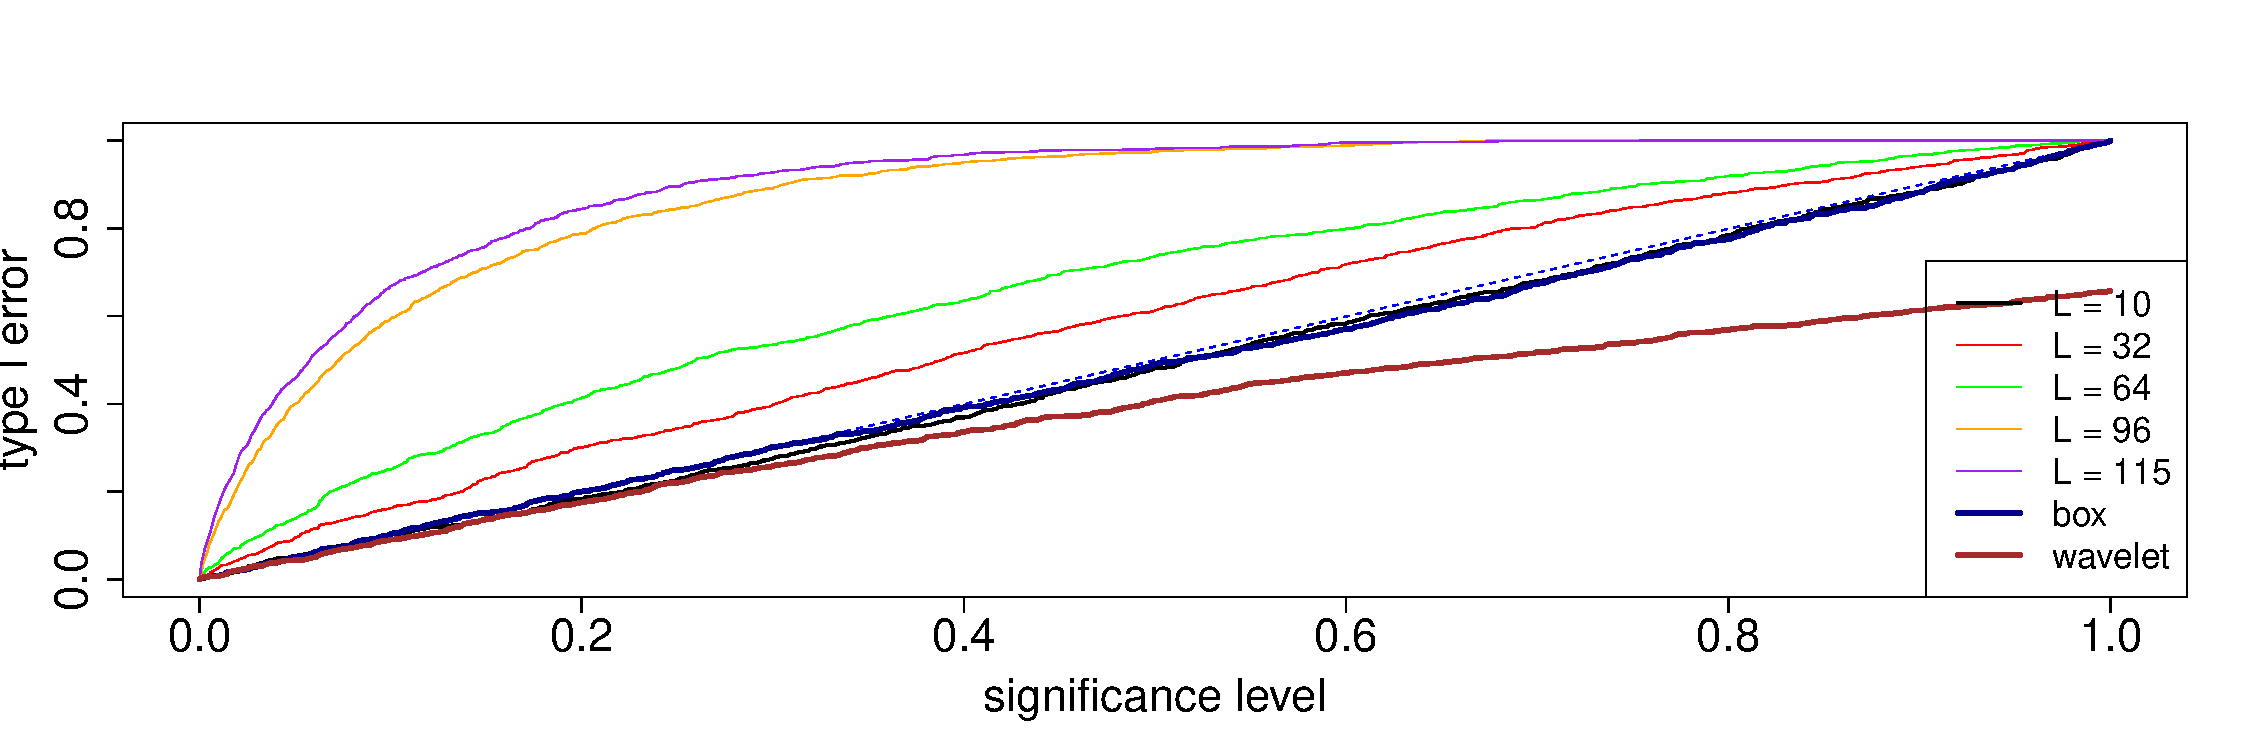
\includegraphics[width=0.7\textwidth]{img/alphaI_testAR.pdf}
	\caption{Сравнение ошибки I рода с другими методами}
	\label{alphaI_testAR}
\end{figure}

\begin{figure}[h!]
	\begin{subfigure}[t]{\textwidth}
		\centering
		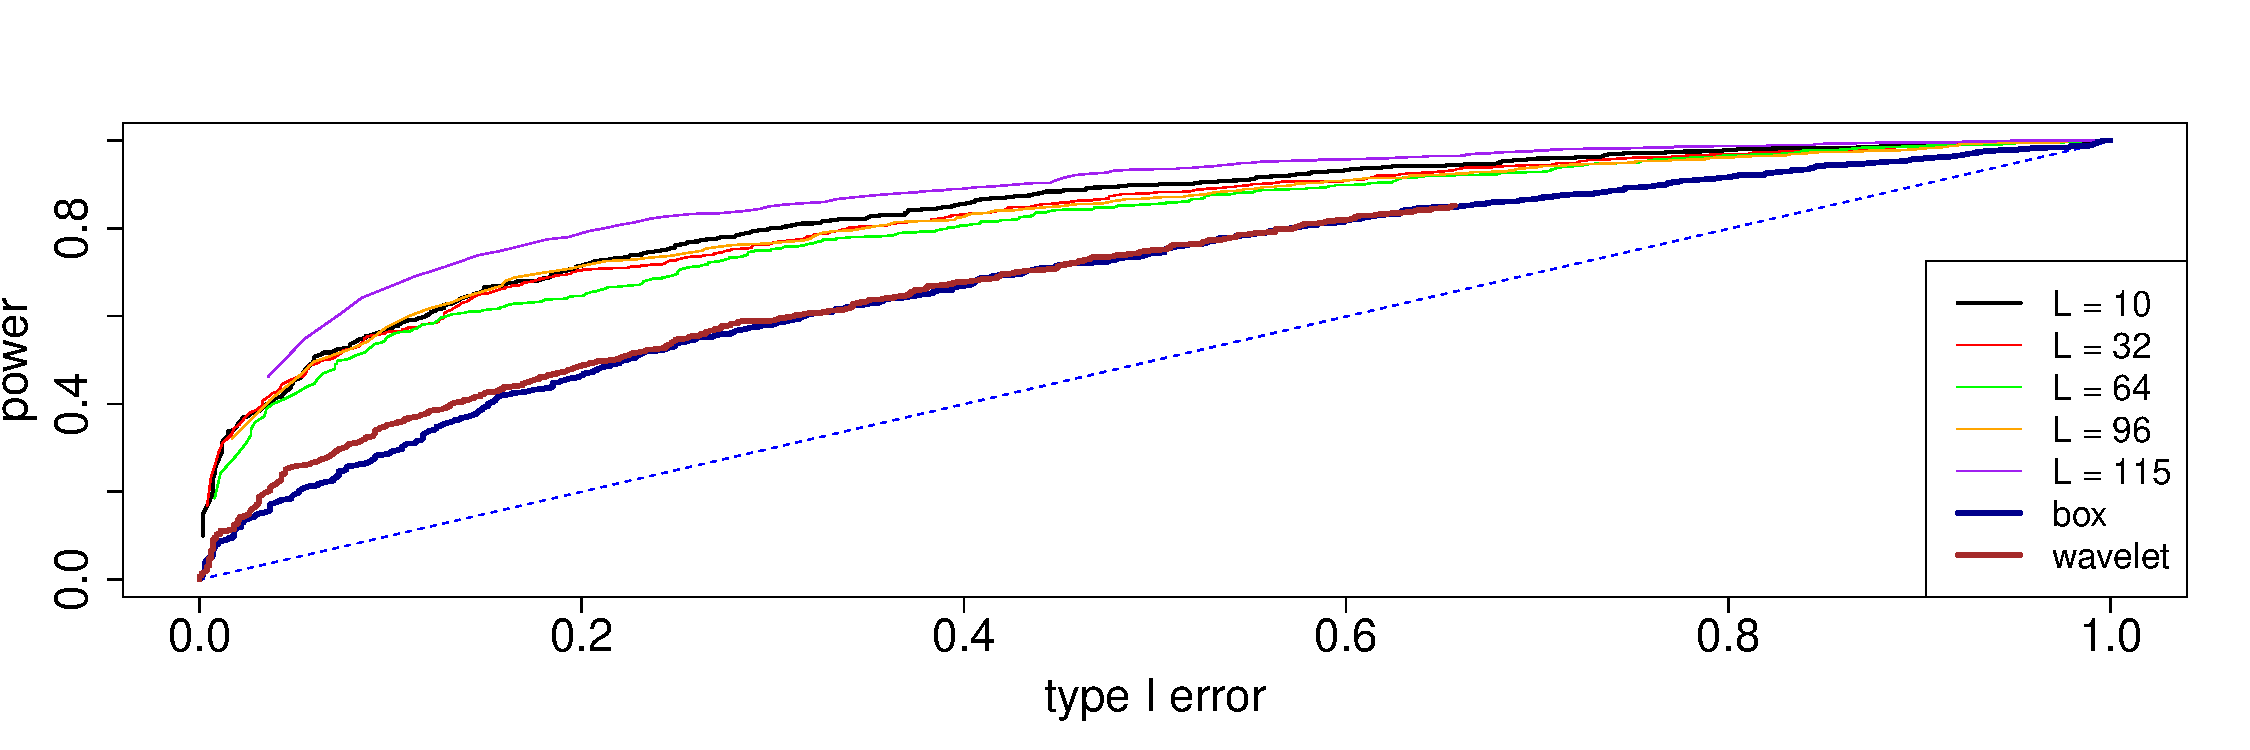
\includegraphics[width=0.7\textwidth]{img/roc_testAR_omega0025.pdf}
		\caption{ROC-кривая ($\omega=0.025$)}
		\label{roc_testAR_omega0025}
	\end{subfigure}
	\begin{subfigure}[t]{\textwidth}
		\centering
		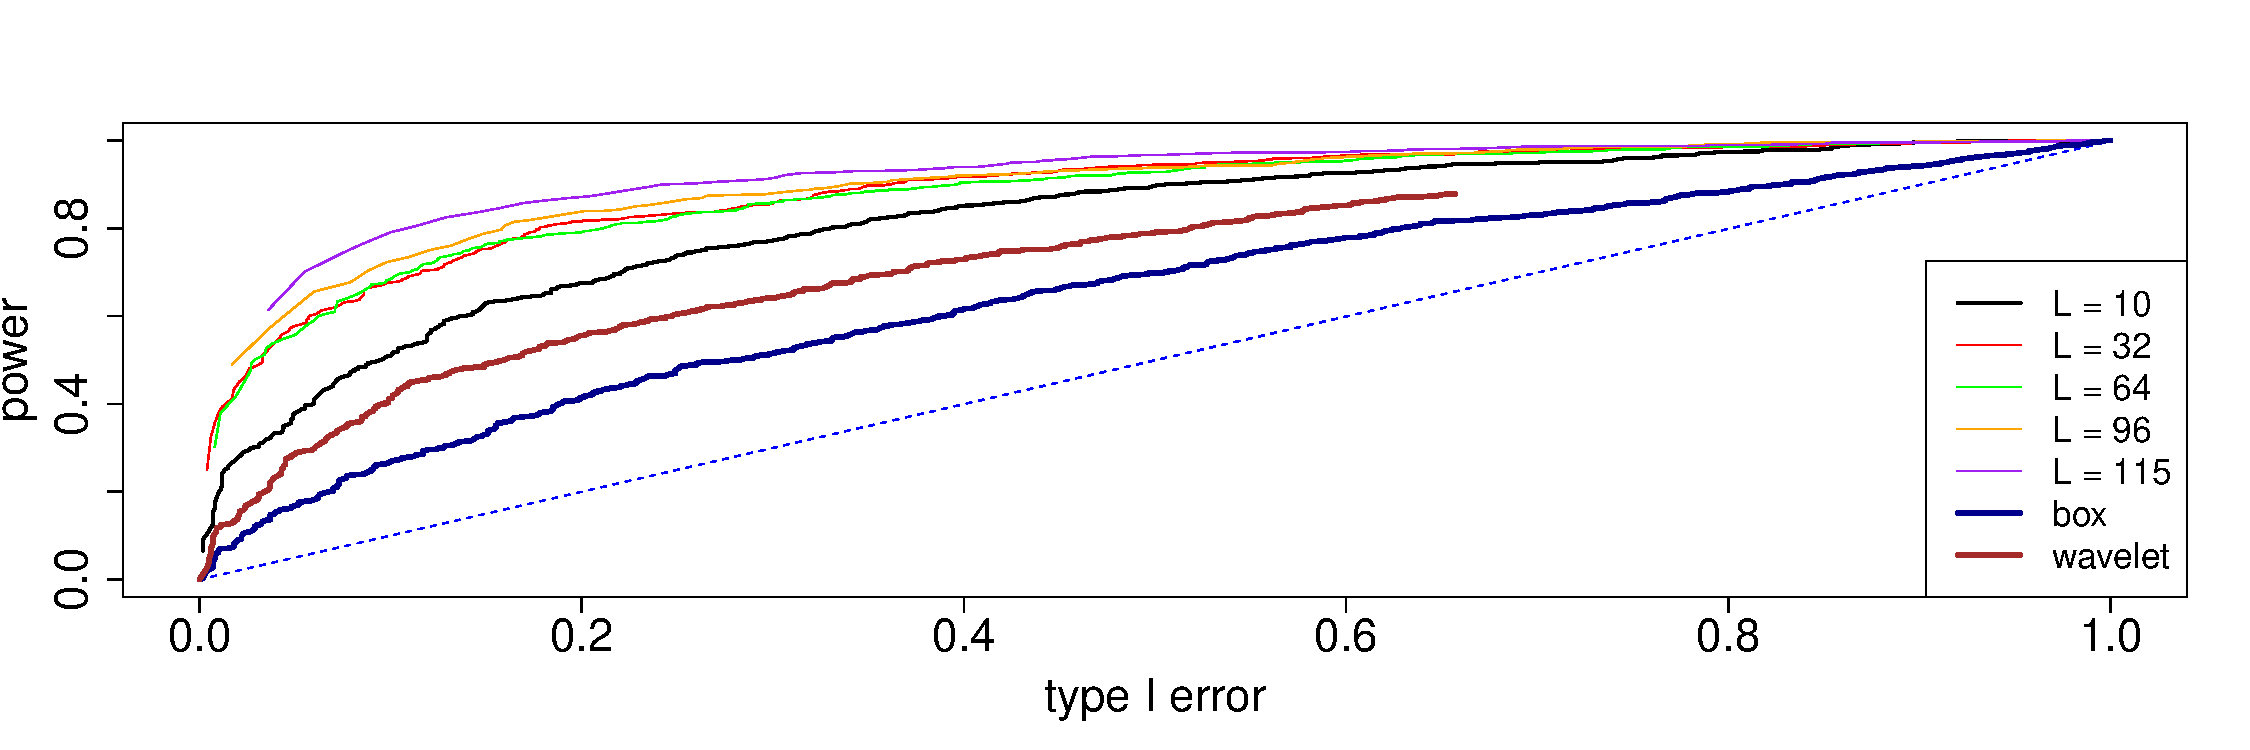
\includegraphics[width=0.7\textwidth]{img/roc_testAR_omega0125.pdf}
		\caption{ROC-кривая ($\omega=0.125$)}
		\label{roc_testAR_omega0125}
	\end{subfigure}
	\begin{subfigure}[t]{\textwidth}
		\centering
		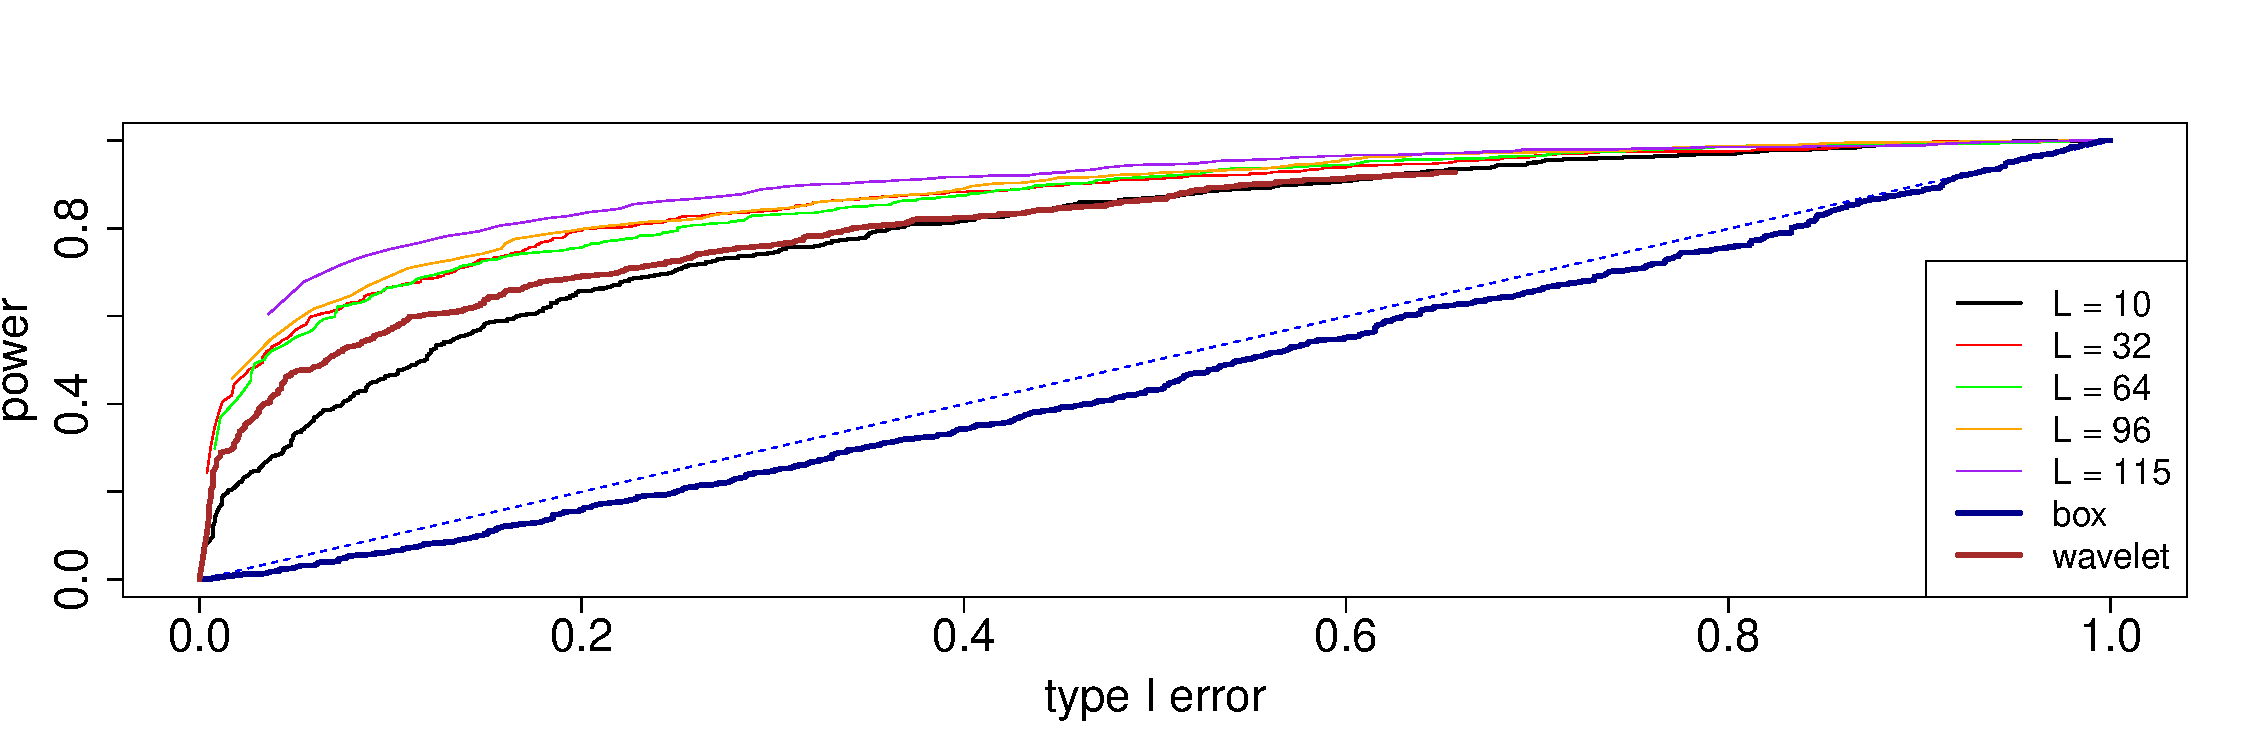
\includegraphics[width=0.7\textwidth]{img/roc_testAR_omega0225.pdf}
		\caption{ROC-кривая ($\omega=0.225$)}
		\label{roc_testAR_omega0225}
	\end{subfigure}
	\caption{Сравнение с другими методами}
\end{figure}

\begin{table}[h!]
	\centering
	\caption{Результаты численного сравнения MC-SSA с другими критериями ($\alpha^*=0.1$)}
	\begin{tabular}{|cc>{\centering\arraybackslash}m{1in}>{\centering\arraybackslash}m{1in} >{\centering\arraybackslash}m{1in}|}\hline
	 Метод & $\alpha_I(\alpha^*)$ & $\beta(\widetilde\alpha^*)$ ($\omega=0.025$) & $\beta(\widetilde\alpha^*)$ ($\omega=0.125$) & $\beta(\widetilde\alpha^*)$ ($\omega=0.225$) \\ 
	  \hline
	MC-SSA ($L=10$) & 0.101 & 0.57 & 0.51 & 0.465 \\ \hline
	  MC-SSA ($L=32$) & 0.163 & 0.566 & 0.678 & 0.668 \\ \hline
	  MC-SSA ($L=64$) & 0.25  & 0.556 & 0.684 & 0.665 \\ \hline
	  MC-SSA ($L=96$) & 0.593 & 0.599 & 0.734 & 0.709 \\ \hline
	  MC-SSA ($L=115$) & 0.668 & 0.668 & 0.791 & 0.753 \\ \hline
	  box & 0.103 & 0.289 & 0.269 & 0.064 \\ \hline
	  wavelet & 0.091 & 0.354 & 0.414 & 0.57 \\ 
	   \hline
	\end{tabular}
	\label{tab:comparison}
\end{table}

На рис.~\ref{roc_testAR_omega0025},~\ref{roc_testAR_omega0125},~\ref{roc_testAR_omega0225} изображены ROC-кривые методов при разных $\omega$. Отметим, что для wavelet построить ROC-кривые для больших ошибок I рода не удалось, поскольку на рис.~\ref{alphaI_testAR} видно, что $\alpha_I(\alpha) < 1$ $\forall \alpha$. Для всех рассмотренных $\omega$ MC-SSA при всех длинах окна мощнее, чем box и wavelet, кроме случая с высокой частотой ($\omega=0.225$), где wavelet оказался немного мощнее MC-SSA с $L=10$. Отметим также, что на рис.~\ref{roc_testAR_omega0225} ROC-кривая метода box лежит ниже прямой $y=x$, поэтому этот тест не имеет смысл применять для выявления высоких частот. Для удобства сравнения в таблице~\ref{tab:comparison} для каждого критерия указана ошибка первого рода и мощность поправленного критерия для каждой рассмотренной альтернативы при уровне значимости $\alpha^*=0.1$.

\section{Monte-Carlo MSSA}\label{sect:mc-mssa}
\subsection{Отличие от одномерного случая}
MC-SSA легко обобщается на многомерный случай: нужно просто заменить SSA на MSSA и генерировать красный шум с тем же количеством каналов, что и у исходного ряда~\cite{mc-mssa}.

Стоит отметить, что, в отличие от одномерного случая, левые и правые векторы матрицы отличаются по построению $\bfX$~\eqref{eq:embedding_mssa}, поэтому в MC-MSSA в качестве векторов для проекции рассмотрены и левые, и правые векторы. Если $W_1,\ldots,W_H$ "--- левые векторы матрицы $\bfX$, метод совпадает с алгоритмом~\ref{alg:multiple_mc-ssa}. Если рассматривать в качестве векторов для проекции правые векторы, то в формулах~\eqref{eq:mc-ssa_statisctics} и~\eqref{eq:mc-ssa_h0} нужно заменить $\bfX$ на $\bfX^\rmT$ и $\mathbf{\Xi}_i$ на $\mathbf{\Xi}_i^\rmT$ соответственно.

\subsection{Численное сравнение модификаций MC-MSSA}\label{mc-mssa_numeric_comparison}
Алгоритм~\ref{alg:correction} поправки радикальных критериев плохо работает для сильно радикальных критериев. Как было показано в~\cite[Приложение  Б.2.4]{Larin_2022}, метод MC-SSA с проекцией на левые (правые) векторы SVD разложения матрицы $\bfX$~\eqref{eq:svd} дает очень радикальный критерий для больших (малых) значений длины окна $L$, что делает невозможным построение поправки.

Однако, в одномерном случае было установлено~\cite{Larin_2022}, что если вместо SVD разложения матрицы $\bfX$ использовать тёплицево, то радикальность критерия уменьшается, и уже можно применить поправку. Установим, что будет в многомерном случае, если использовать модификации, описанные в разделе~\ref{sect:decomposition}.

Пусть количество каналов равно двум, длина каждого канала равна $N=100$, количество суррогатных реализаций красного шума $G=1000$. В качестве альтернативы рассмотрим сигнал $\tS$ с элементами
\[
s_n^{(1)}=s_n^{(2)}=A\cos(2\pi\omega n),\quad n=1,\ldots, N,
\]
Будем смотреть на графики ошибок первого рода и ROC-кривые критериев для длин окна $L=10$, $20$, $50$, $80$, $90$. Будем воспринимать ROC-кривую как график мощности критерия, к которому был применен алгоритм~\ref{alg:correction}.

Введем понятие равномощных критериев. Поскольку оценка мощности критерия $\hat \beta$ является долей отвергнутых нулевых гипотез при верной альтернативе, соответствующий доверительный интервал для настоящего значения $\beta$ выглядит следующим образом:
\[
	\hat \beta \pm z_\alpha \sqrt{\frac{\hat p(1 - \hat p)}M},
\]
где $z_\alpha$ "--- $(1-\alpha/2)$-квантиль $N(0, 1)$ и $M$ "--- количество моделирований. В худшем случае ($\beta=0.5$) доверительный интервал примерно равен $\hat\beta \pm 0.03$. Поэтому будем условно считать критерии равномощными, если их мощности будут отличатся не более чем на $0.03$.

Рассмотрим несколько примеров.

\begin{example}\label{mc-mssa_example1}
	Пусть параметры красного шума $\varphi=0.7$, $\delta=1$ и параметры сигнала $A=1$, $\omega=0.075$.

\begin{figure}[h!]
	\captionsetup[subfigure]{justification=Centering}
	\begin{subfigure}[t]{0.5\textwidth}
		\centering
		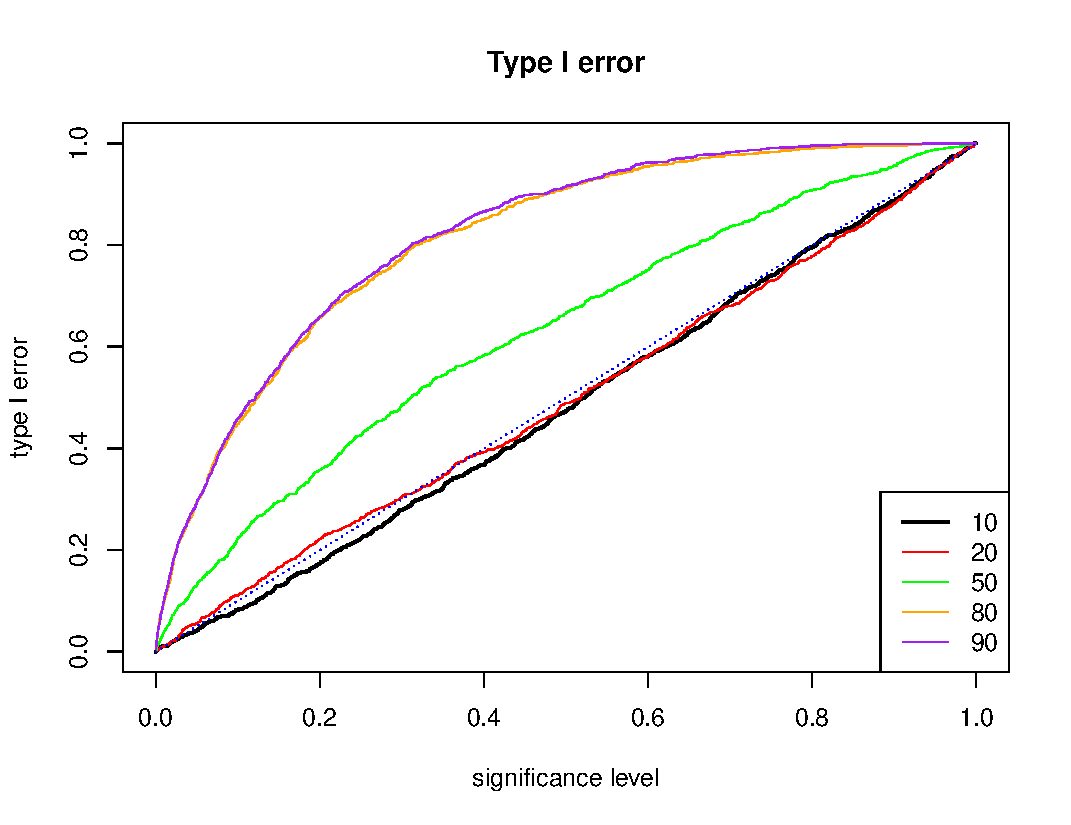
\includegraphics[width=0.9\textwidth]{img/type1error_sum_ev.pdf}
		\caption{Ошибка первого рода (Sum)}
		\label{fig:sum_ev_a}
	\end{subfigure}\hspace{\fill}
	\begin{subfigure}[t]{0.5\textwidth}
		\centering
		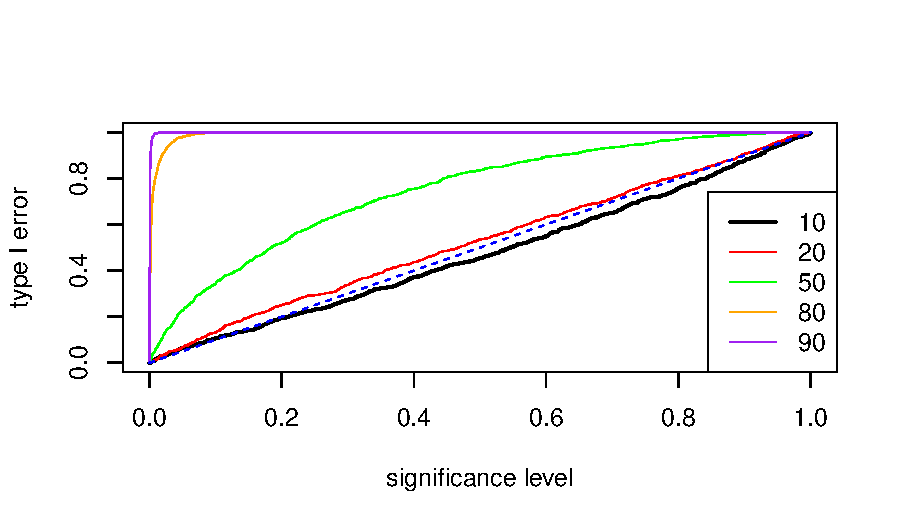
\includegraphics[width=0.9\textwidth]{img/type1error_mssa_ev.pdf}
		\caption{Ошибка первого рода (SVD)}
	\end{subfigure}
	\bigskip
	\begin{subfigure}[t]{0.5\textwidth}
		\centering
		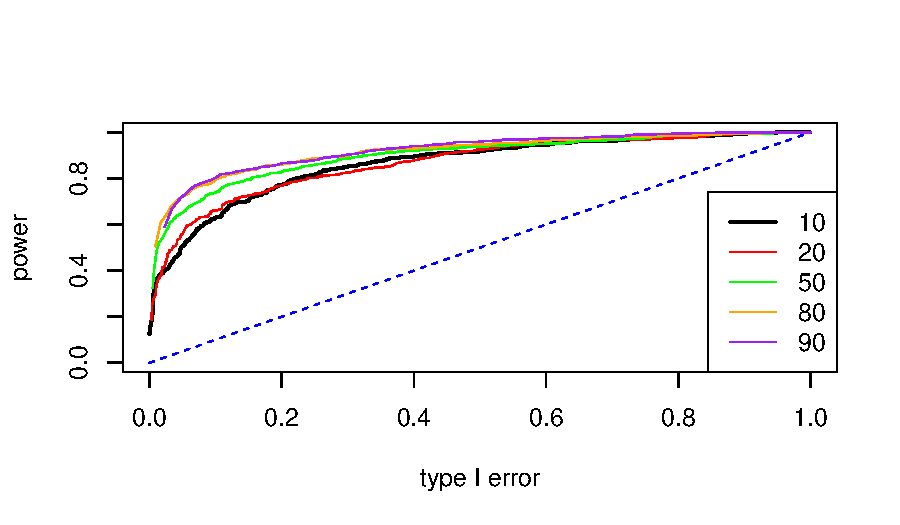
\includegraphics[width=0.9\textwidth]{img/roc_sum_ev_omega0075.pdf}
		\caption{ROC-кривая (Sum)}
		\label{fig:sum_ev_r}
	\end{subfigure}\hspace{\fill}
	\begin{subfigure}[t]{0.5\textwidth}
		\centering
		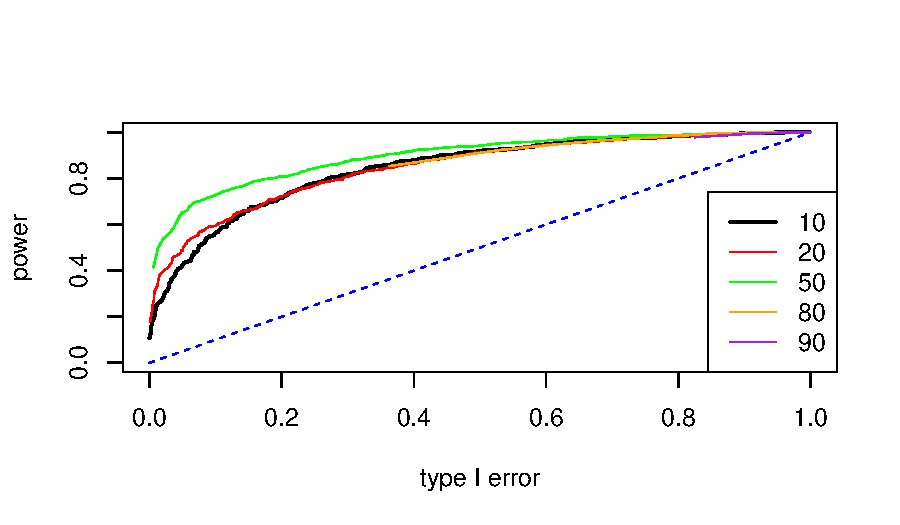
\includegraphics[width=0.9\textwidth]{img/roc_mssa_ev.pdf}
		\caption{ROC-кривая (SVD)}
	\end{subfigure}
	\caption{Сравнение методов с проекцией на левые векторы ($\varphi=0.7$, $\omega=0.075$)}
	\label{fig:sum_ev}
\end{figure}
\begin{figure}[h!]
	\captionsetup[subfigure]{justification=Centering}
	\begin{subfigure}[t]{0.5\textwidth}
		\centering
		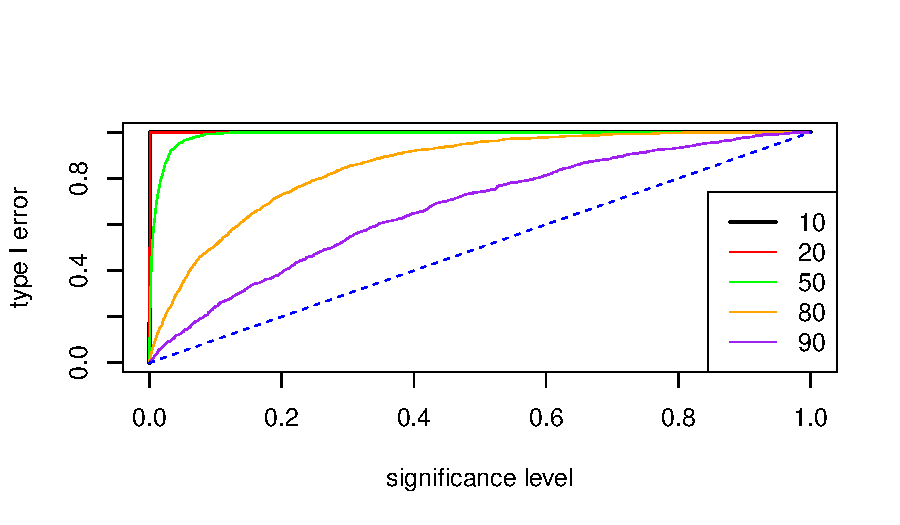
\includegraphics[width=0.9\textwidth]{img/type1error_sum_fa.pdf}
		\caption{Ошибка первого рода (Sum)}
		\label{fig:sum_fa_a}
	\end{subfigure}\hspace{\fill}
	\begin{subfigure}[t]{0.5\textwidth}
		\centering
		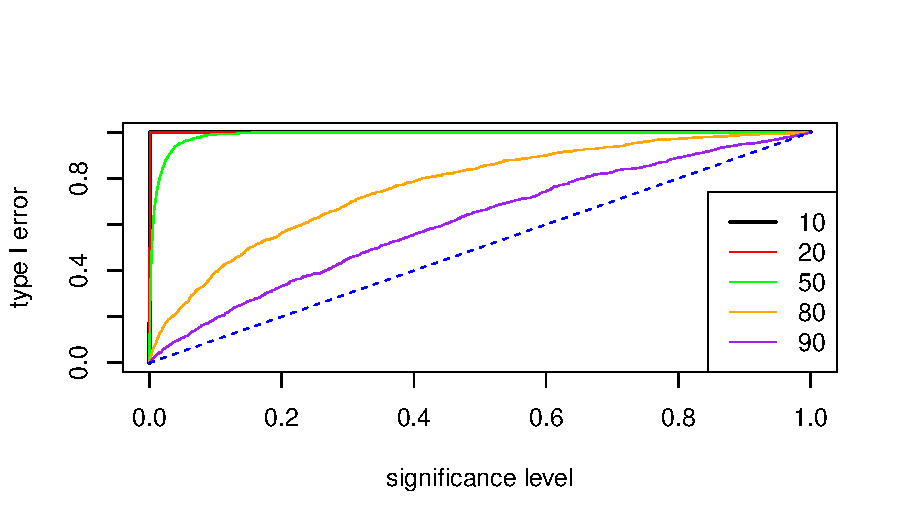
\includegraphics[width=0.9\textwidth]{img/type1error_mssa_fa.pdf}
		\caption{Ошибка первого рода (SVD)}
	\end{subfigure}
	\bigskip
	\begin{subfigure}[t]{0.5\textwidth}
		\centering
		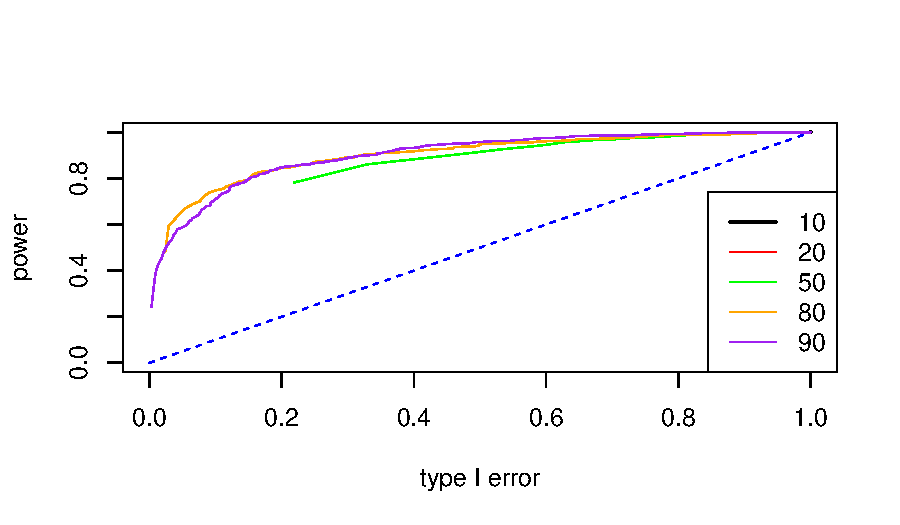
\includegraphics[width=0.9\textwidth]{img/roc_sum_fa_omega0075.pdf}
		\caption{ROC-кривая (Sum)}
		\label{fig:sum_fa_r}
	\end{subfigure}\hspace{\fill}
	\begin{subfigure}[t]{0.5\textwidth}
		\centering
		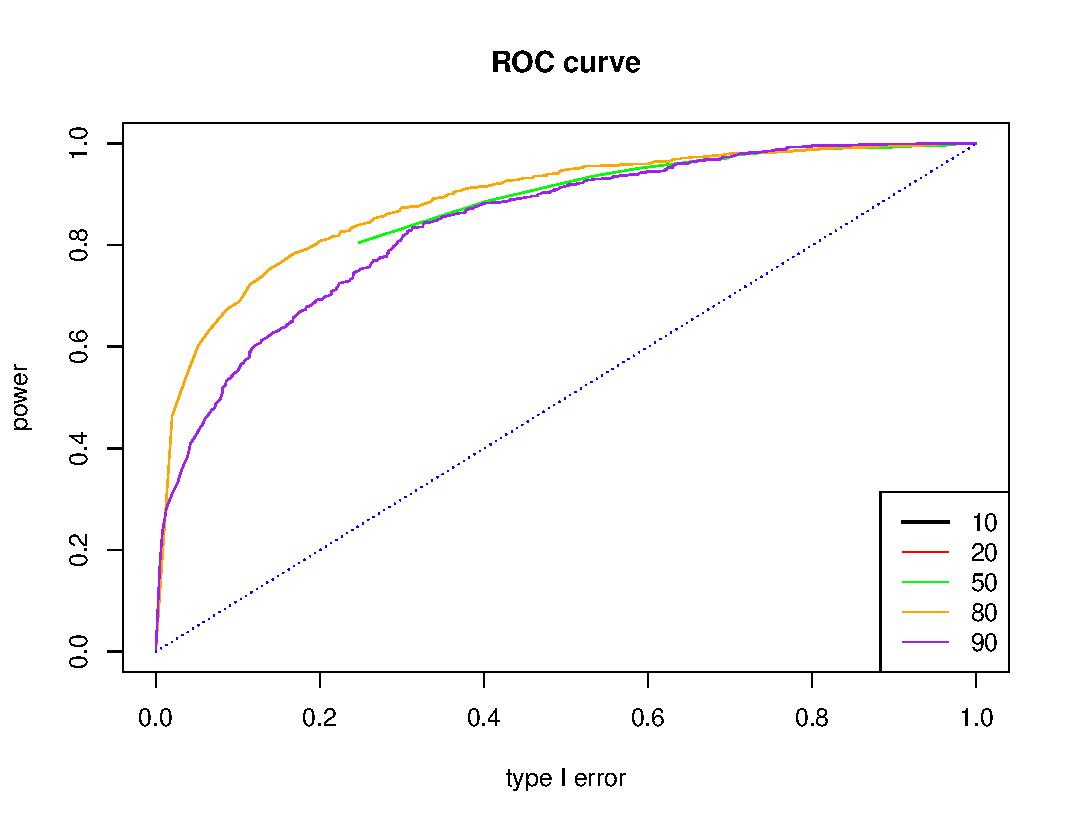
\includegraphics[width=0.9\textwidth]{img/roc_mssa_fa.pdf}
		\caption{ROC-кривая (SVD)}
	\end{subfigure}
	\caption{Сравнение методов с проекцией на правые векторы ($\varphi=0.7$, $\omega=0.075$)}
	\label{fig:sum_fa}
\end{figure}

На рис.~\ref{fig:sum_ev} и~\ref{fig:sum_fa} векторы для проекции были взяты из разложения~\eqref{eq:sum_decomposition}. На рис.~\ref{fig:sum_ev_a} видно, что при $L>20$ метод радикальный, а наибольшая мощность достигается при $L=90$. На рис.~\ref{fig:sum_fa_a} отчетливо заметно, что метод радикальный для всех $L$. Наибольшая мощность наблюдается при $L=80$, но отметим, что из-за слишком большой ошибки первого рода построить ROC-кривую на промежутке $[0,0.22)$ для $L=50$ и на всем промежутке для $L=10$ и $L=20$ не получилось.
\begin{figure}[h!]
	\captionsetup[subfigure]{justification=Centering}
	\begin{subfigure}[t]{0.5\textwidth}
		\centering
		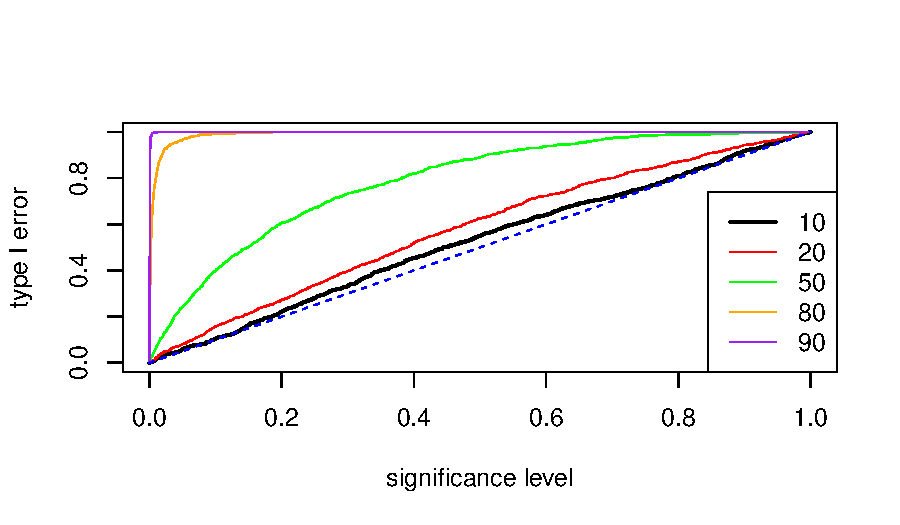
\includegraphics[width=0.9\textwidth]{img/type1error_block_ev.pdf}
		\caption{Ошибка первого рода (Block)}
		\label{fig:block_ev_a}
	\end{subfigure}\hspace{\fill}
	\begin{subfigure}[t]{0.5\textwidth}
		\centering
		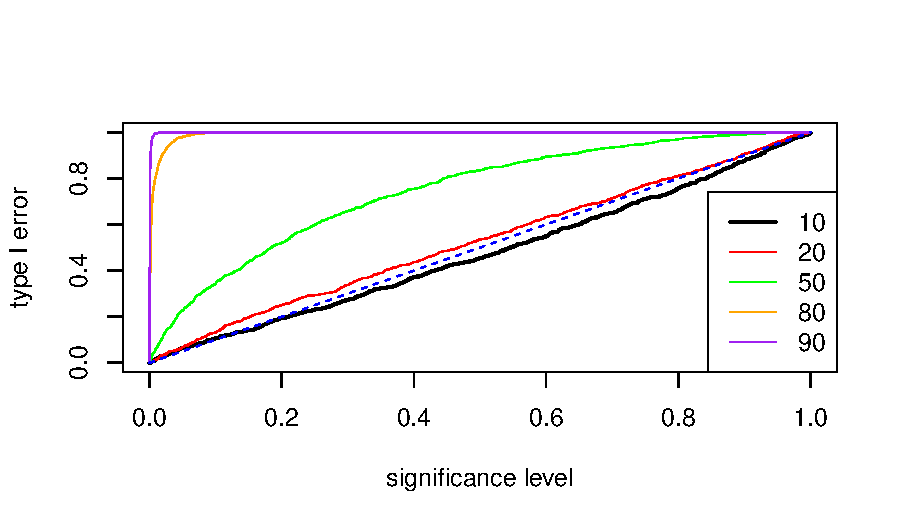
\includegraphics[width=0.9\textwidth]{img/type1error_mssa_ev.pdf}
		\caption{Ошибка первого рода (SVD)}
	\end{subfigure}
	\bigskip
	\begin{subfigure}[t]{0.5\textwidth}
		\centering
		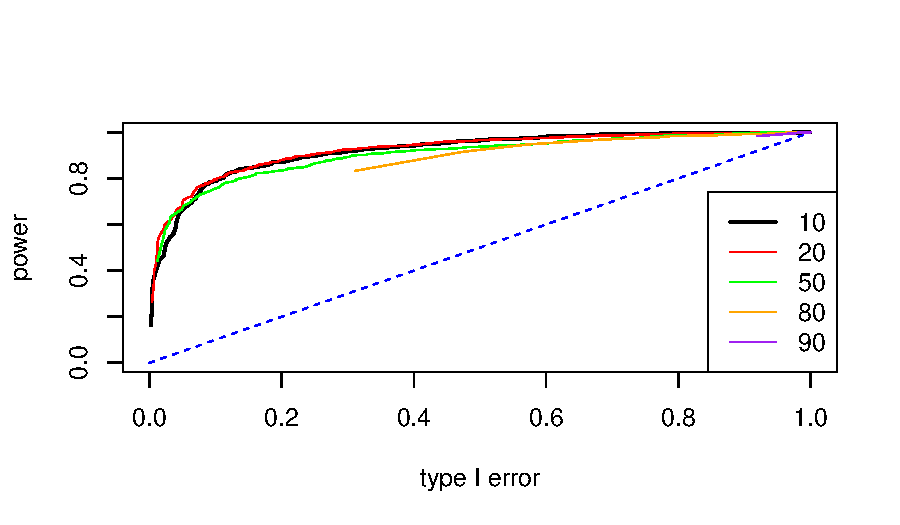
\includegraphics[width=0.9\textwidth]{img/roc_block_ev_omega0075.pdf}
		\caption{ROC-кривая (Block)}
		\label{fig:block_ev_r}
	\end{subfigure}\hspace{\fill}
	\begin{subfigure}[t]{0.5\textwidth}
		\centering
		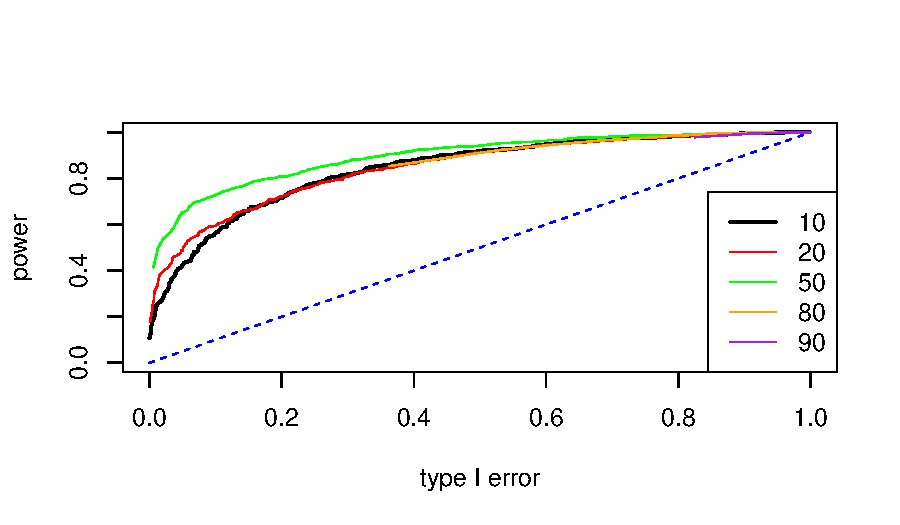
\includegraphics[width=0.9\textwidth]{img/roc_mssa_ev.pdf}
		\caption{ROC-кривая (SVD)}
	\end{subfigure}
	\caption{Сравнение методов с проекцией на левые векторы ($\varphi=0.7$, $\omega=0.075$)}
	\label{fig:block_ev}
\end{figure}
\begin{figure}[h!]
	\captionsetup[subfigure]{justification=Centering}
	\begin{subfigure}[t]{0.5\textwidth}
		\centering
		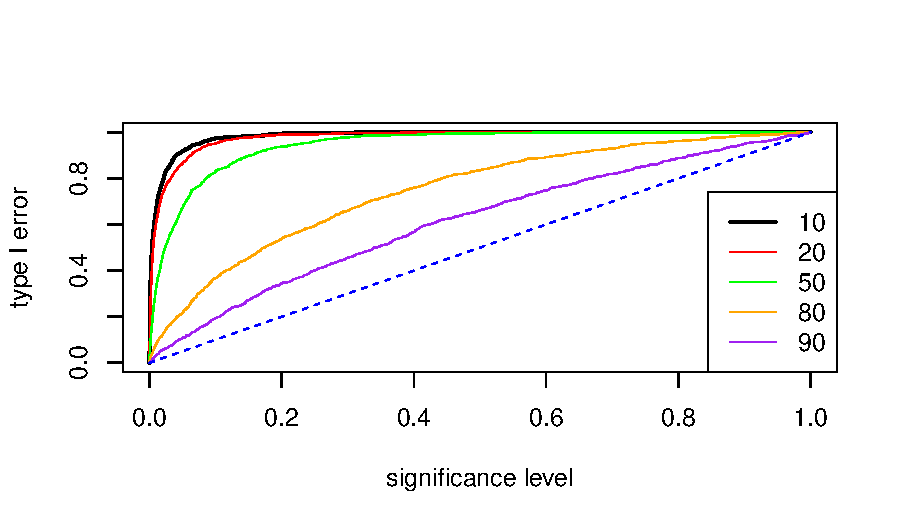
\includegraphics[width=0.9\textwidth]{img/type1error_block_fa.pdf}
		\caption{Ошибка первого рода (Block)}
		\label{fig:block_fa_a}
	\end{subfigure}\hspace{\fill}
	\begin{subfigure}[t]{0.5\textwidth}
		\centering
		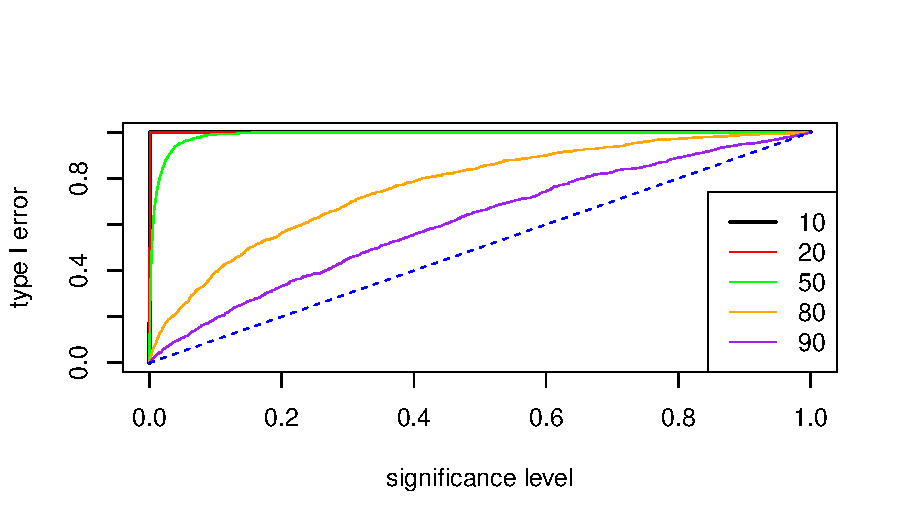
\includegraphics[width=0.9\textwidth]{img/type1error_mssa_fa.pdf}
		\caption{Ошибка первого рода (SVD)}
	\end{subfigure}
	\bigskip
	\begin{subfigure}[t]{0.5\textwidth}
		\centering
		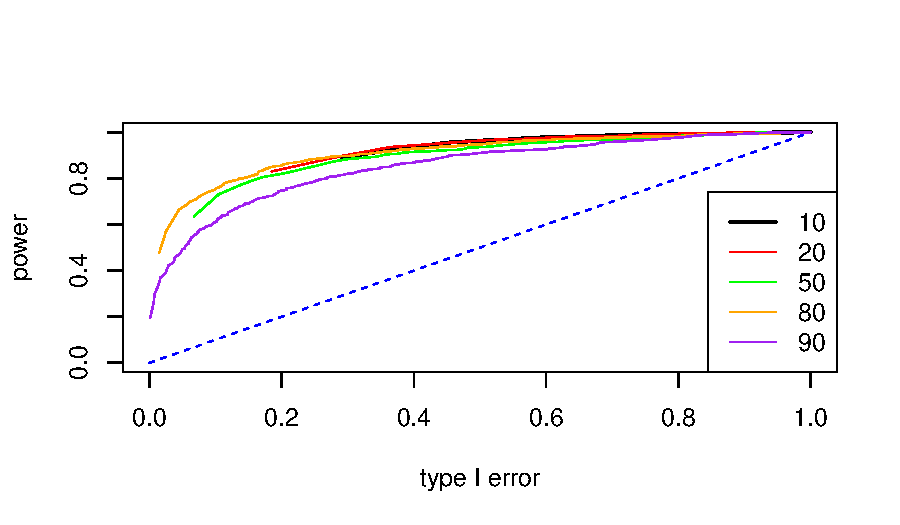
\includegraphics[width=0.9\textwidth]{img/roc_block_fa_omega0075.pdf}
		\caption{ROC-кривая (Block)}
		\label{fig:block_fa_r}
	\end{subfigure}\hspace{\fill}
	\begin{subfigure}[t]{0.5\textwidth}
		\centering
		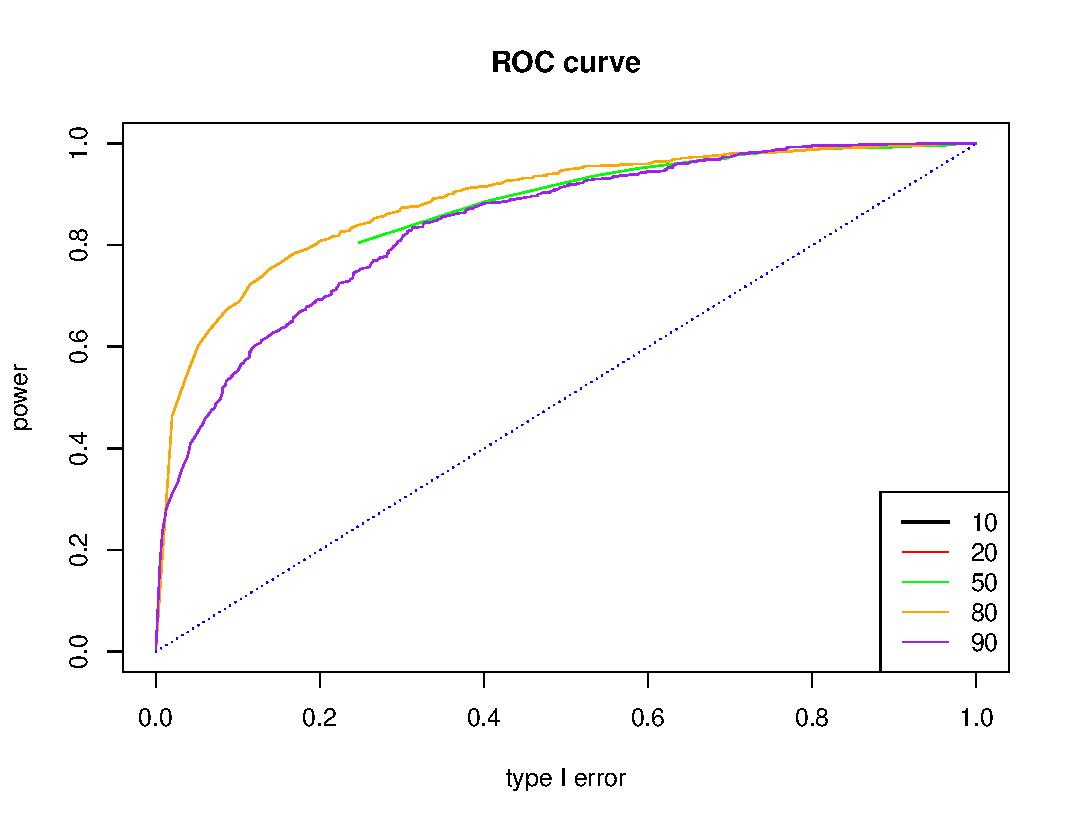
\includegraphics[width=0.9\textwidth]{img/roc_mssa_fa.pdf}
		\caption{ROC-кривая (SVD)}
	\end{subfigure}
	\caption{Сравнение методов с проекцией на правые векторы ($\varphi=0.7$, $\omega=0.075$)}
	\label{fig:block_fa}
\end{figure}

На рис.~\ref{fig:block_ev} и~\ref{fig:block_fa} векторы для проекции были взяты из разложения~\eqref{eq:block_decomposition}. Если рассматривать проекцию на левые векторы, то на рис.~\ref{fig:block_ev_a} видно, что метод радикальный, а наибольшая мощность достигается при $L=20$. Проекция на правые векторы также дает радикальный критерий, как видно на рис.~\ref{fig:block_fa_a}. Наибольшая мощность наблюдается при $L=80$, но из-за слишком большой ошибки первого рода ROC-кривую для $L=10$ и $L=20$, для которых метод, предположительно, имеет б\'oльшую мощность, удалось построить не на всем промежутке.
\begin{table}[h]
	\caption{Численное сравнение методов для оптимальных $L$ ($\varphi=0.7$, $\omega=0.075$)}
	\label{tab:res_mc-ssa}
	\centering
	\begin{tabular}{|c>{\centering\arraybackslash}m{1in}cc>{\centering\arraybackslash}m{1in} >{\centering\arraybackslash}m{1in}cc|}\hline
		Метод & левые/правые векторы & $L$ & $KD$ & длина векторов & количество векторов & $\alpha_I(\alpha^*)$ & $\beta(\widetilde\alpha^*)$ \\
		\hline
		SVD & левые & $50$* &102& $50$ & $50$ & $0.316$ & $0.754$\\
		\hline
		SVD & правые & $80$* &42& $42$ & $42$ & $0.394$ & $0.754$\\
		\hline
		Block & левые & 20, \textcolor{blue}{50}* & 162, 102 & $162$ & $20$ & $0.157$ & $\mathbf{0.796}$ \\
		\hline
		Block & правые & $80$* &42& $80$ & $42$ & $0.367$ & $0.717$\\
		\hline
		Sum & левые & \textcolor{blue}{80}, 90 &42, 22& $90$ & $22$ & $0.535$ & $\mathbf{0.806}$ \\
		\hline
		Sum & правые & $80$* &42& $42$ & $42$ & $0.51$ & $0.748$ \\
		\hline
	\end{tabular}
\end{table}

%В таблице~\ref{tab:res_mc-ssa} для каждого метода указана оптимальная по мощности длина окна (для которой удалось простроить ROC-кривую, звездочкой помечены $L$, которые могут не являться оптимальными), а также ошибка первого рода и мощность поправленного критерия при уровне значимости $\alpha^*=0.1$. Черным выделены максимальная мощность и примерно равные ей. Также для наиболее мощных критериев дополнительно добавлена длина окна, дающая примерно ту же мощность, что и оптимальная, но метод с таким $L$ более эффективный в нахождения левых или правых векторов автоковариационной матрицы (такая длина окна выделена синим). Видно, что MC-MSSA с проекцией на левые или правые векторы обеих модификаций мощнее, чем с проекцией на векторы базового MSSA. Самыми мощными являются методы Block и Sum с проекцией на левые векторы, причем метод Sum более эффективнее (матрица размера $80$ против матрицы размера $162$).
\end{example}

%Далее будем рассматривать только Toeplitz Sum MC-MSSA с проекцией на левые векторы и Toeplitz Block MC-MSSA c проекцией на правые векторы, поскольку именно эти критерии показали уменьшение радикальности по сравнению с базовым MC-MSSA.
\begin{example}~\label{mc-mssa_example2}
	Пусть $\varphi=0.3$, $\delta=1$. Поскольку при уменьшении $\varphi$ уменьшается дисперсия шума и это приводит к увеличению мощности критериев, уменьшим амплитуду сигнала до $A=0.5$.

	\begin{figure}[h!]
		\captionsetup[subfigure]{justification=Centering}
		\begin{subfigure}[t]{0.5\textwidth}
			\centering
			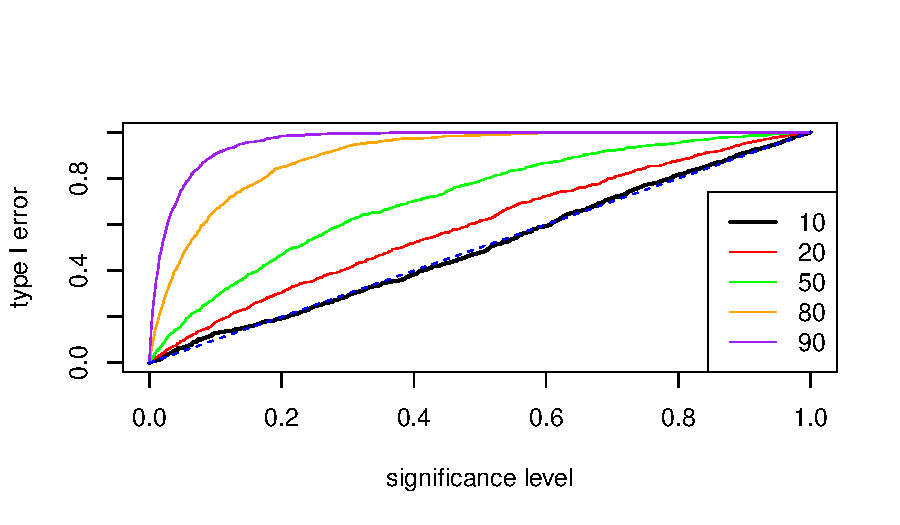
\includegraphics[width=0.95\textwidth]{img/type1error_sum_ev_phi3.pdf}
			\caption{Ошибка I рода (Sum)}
		\end{subfigure}\hspace{\fill}
		\begin{subfigure}[t]{0.5\textwidth}
			\centering
			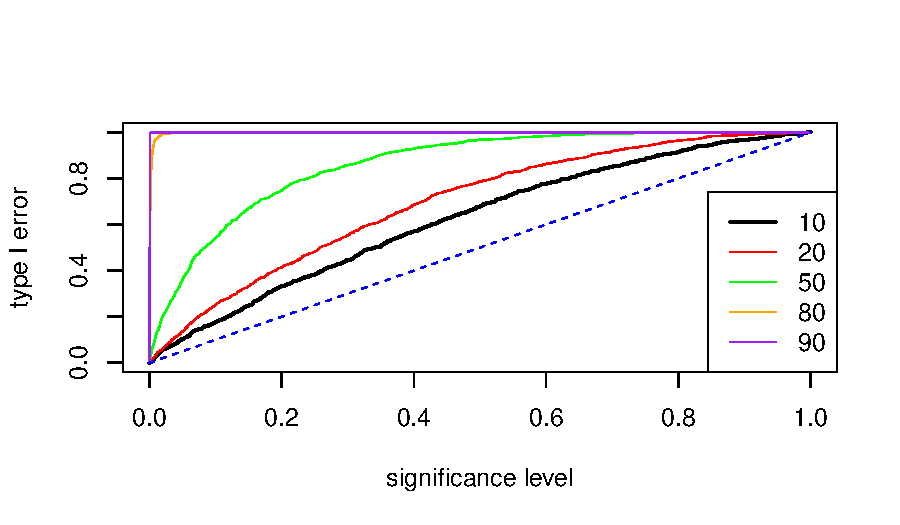
\includegraphics[width=0.95\textwidth]{img/type1error_block_ev_phi3.pdf}
			\caption{Ошибка I рода (Block)}
		\end{subfigure}
		\bigskip
		\begin{subfigure}[t]{0.5\textwidth}
			\centering
			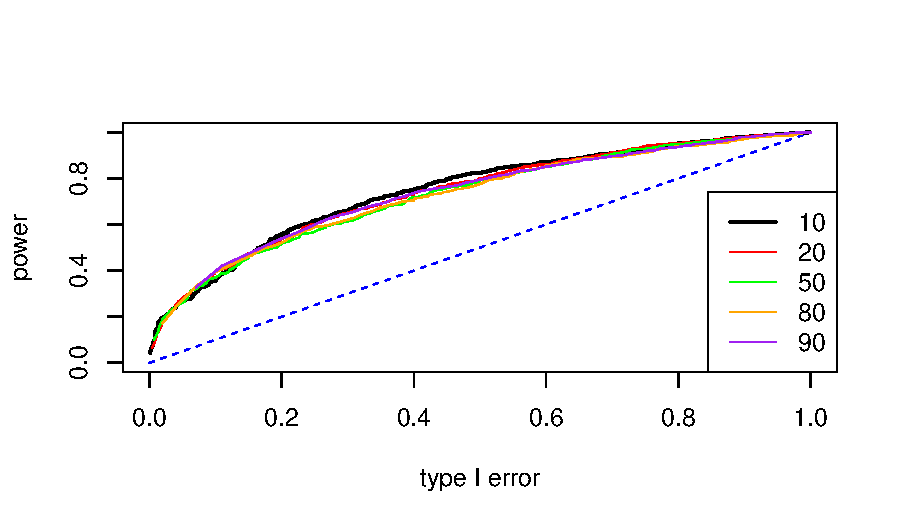
\includegraphics[width=0.95\textwidth]{img/roc_sum_ev_phi3_omega0075.pdf}
			\caption{ROC-кривая (Sum)}
		\end{subfigure}\hspace{\fill}
		\begin{subfigure}[t]{0.5\textwidth}
			\centering
			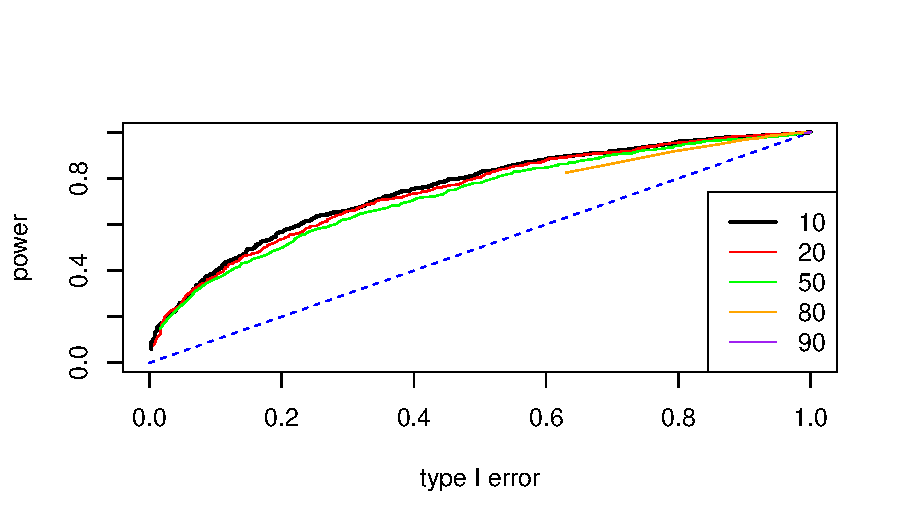
\includegraphics[width=0.95\textwidth]{img/roc_block_ev_phi3_omega0075.pdf}
			\caption{ROC-кривая (Block)}
		\end{subfigure}
		\caption{Сравнение методов с проекцией на левые векторы ($\varphi=0.3$, $\omega=0.075$)}
		\label{fig:sum_block_ev_phi3}
	\end{figure}

	\begin{figure}[h!]
		\captionsetup[subfigure]{justification=Centering}
		\begin{subfigure}[t]{0.5\textwidth}
			\centering
			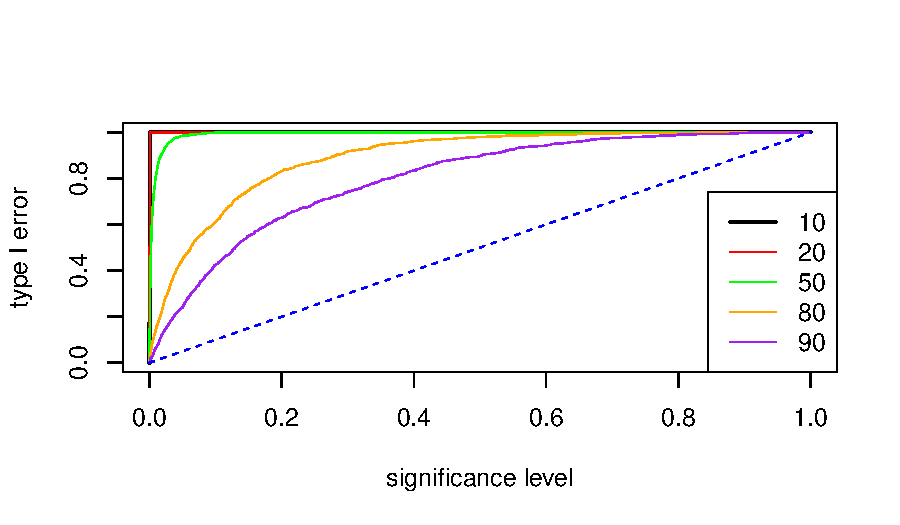
\includegraphics[width=0.95\textwidth]{img/type1error_sum_fa_phi3.pdf}
			\caption{Ошибка I рода (Sum)}
		\end{subfigure}\hspace{\fill}
		\begin{subfigure}[t]{0.5\textwidth}
			\centering
			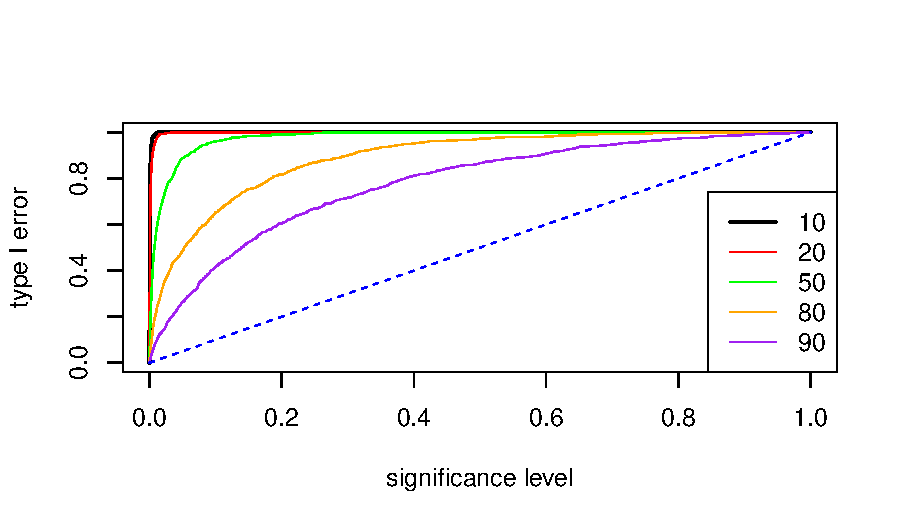
\includegraphics[width=0.95\textwidth]{img/type1error_block_fa_phi3.pdf}
			\caption{Ошибка I рода (Block)}
		\end{subfigure}
		\bigskip
		\begin{subfigure}[t]{0.5\textwidth}
			\centering
			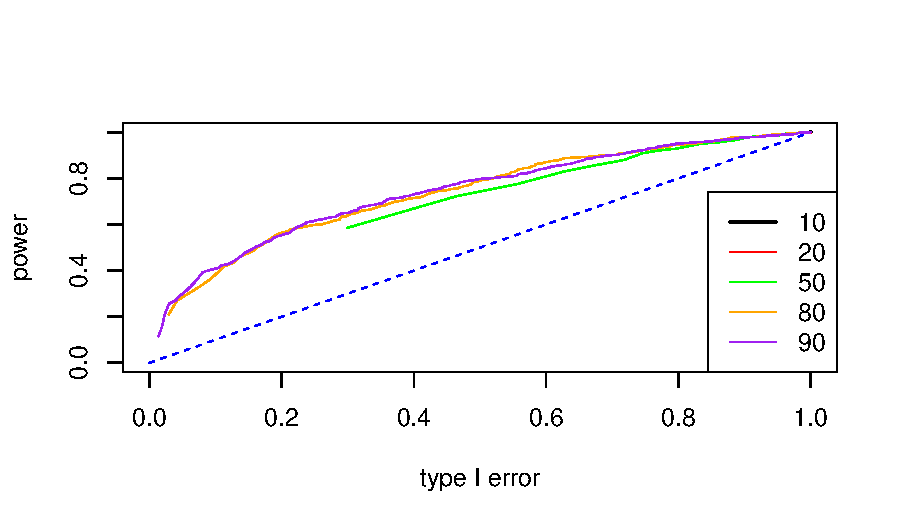
\includegraphics[width=0.95\textwidth]{img/roc_sum_fa_phi3_omega0075.pdf}
			\caption{ROC-кривая (Sum)}
		\end{subfigure}\hspace{\fill}
		\begin{subfigure}[t]{0.5\textwidth}
			\centering
			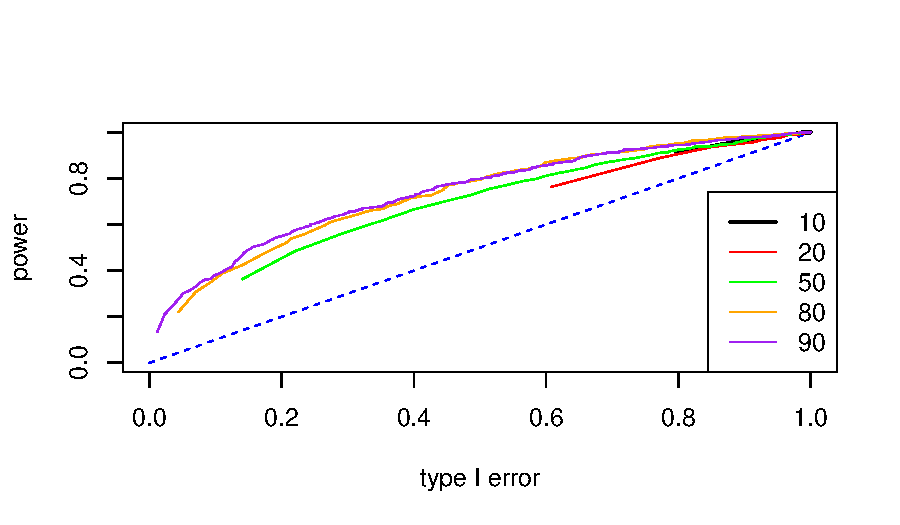
\includegraphics[width=0.95\textwidth]{img/roc_block_fa_phi3_omega0075.pdf}
			\caption{ROC-кривая (Block)}
		\end{subfigure}
		\caption{Сравнение методов с проекцией на правые векторы ($\varphi=0.3$, $\omega=0.075$)}
		\label{fig:sum_block_fa_phi3}
	\end{figure}
	\begin{table}[h]
		\caption{Численное сравнение методов для оптимальных $L$ ($\varphi=0.3$, $\omega=0.075$)}
		\label{tab:res_mc-ssa_phi3}
		\centering
		\begin{tabular}{|c>{\centering\arraybackslash}m{1in}cc>{\centering\arraybackslash}m{1in} >{\centering\arraybackslash}m{1in}cc|}\hline
			Метод & левые/правые векторы & $L$ & $KD$ & длина векторов & количество векторов & $\alpha_I(\alpha^*)$ & $\beta(\widetilde{\alpha}^*)$ \\
			\hline
			SVD & левые & \textcolor{blue}{10}, 20* & 182, 162 & $20$ & $20$ & $0.199$ & $\mathbf{0.399}$ \\
			\hline
			SVD  & правые & \textcolor{blue}{80}, 90* & 42, 22  & $22$ & $22$ & $0.449$ & $0.382$ \\
			\hline
			Block & левые & 10, \textcolor{blue}{20}* & 182, 162 & $182$ & $10$ & $0.177$ & $\mathbf{0.398}$ \\
			\hline
			Block & правые & 80, \textcolor{blue}{90}* & 42, 22 & $90$ & $22$ & $0.414$ & $0.389$\\
			\hline
			Sum & левые & \textcolor{blue}{20}, 90 & 162, 22 & $20$ & $20$ & $0.905$ & $\mathbf{0.421}$ \\
			\hline
			Sum & правые & \textcolor{blue}{80}, 90* & 42, 22 & 22 & $22$ & $0.425$ & $\mathbf{0.412}$ \\
			\hline
		\end{tabular}
	
	\end{table}
	На рис.~\ref{fig:sum_block_ev_phi3} изображены графики ошибок первого рода и ROC-кривые методов Sum и Block с проекцией на левые векторы, а на рис.~\ref{fig:sum_block_fa_phi3} "--- на правые векторы. Как видно по рисункам, при уменьшении параметра $\varphi$, во-первых, увеличивается радикальность критериев для любой длины окна, а во-вторых уменьшается разброс мощности после поправки.
	%В таблице~\ref{tab:res_mc-ssa_phi3} представлены результаты для этого примера. По таблице видно, что различие в мощности у методов совсем небольшое, но все же наибольшая мощность наблюдается у метода Sum с проекцией на левые векторы. Стоит учесть, что из-за слишком сильной радикальности критериев, все приведенные в таблице $L$ могут не являтся оптимальными.
\end{example}

\begin{example}
	В условиях примера~\ref{mc-mssa_example1} увеличим частоту сигнала $\omega$ до $0.225$ и посмотрим на ROC-кривые при такой альтернативе. Поскольку спектральная плотность красного шума монотонно убывает, чем выше частота сигнала, тем он меньше смешивается с красным шумом, следовательно, тем больше мощность критерия. Поэтому уменьшим амплитуду $A$ до $0.4$.

	\begin{figure}
		\captionsetup[subfigure]{justification=Centering}
		\begin{subfigure}[t]{\textwidth}
			\centering
			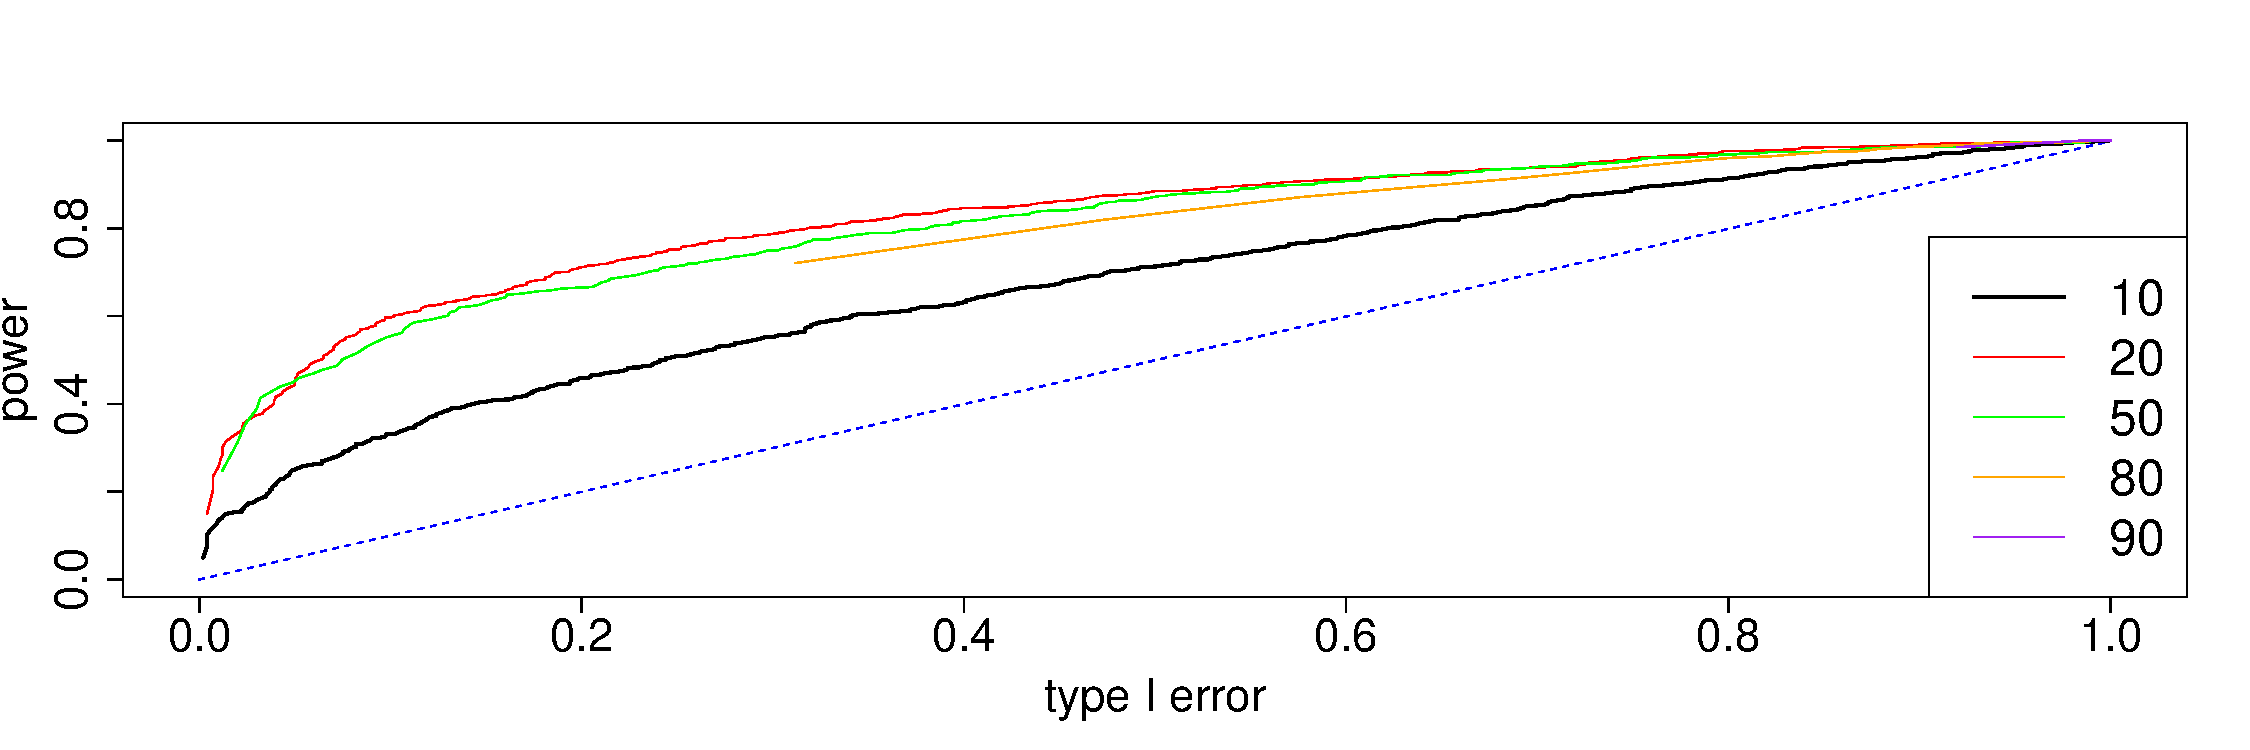
\includegraphics[width=0.7\textwidth]{img/roc_block_ev_omega0225.pdf}
			\caption{Проекция на левые векторы}
		\end{subfigure}\hspace{\fill}
		\begin{subfigure}[t]{\textwidth}
			\centering
			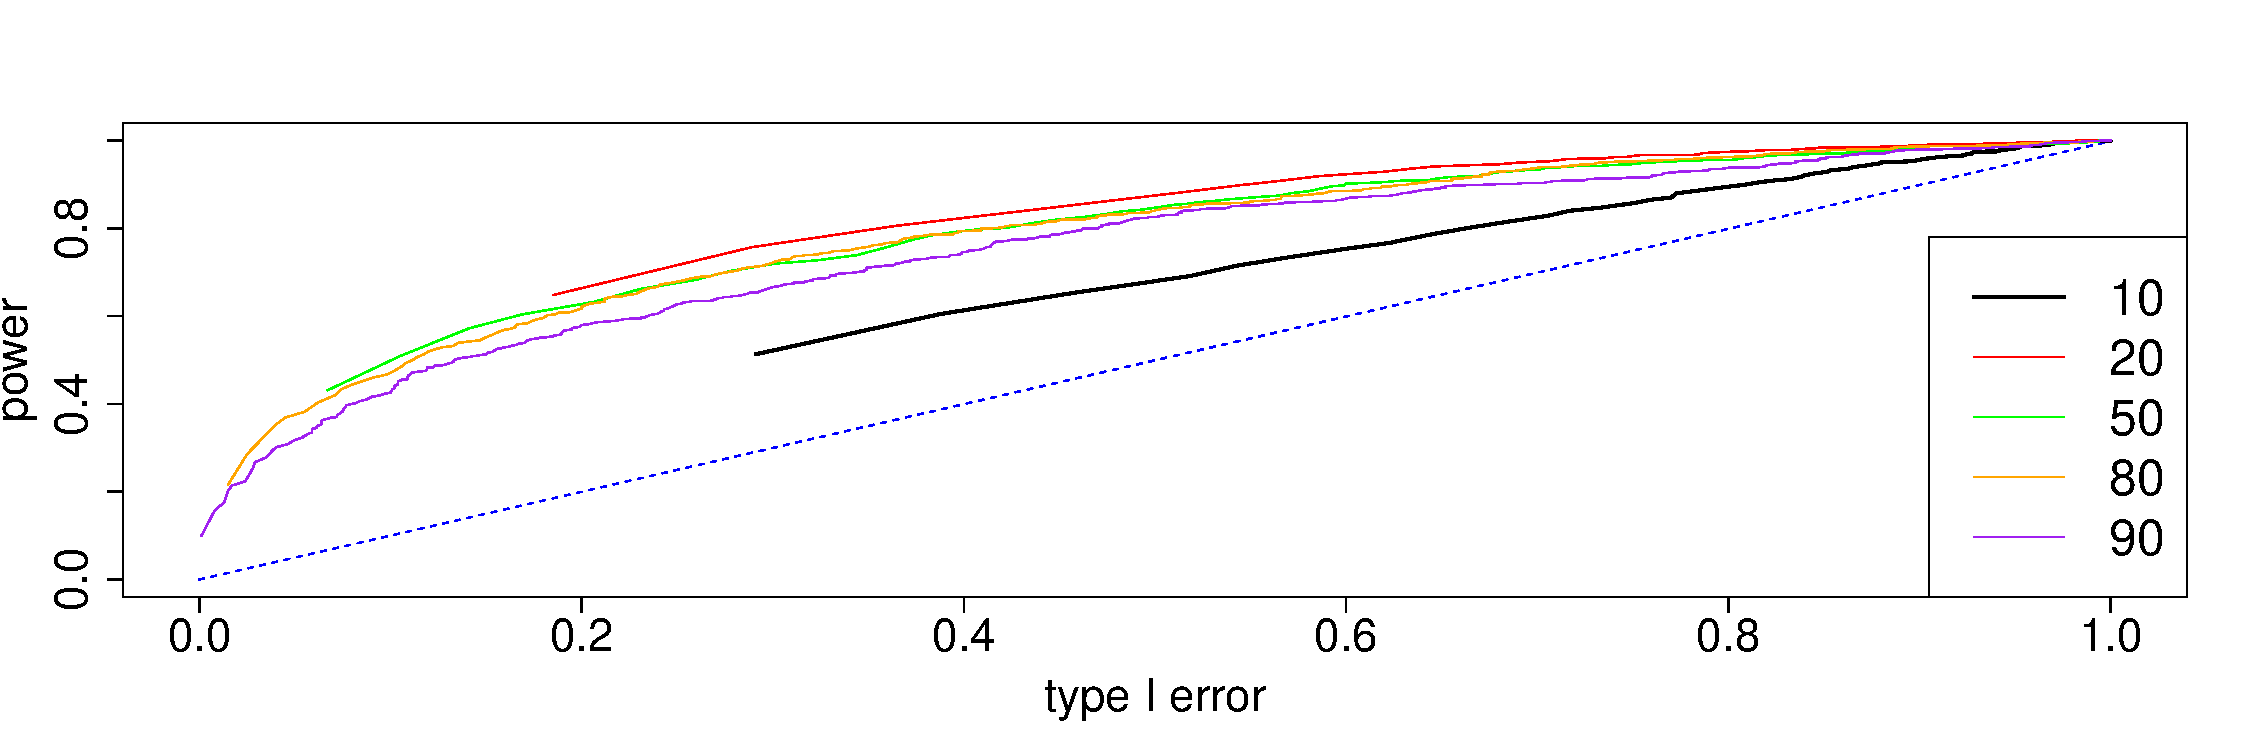
\includegraphics[width=0.7\textwidth]{img/roc_block_fa_omega0225.pdf}
			\caption{Проекция на правые векторы}
		\end{subfigure}
		\caption{ROC-кривые метода Block ($\varphi=0.7$, $\omega=0.225$)}
		\label{fig:block_omega0225}
	\end{figure}
	\begin{figure}[h!]
		\captionsetup[subfigure]{justification=Centering}
		\begin{subfigure}[t]{\textwidth}
			\centering
			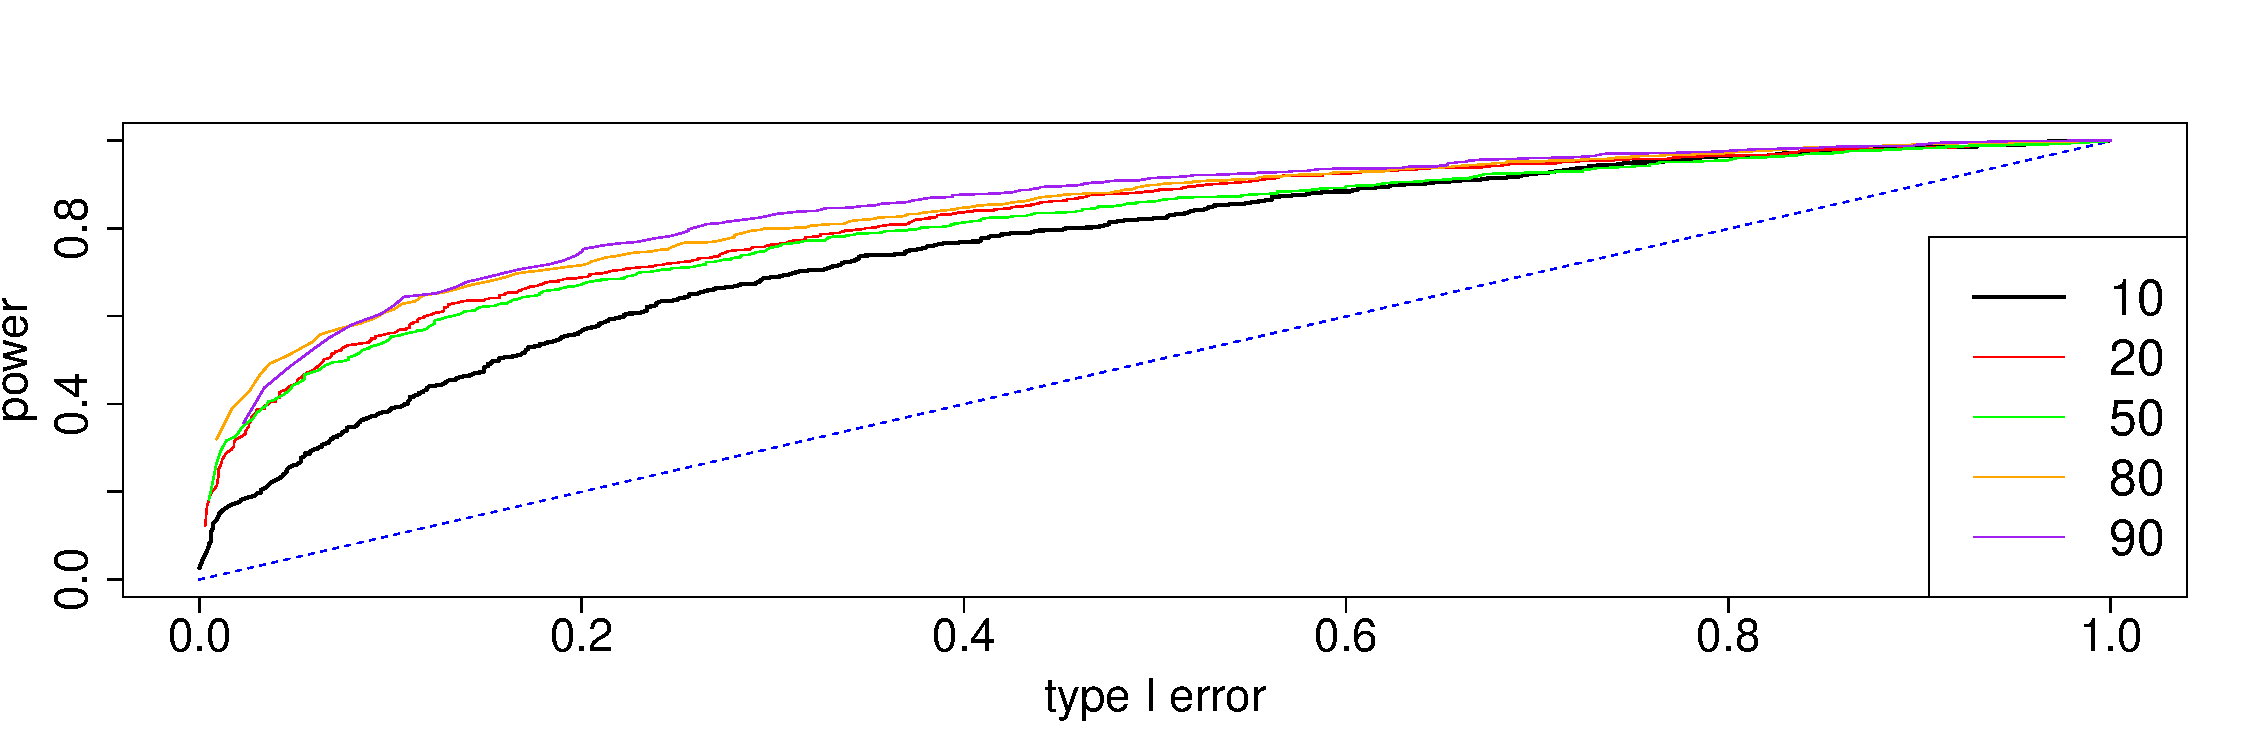
\includegraphics[width=0.7\textwidth]{img/roc_sum_ev_omega0225.pdf}
			\caption{Проекция на левые векторы}
			%\label{fig:block_fa_a}
		\end{subfigure}
		\begin{subfigure}[t]{\textwidth}
			\centering
			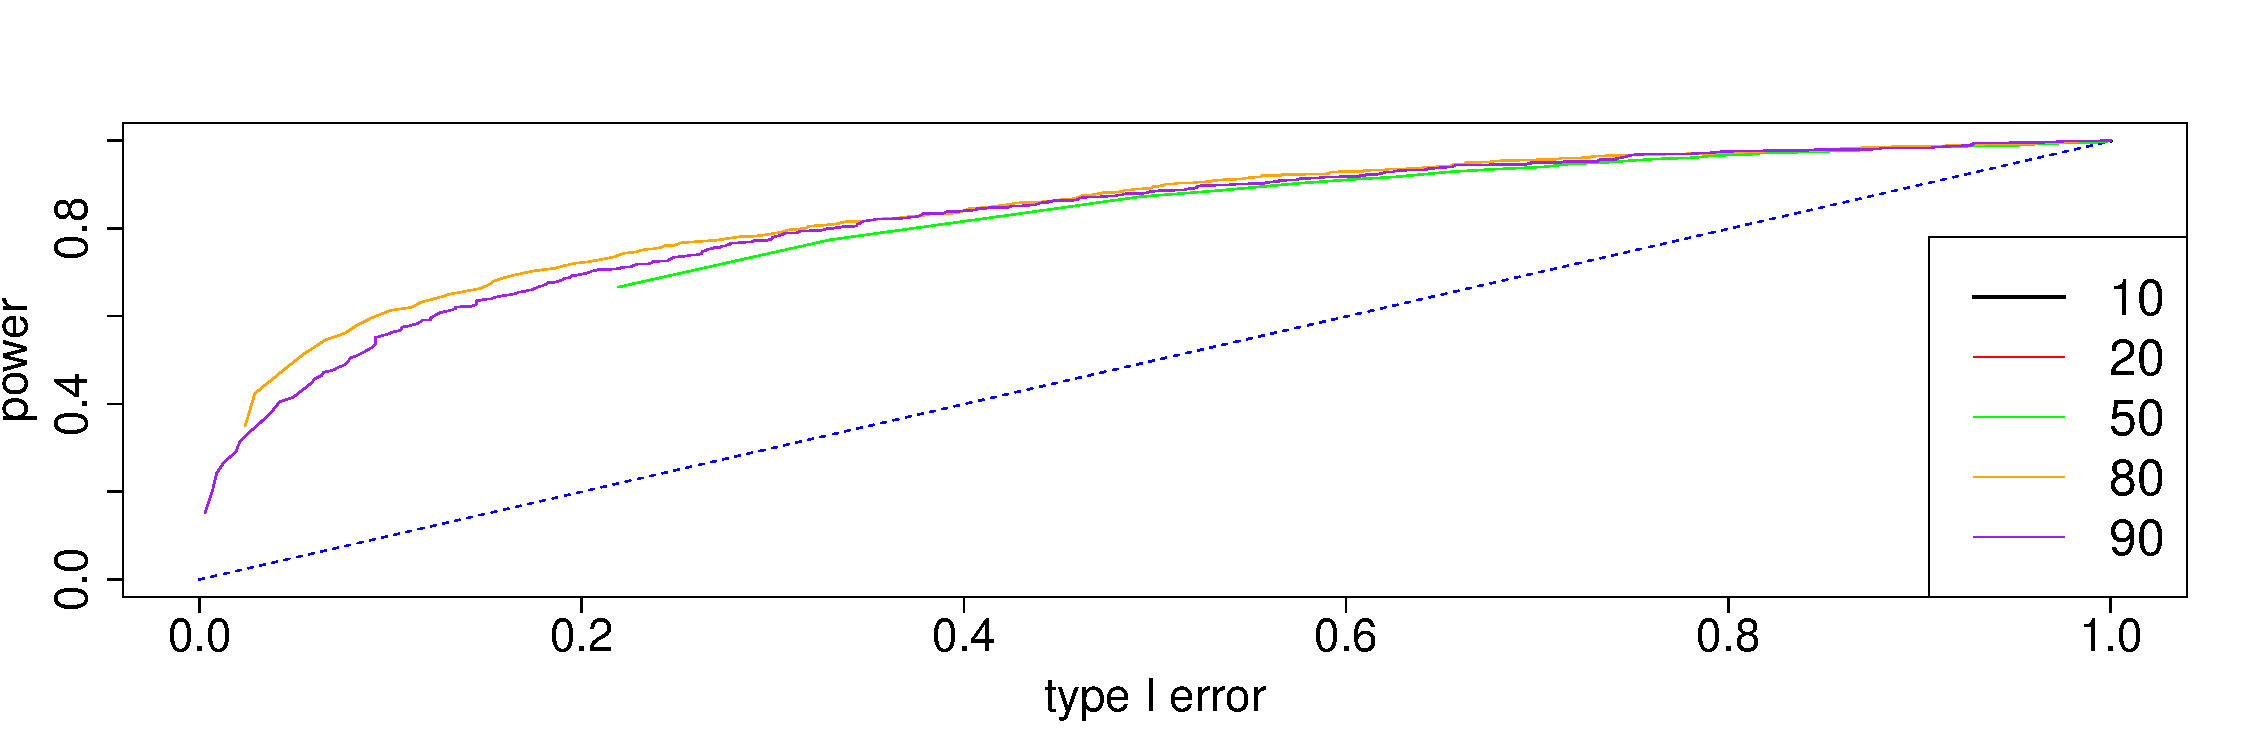
\includegraphics[width=0.7\textwidth]{img/roc_sum_fa_omega0225.pdf}
			\caption{Проекция на правые векторы}
		\end{subfigure}
		\caption{ROC-кривые метода Sum ($\varphi=0.7$, $\omega=0.225$)}
		\label{fig:sum_omega0225}
	\end{figure}
	\begin{table}[h]
		\caption{Численное сравнение методов для оптимальных $L$ ($\varphi=0.7$, $\omega=0.225$)}
		\label{tab:res_mc-mssa_omega0225}
		\centering
		\begin{tabular}{|c>{\centering\arraybackslash}m{1in}cc>{\centering\arraybackslash}m{1in} >{\centering\arraybackslash}m{1in}cc|}\hline
			Метод & левые/правые векторы & $L$ & $KD$ & длина векторов & количество векторов & $\alpha_I(\alpha^*)$ & $\beta(\widetilde{\alpha}^*)$ \\
			\hline
			SVD & левые & $20$* & 162 & $20$ & $20$ & $0.122$ & $0.573$ \\
			\hline
			SVD  & правые & $80$* & 42 & $80$ & $42$ & $0.394$ & $0.442$ \\
			\hline
			Block & левые & $20$* & 162 & $162$ & $20$ & $0.157$ & $\mathbf{0.597}$ \\
			\hline
			Block & правые & 50, \textcolor{blue}{80}* & 102, 42 & $80$ & $42$ & $0.83$ & $0.509$\\
			\hline
			Sum & левые & \textcolor{blue}{80}, 90 & 42, 22 & $10$ & $90$ & $0.535$ & $\mathbf{0.625}$ \\
			\hline
			Sum & правые & $80$* & 42 & $42$ & $42$ & $0.51$ & $\mathbf{0.613}$ \\
			\hline
		\end{tabular}
	
	\end{table}
	На рис.~\ref{fig:sum_omega0225},~\ref{fig:block_omega0225} изображены ROC-кривые критериев. Если сравнить получившиеся графики с графиками на рис~\ref{fig:sum_fa_r},~\ref{fig:sum_fa_r},~\ref{fig:block_ev_r} и~\ref{fig:block_fa_r}, то видно, что с ростом частоты сигнала в альтернативе увеличивается различие в мощности критериев в зависимости от параметра $L$. 
	
	%Также, как и в примере~\ref{mc-mssa_example1}, для наглядного сравнения в таблице~\ref{tab:res_mc-mssa_omega0225} представлены результаты. Метод Sum с проекцией на левые векторы в этом случае дает наибольшую мощность и эффективность.
\end{example}


%Для оценки ошибки первого рода, будем рассматривать красный шум $\bfxi$ с параметрами $\varphi=0.7$ и $\delta=1$, а для оценки мощности будет рассматривать временной ряд $\tX=\tS+\bfxi$, где $\tS$ "--- сигнал с элементами
%\[
%	s_n^{(1)}=s_n^{(2)}=\cos(2\pi\omega n),\quad n=1,\ldots, N,
%\]
%где $\omega=0.075$, $N=100$.

\subsubsection{Выводы}

\begin{table}[h]
	\caption{Мощность методов для оптимальных $L$}
	\label{tab:res_mc-ssa_power}
	\centering
	\begin{tabular}{|c>{\centering\arraybackslash}m{1in}>{\centering\arraybackslash}m{1in}>{\centering\arraybackslash}m{1in}>{\centering\arraybackslash}m{1in}|}\hline
		Метод & левые/правые векторы & $\beta(\widetilde\alpha^*)$ (пример 1) & $\beta(\widetilde\alpha^*)$ (пример 2) & $\beta(\widetilde\alpha^*)$ (пример 3)\\
		\hline
		SVD & левые & 0.754 & \textbf{0.399} & 0.573 \\
		\hline
		SVD & правые & 0.754 & 0.382 & 0.442 \\
		\hline
		Block & левые & \textbf{0.796} & \textbf{0.398} & \textbf{0.597} \\
		\hline
		Block & правые & 0.717 & 0.389 & 0.473 \\
		\hline
		Sum & левые & \textbf{0.806} & \textbf{0.421} & \textbf{0.625} \\
		\hline
		Sum & правые & 0.748 & \textbf{0.412} & \textbf{0.613} \\
		\hline
	\end{tabular}
\end{table}


\begin{table}[h]
	\caption{Трудоемкость методов}
	\label{tab:res_mc-ssa_complexity}
	\centering
	\begin{tabular}{|c>{\centering\arraybackslash}m{1in}>{\centering\arraybackslash}m{1in}>{\centering\arraybackslash}m{1in}>{\centering\arraybackslash}m{1in}|}\hline
		Метод & левые/правые векторы & Размер матрицы (пример 1) & Размер матрицы (пример 2) & Размер матрицы (пример 3) \\
		\hline
		SVD & левые & 50 & 10 & 20 \\
		\hline
		SVD & правые & 80 & 80 & 80 \\
		\hline
		Block & левые & 102 & 162 & 162 \\
		\hline
		Block & правые & 42 & 22 & 42\\
		\hline
		Sum & левые & 80 & 20 & 80 \\
		\hline
		Sum & правые & 80 & 80 & 80 \\
		\hline
	\end{tabular}
\end{table}

Подведем итоги. В таблице~\ref{tab:res_mc-ssa_power} представлены мощность поправленных критериев при уровне значимости $\alpha^*=0.1$ для оптимальной длины окна для всех рассмотренных примеров, а в таблице~\ref{tab:res_mc-ssa_complexity} представлены размеры матриц методов, у которых находятся вектора для проекции для тех длин окна, мощность которых примерно равна мощности при оптимальном $L$, но критерии с такой длиной окна более эффективные (матрица меньшего размера). Для рассмотренных примеров методы Block Sum c проекцией на левые векторы показывают наибольшую мощность среди всех рассмотренных модификаций MC-MSSA, однако метод Sum во всех трех случаях численно эффективнее метода Block в нахождении векторов для проекции. Также хочется отметить, что метод Sum с проекцией на левые векторы дает наименее радикальный критерий, что важно при построении поправки (см. замечание~\ref{remark:large_G}). Также отметим, что из-за слишком сильной радикальности остальных критериев определить длину окна, дающую наибольшую мощность, затруднительно, поэтому нужно отдельно исследовать проблему выбора оптимального $L$. Но на данный момент, беря в учет рассмотренные примеры и результаты раздела~\ref{sect:mssa_comparison}, рекомендуется использовать метод Sum с проекцией на левые векторы c $L=90$ для рядов длины $N=100$.

%Также все методы, кроме Sum, с проекцией на левые вектора сильно радикальные. Поэтому рекомендуется использовать вариант Sum с проекцией на левые векторы с $L=90$. 

\chapter{Метод Monte-Carlo SSA для реальных задач}\label{chpt:mc_ssa_real}
В главе~\ref{chpt:mc-ssa} предполагалось, что параметры шума известны и нет мешающего сигнала (например, сезонности или тренда). Мешающий сигнал "--- это сигнал, который уже не нужно обнаруживать при проверки гипотезы о наличии сигнала.  В этой главе рассмотрим случаи, которые более близки к реальным задачам.

В разделе~\ref{sect:cps2024} исследована зависимость радикальности и мощности MC-SSA от длины окна на различных примерах. В разделе~\ref{sect:phi_est} рассмотрены два способа оценки параметров красного шума и их численное сравнение в точности оценивания и мощности MC-SSA. В разделе~\ref{sect:nuisance} приведены два алгоритма модификации MC-SSA с мешающим сигналом и проведено численное исследование методов для разных примеров мешающего сигнала. В разделе~\ref{sect:examples} рассмотрены примеры реальных временных рядов и их анализ с помощью SSA и MC-SSA.

%В этой главе рассмотрены способы оценки параметров красного шума, описан метод MC-SSA с мешающим сигналом, исследована зависимость радикальности и мощности MC-SSA от длины окна $L$, а также рассмотрены несколько реальных временных рядов.

\section{Зависимость радикальности и мощности от параметра $L$}~\label{sect:cps2024}
Поскольку рассматриваемый вариант критерия MC-SSA является радикальным, существует проблема выбора такой длины окна $L$, которая дает максимально мощный критерий, но при этом не слишком радикальный, чтобы можно было применить поправку. Однако, в зависимости от длины ряда $N$ и параметров красного шума $\bfxi$ наблюдаются разные зависимости мощности от $L$.

Рассмотрим несколько примеров. Пусть дана модель
\[
    \tX=\tS+{\boldsymbol\xi},
\]
где $\tS=\{A\cos(2\pi\omega n)\}_{n=1}^N$, а ${\boldsymbol\xi}$ "--- красный шум с параметрами $\varphi$ и $\delta=1$. Рассмотрим следующие нулевую гипотезу и альтернативу: $H_0:A=0$, $H_1:A\ne0$. В этом разделе будем предполагать, что параметры красного шума известны. В первых трех примерах рассмотрим частоту сигнала $\omega = 0.075$.

\begin{example}\label{example1}
	Пусть $\varphi=0.7$, $N=100$.
	\begin{figure}[h!]
		\captionsetup[subfigure]{justification=Centering}
		\begin{subfigure}[t]{\textwidth}
			\centering
			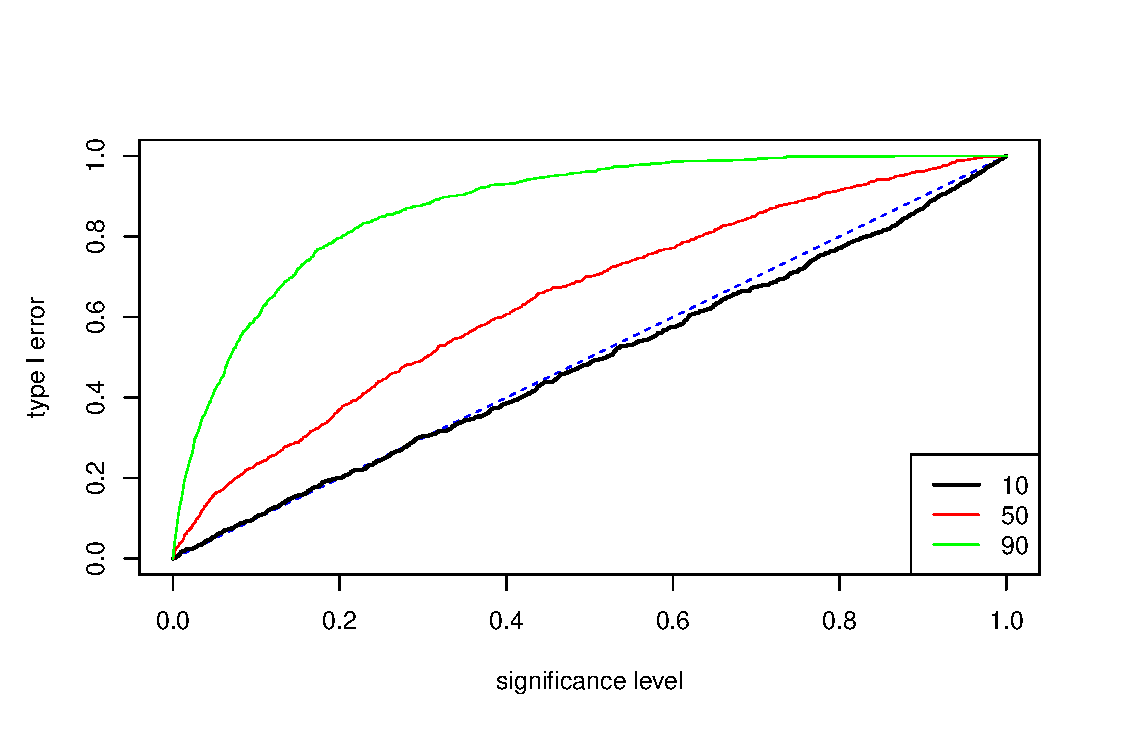
\includegraphics[width=0.7\textwidth]{../cps2024/images/alphaI_phi7_N100.eps}
			\caption{Ошибка I рода}
			\label{alphaI_phi7_N100}
		\end{subfigure}
		\begin{subfigure}[t]{\textwidth}
			\centering
			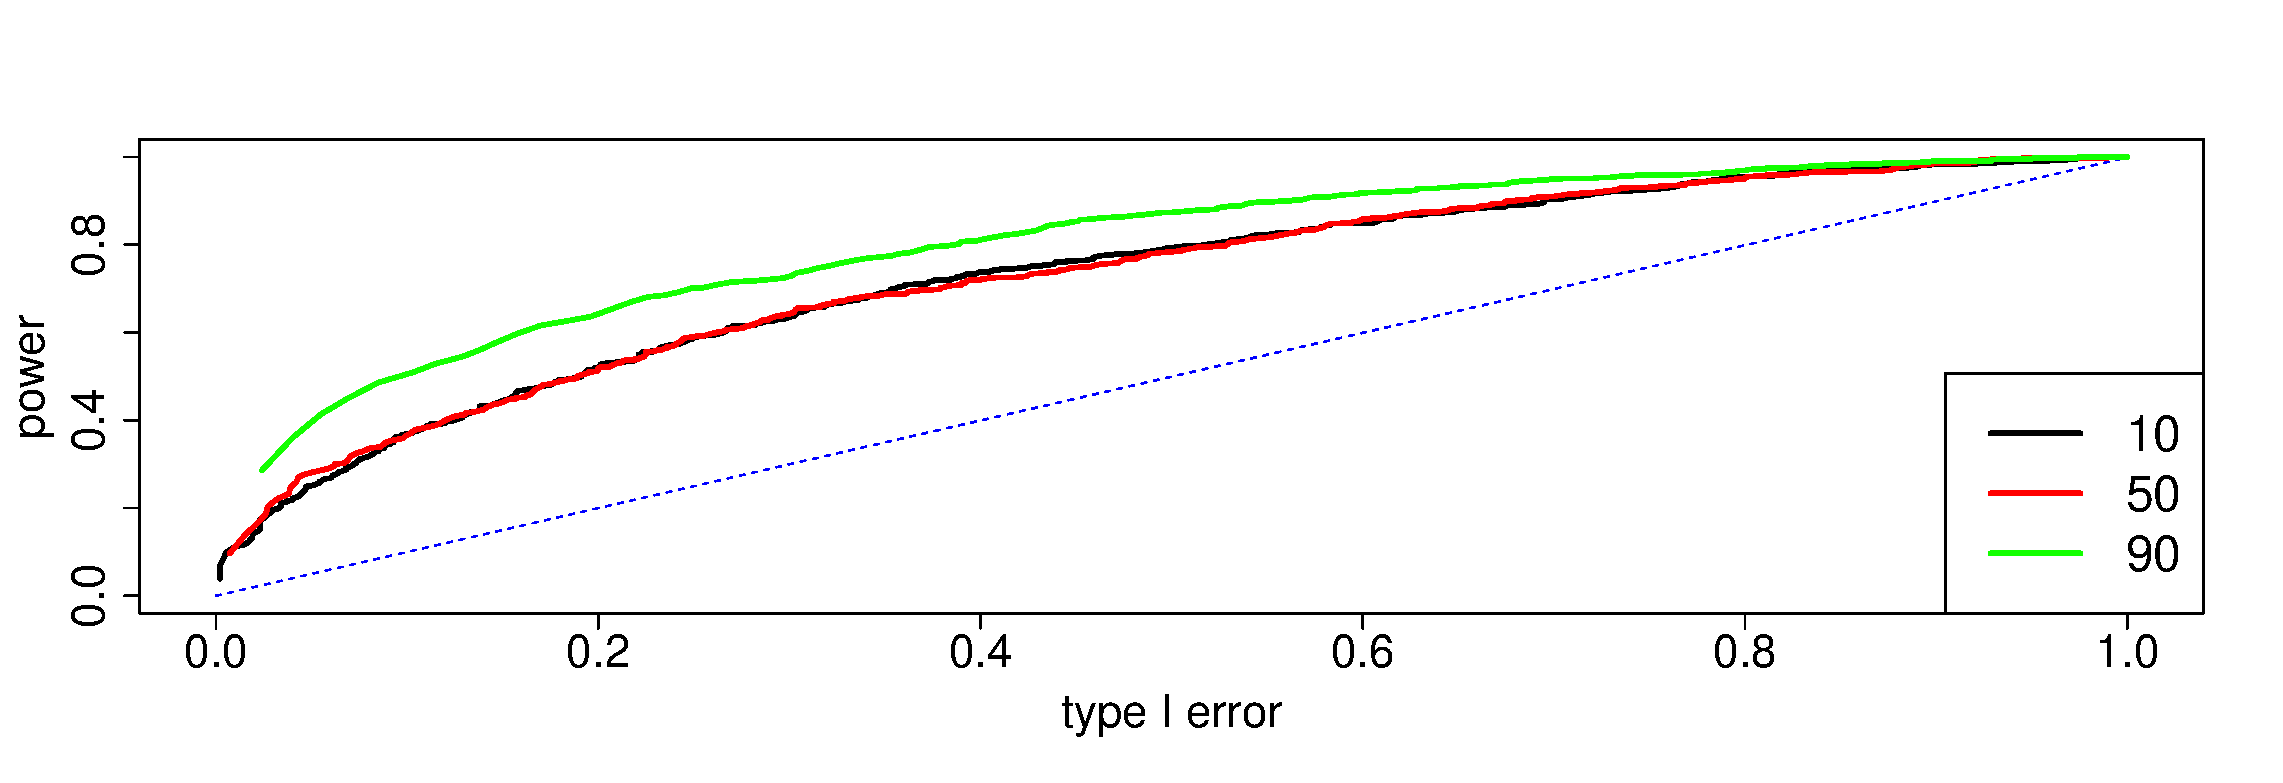
\includegraphics[width=0.7\textwidth]{../cps2024/images/roc_phi7_N100.eps}
			\caption{ROC-кривая ($\omega=0.075$)}
			\label{roc_phi7_N100}
		\end{subfigure}
	\label{fig:example1}
	\caption{Пример 1 ($\varphi=0.7$, $N=100$)}
	\end{figure}
	По графику ошибок первого рода на рис.~\ref{alphaI_phi7_N100} видно, что чем больше $L$, тем более радикальным становится критерий. На рис.~\ref{roc_phi7_N100} изображены ROC-кривые критериев, наибольшую мощность дает критерий с $L=90$. На этом примере видно, что самым мощным является самый радикальный критерий. 
\end{example}

\begin{example}\label{example2}
	Пусть $\varphi=0.3$, $N=100$.
	\begin{figure}[h!]
		\captionsetup[subfigure]{justification=Centering}
		\begin{subfigure}[t]{\textwidth}
			\centering
			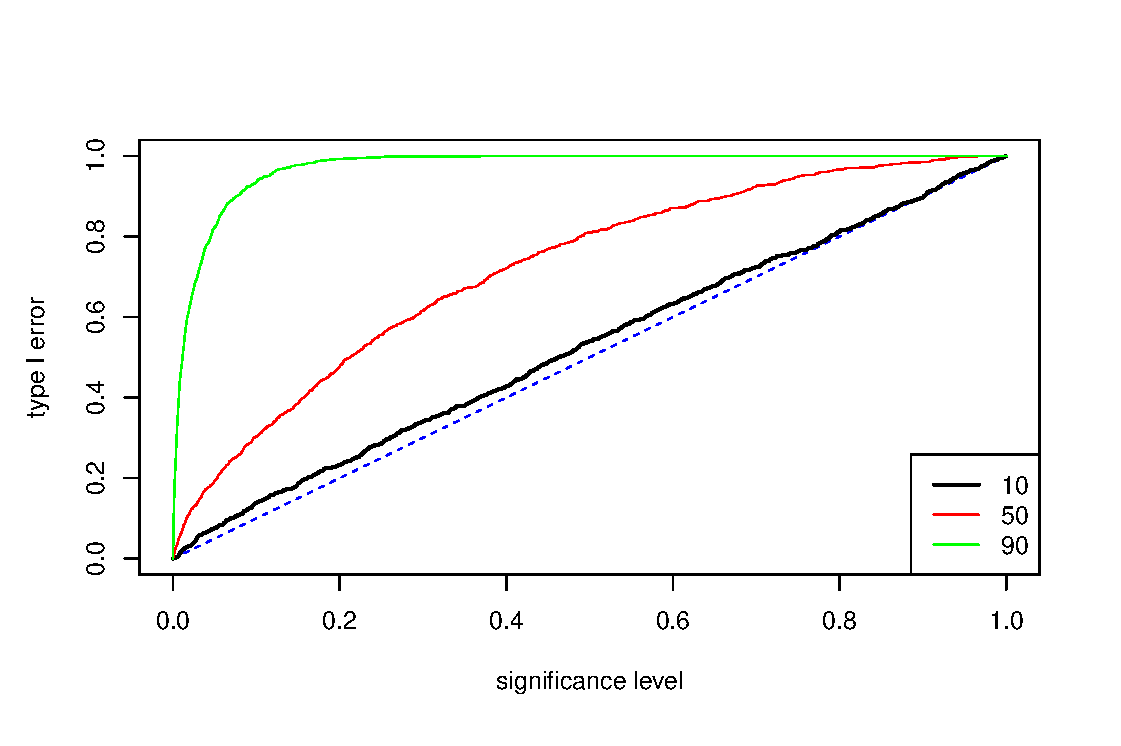
\includegraphics[width=0.7\textwidth]{../cps2024/images/alphaI_phi3_N100.eps}
			\caption{Ошибка I рода}
			\label{alphaI_phi3_N100}
		\end{subfigure}
		\begin{subfigure}[t]{\textwidth}
			\centering
			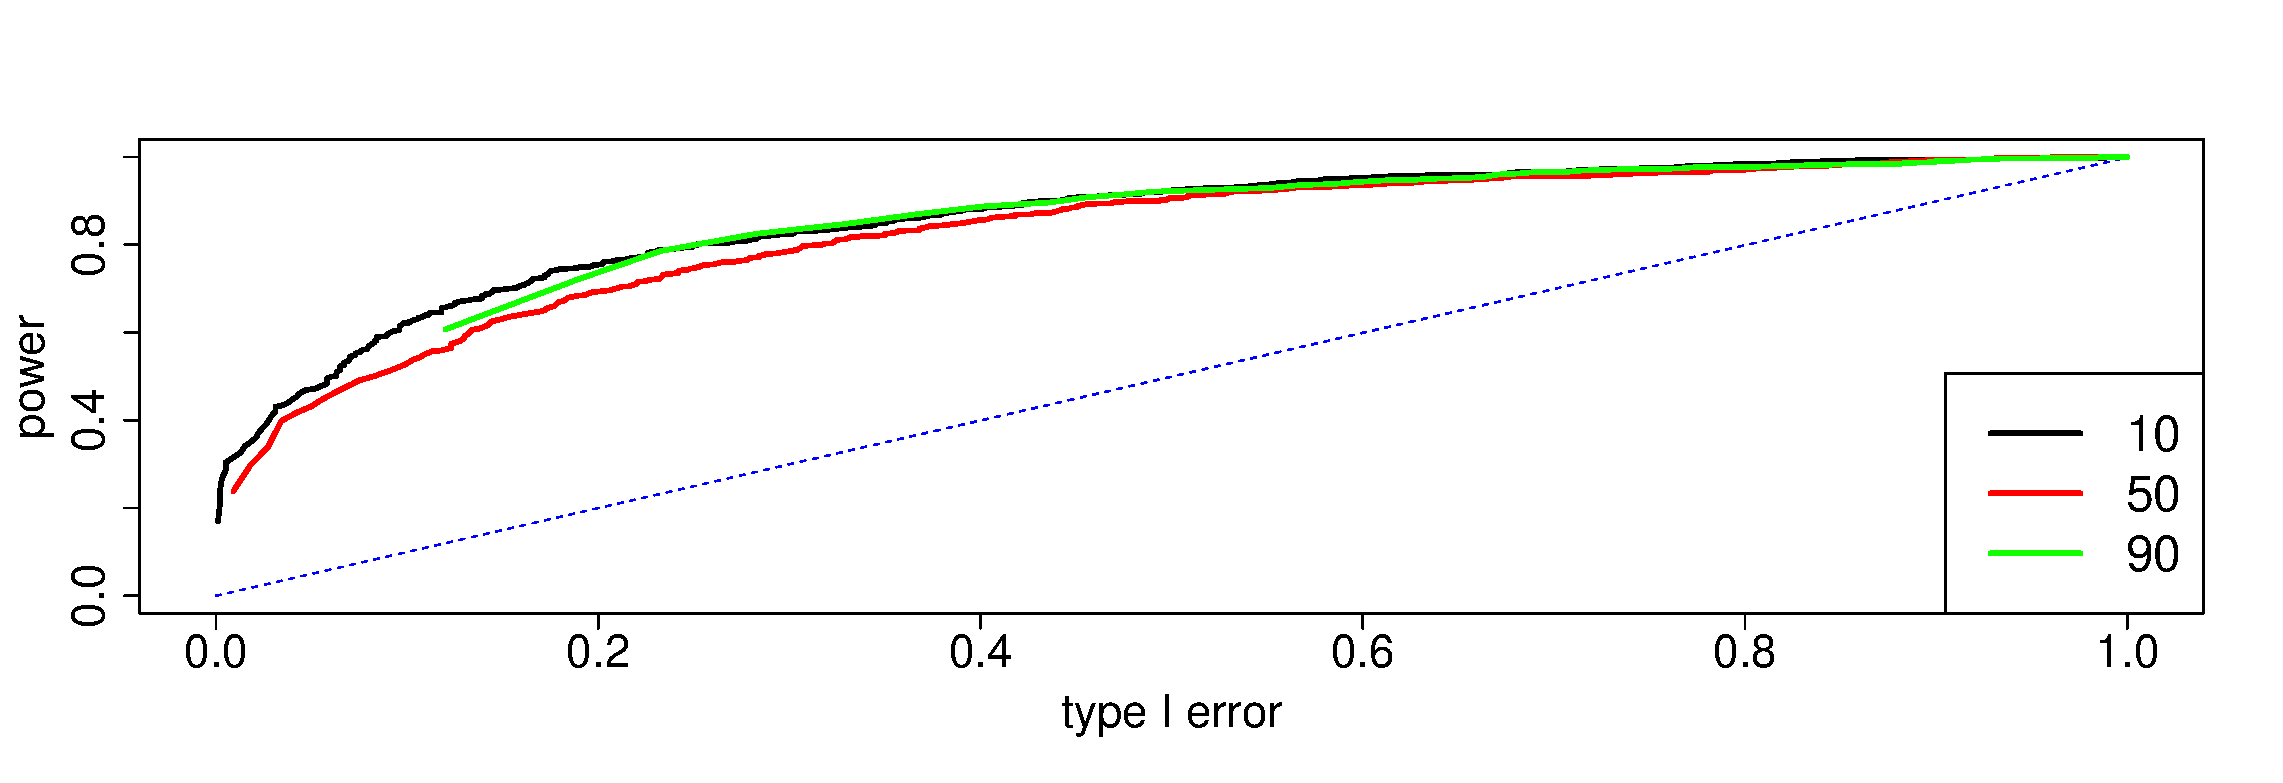
\includegraphics[width=0.7\textwidth]{../cps2024/images/roc_phi3_N100.eps}
			\caption{ROC-кривая ($\omega=0.075$)}
			\label{roc_phi3_N100}
		\end{subfigure}
	\label{fig:example2}
	\caption{Пример 2 ($\varphi=0.3$, $N=100$)}
	\end{figure}
	На рис.~\ref{alphaI_phi3_N100} изображен график ошибок первого рода. По нему видно, что, как и в примере 1, чем больше $L$, тем больше радикальность критерия. Если взглянуть на ROC-кривые на рис.~\ref{roc_phi3_N100}, то видно, что с уменьшением параметра $\varphi$ уменьшается разброс мощности критериев после поправки в зависимости от длины окна. Лучшей из рассмотренных в этом случае является $L=10$, хотя разница с $L=50$ совсем небольшая, а для $L=90$ для небольших ошибок I рода поправку сделать не удалось из-за радикальности.
\end{example}

Объяснить такое поведение радикальности в зависимости от длины окна $L$ можно теоретически: с увеличением $L$ увеличивается размер автоковариационной матрицы и тем самым увеличивается количество оцениваемых параметров, что влечет за собой большую подгонку собственных векторов к конкретной реализации шума.

\begin{example}\label{example3}
	Теперь увеличим длину ряда до $N=400$ и посмотрим на ROC-кривые для примеров~\ref{example1},~\ref{example2}.
	\begin{figure}[h!]
		\captionsetup[subfigure]{justification=Centering}
		\begin{subfigure}[t]{\textwidth}
			\centering
			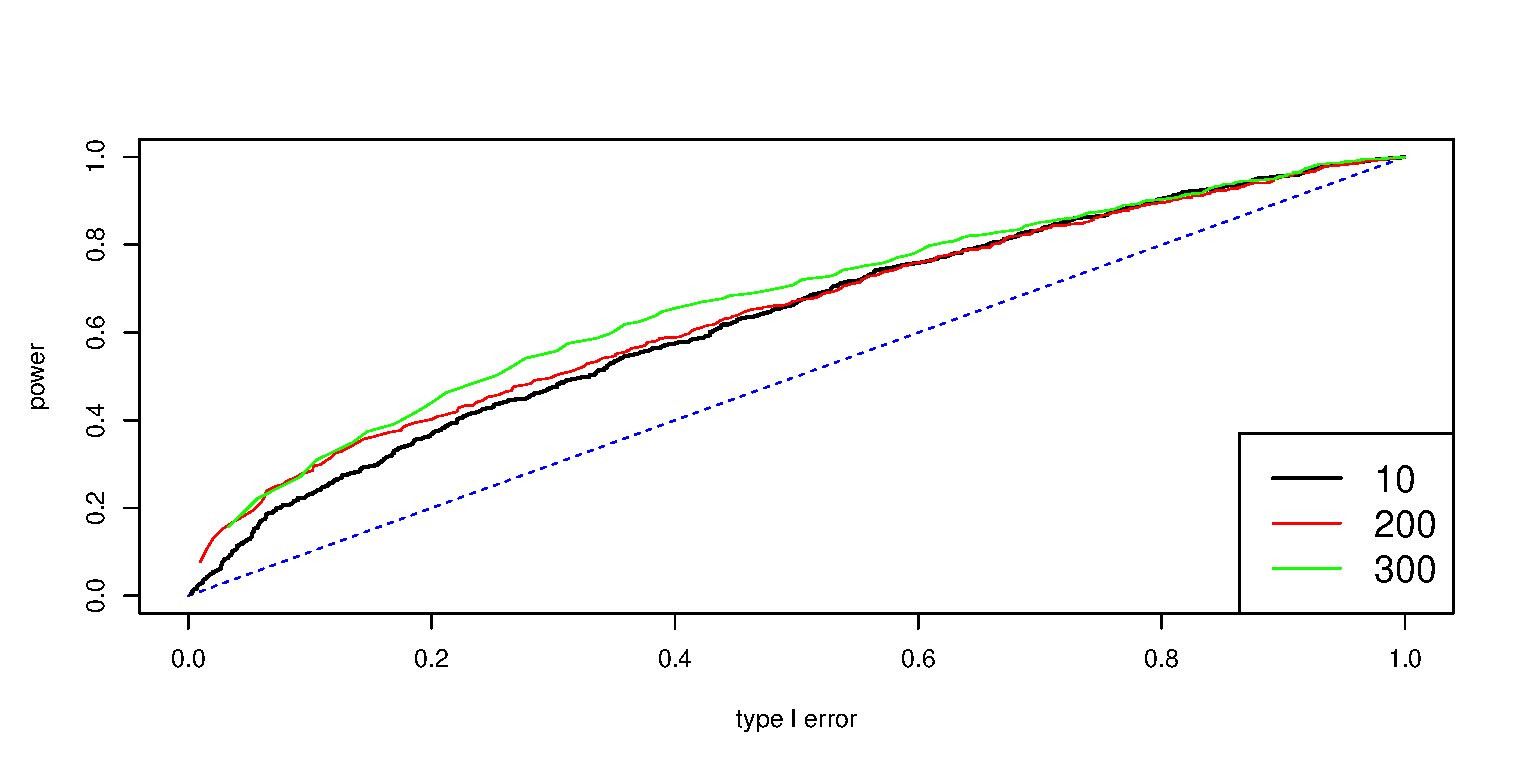
\includegraphics[width=0.7\textwidth]{../cps2024/images/roc_phi7_N400.eps}
			\caption{ROC-кривая ($\varphi=0.7$)}
			\label{roc_phi7_N400}
		\end{subfigure}
		\begin{subfigure}[t]{\textwidth}
			\centering
			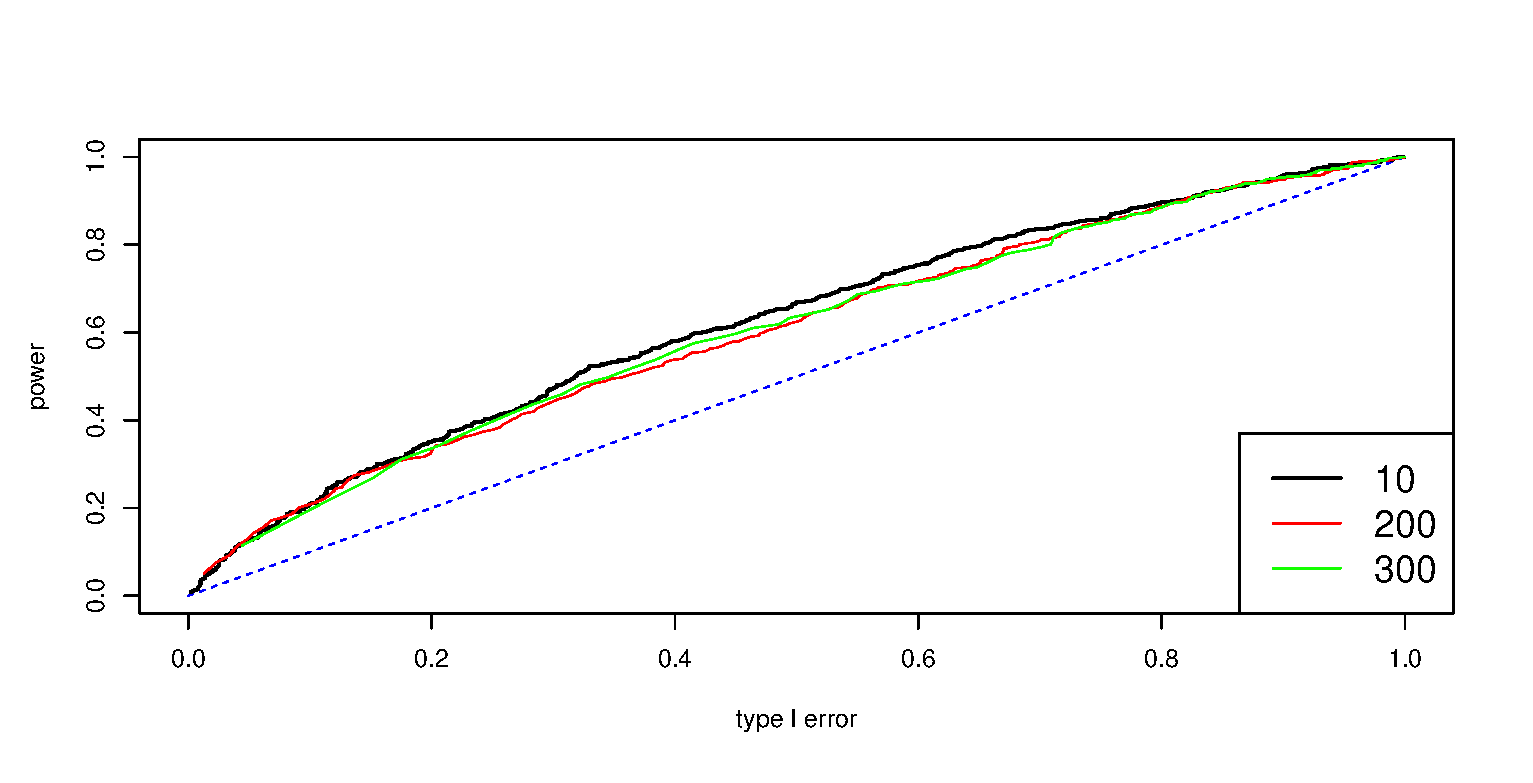
\includegraphics[width=0.7\textwidth]{../cps2024/images/roc_phi3_N400.eps}
			\caption{ROC-кривая ($\varphi=0.3$)}
			\label{roc_phi3_N400}
		\end{subfigure}
	\label{fig:example3}
	\caption{Пример 3 ($N=400$, $\omega=0.075$)}
	\end{figure}
	На рис.~\ref{roc_phi7_N400},~\ref{roc_phi3_N400} видим, что для обоих примеров с увеличением длины ряда уменьшается различие в мощности после поправки в зависимости от длины окна.
\end{example}

\begin{example}
	В условиях примера~\ref{example1} рассмотрим разные частоты $\omega$ сигнала $\tS$ и зависимость упорядоченности критериев по мощности от $L$. 
	\begin{figure}[h!]
		\captionsetup[subfigure]{justification=Centering}
		\begin{subfigure}[t]{\textwidth}
			\centering
			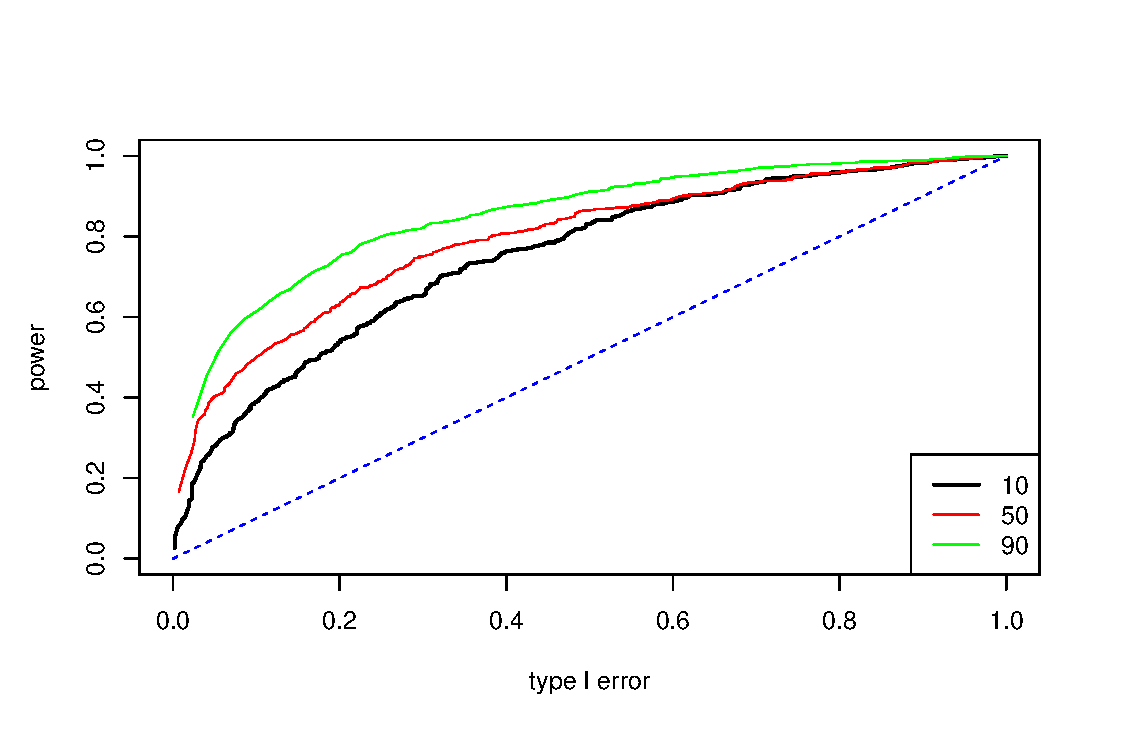
\includegraphics[width=0.7\textwidth]{../cps2024/images/roc_omega0175.eps}
			\caption{ROC-кривая ($\omega=0.175$)}
			\label{roc_omega0025}
		\end{subfigure}
		\begin{subfigure}[t]{\textwidth}
			\centering
			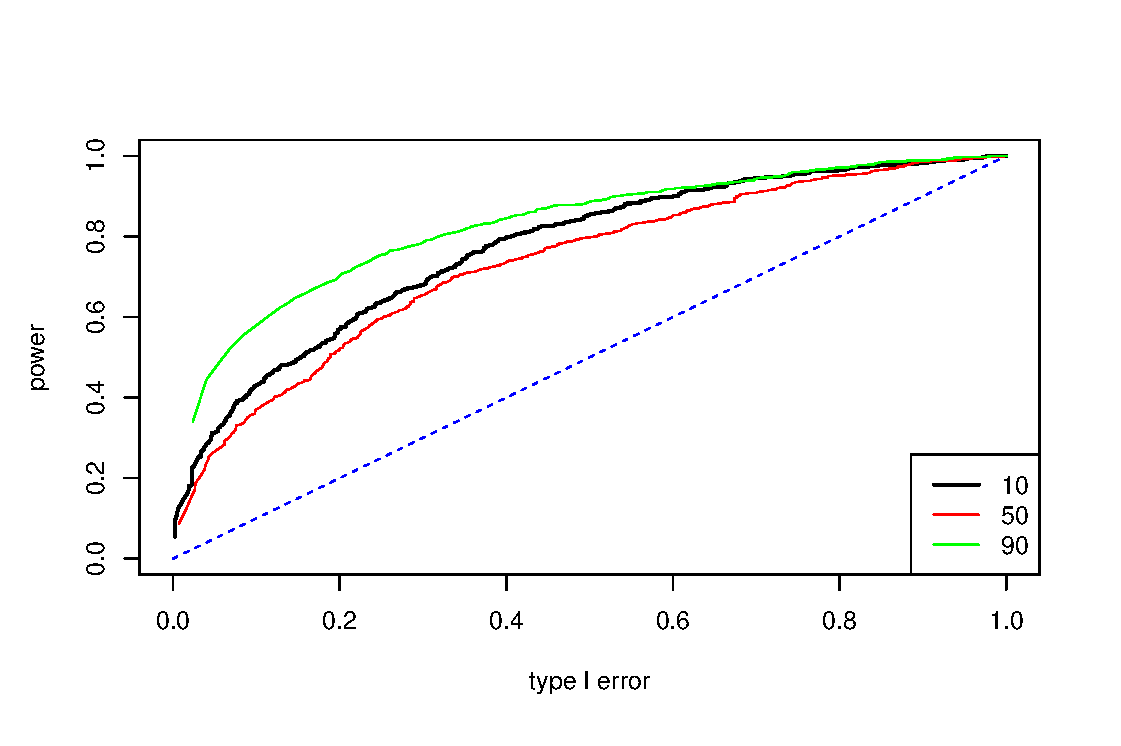
\includegraphics[width=0.7\textwidth]{../cps2024/images/roc_omega0025.eps}
			\caption{ROC-кривая ($\omega=0.025$)}
			\label{roc_omega0175}
		\end{subfigure}
	\label{fig:example4}
	\caption{Пример 4 ($\varphi=0.7$, $N=100$)}
	\end{figure}
	На рис.~\ref{roc_omega0175},~\ref{roc_omega0025} изображены ROC-кривые критериев при разных альтернативах. Видно, что упорядоченность $L$ нарушается при маленьких частотах сигнала. Если упорядочить рис.~\ref{roc_omega0175}, рис.~\ref{roc_phi7_N100} и рис.~\ref{roc_omega0025} по частоте $\omega$, то видна динамика по соотношению ROC-кривых для $L=10$ и $L=50$.
\end{example}

\begin{example}
	Рассмотрим $N=100$, $200$, $500$, $1000$ и посмотрим на графики ошибок I рода при разных $L$.
	\begin{figure}[h!]
		\captionsetup[subfigure]{justification=Centering}
		\begin{subfigure}[t]{\textwidth}
			\centering
			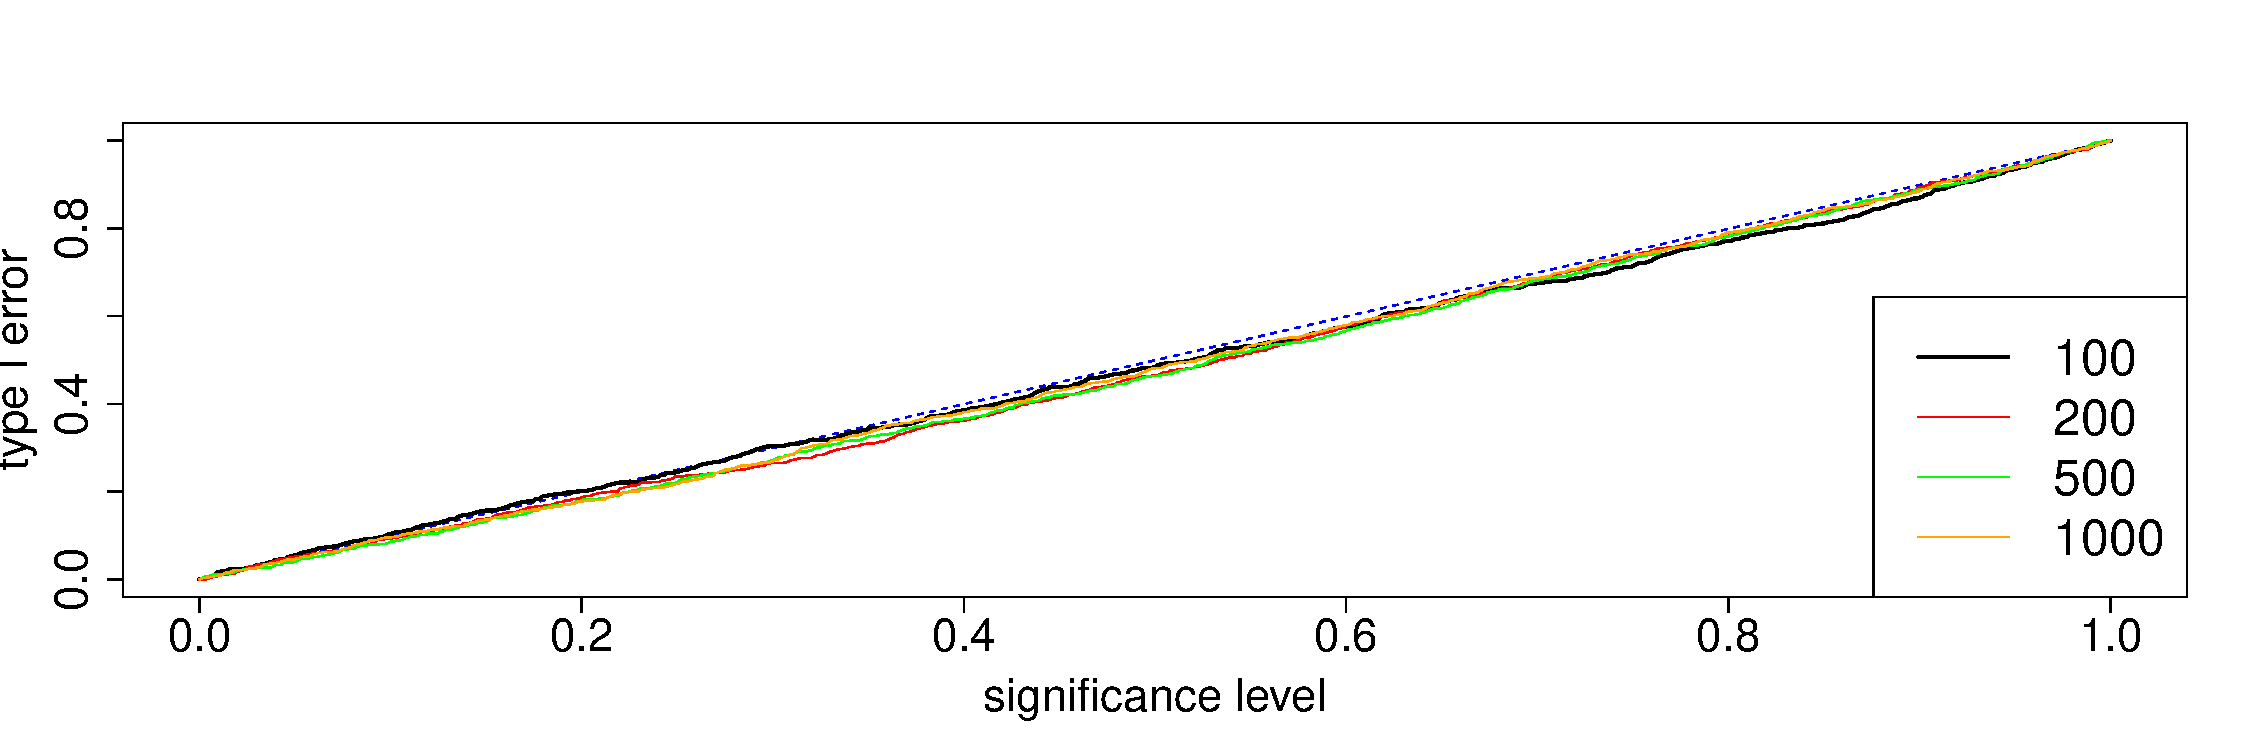
\includegraphics[width=0.7\textwidth]{img/alphaI_L10.pdf}
			\caption{Ошибка I рода ($L=10$)}
			\label{alphaI_L10}
		\end{subfigure}
		\begin{subfigure}[t]{\textwidth}
			\centering
			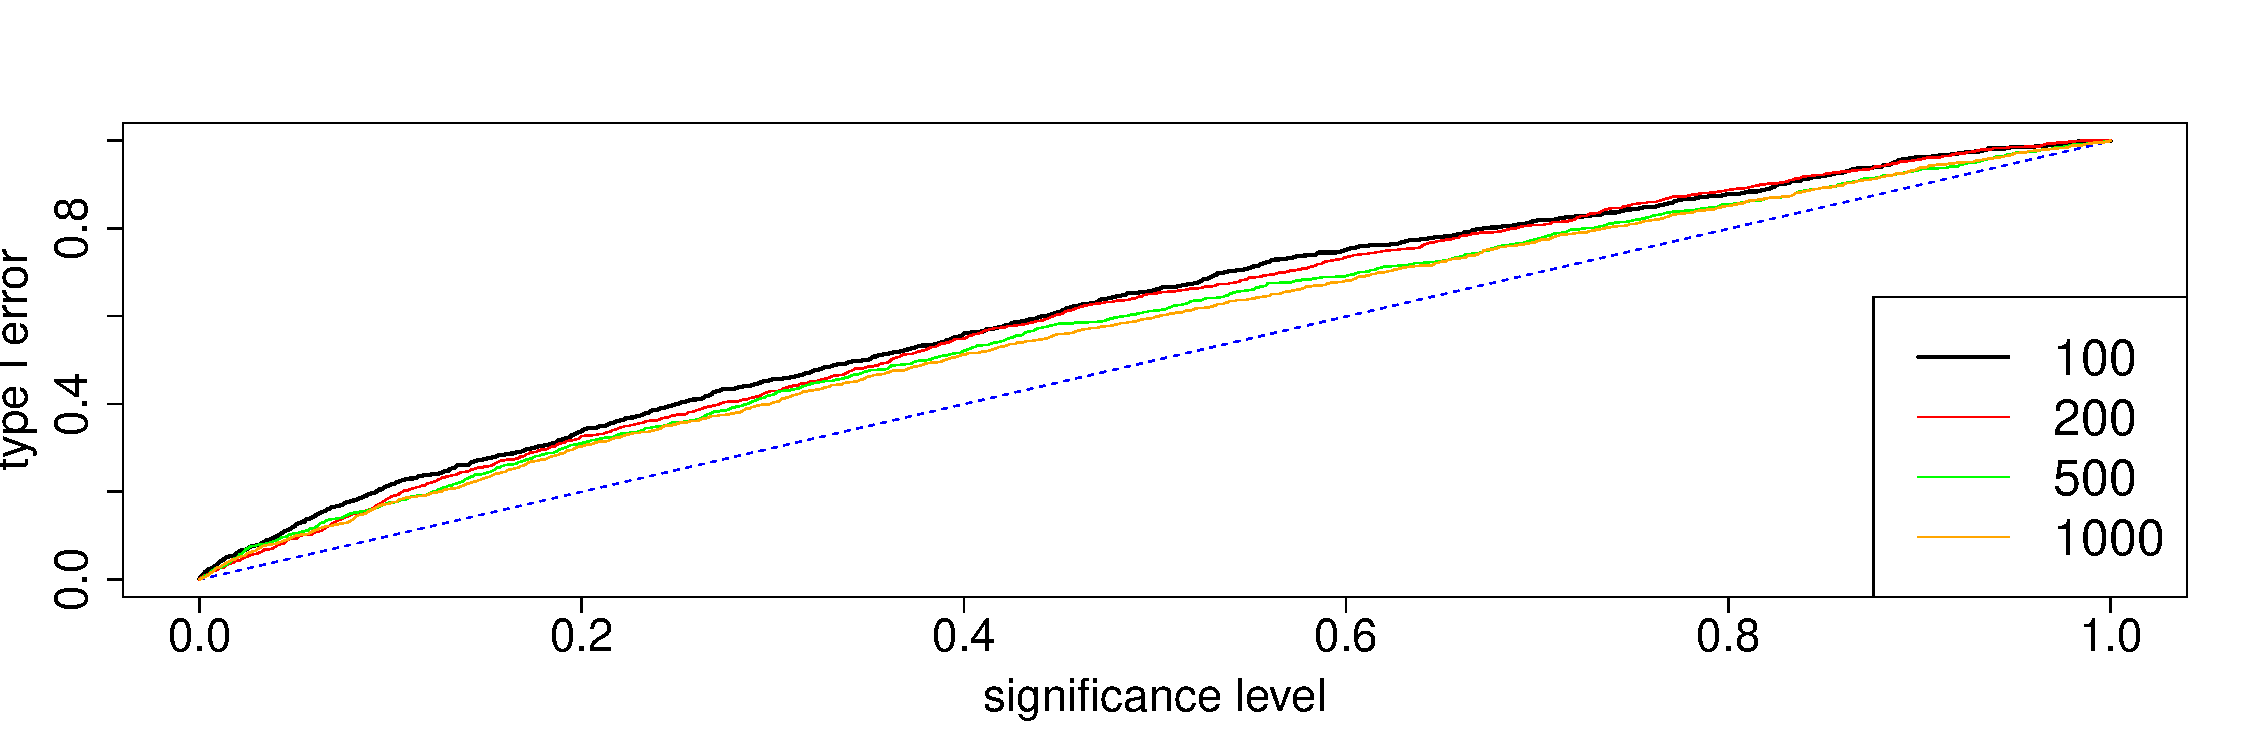
\includegraphics[width=0.7\textwidth]{img/alphaI_L40.pdf}
			\caption{Ошибка I рода ($L=40$)}
			\label{alphaI_L40}
		\end{subfigure}
	\label{fig:example5}
	\caption{Пример 5 (поведение ошибки первого рода в зависимости от длины ряда)}
	\end{figure}
	Из рис~\ref{alphaI_L10} видно, что критерий с $L=10$ примерно точный для всех $N$. На рис.~\ref{alphaI_L40} наблюдается очень медленное уменьшение радикальности критерия с ростом $N$.

\end{example}

Численные эксперименты показали, что длина окна $L$, дающая максимальную мощность критерия после поправки, зависит от параметров шума, длины ряда и, главное, от частоты сигнала в альтернативной гипотезе. Поэтому при выборе длины окна возможны следующие варианты:
\begin{enumerate}
	\item При больших $N$ применение поправки, описанной в разделе~\ref{sect:correction}, является трудоемкой задачей даже для небольших $L$. Также было замечено, что с ростом $N$ радикальность критерия при фиксированном $L$ едва заметно уменьшается. Поэтому из рассмотренных примеров получено, что без поправки можно использовать MC-SSA только с $L=10$. Это нетрудозатратно, но возможна некоторая потеря в мощности. Но, поскольку с увеличением длины ряда уменьшается различие в мощности в зависимости от длины окна, для больших $N$ эта потеря будет не такая заметная.
	\item В поведении оптимальной по мощности длины окна $L$ в зависимости от параметров ряда наблюдается некоторая регулярность. Поэтому можно построить зависимость оптимальной длины окна от параметров ряда с помощью численного моделирования, оценив параметры красного шума. Однако было показано, что упорядоченность критериев по мощности зависит от частоты сигнала в альтернативе, поэтому эта рекомендация имеет практический смысл, только если есть дополнительная информация о диапазоне возможных частот в альтернативе.
\end{enumerate}

\section{Оценка параметров красного шума}\label{sect:phi_est}
До сих пор мы предполагали, что параметры красного шума $\varphi$ и $\delta$ известны, но в реальных задачах редко возникает такая ситуация. В этой ситуации можно воспользоваться методом bootstrapping, который позволяет использовать оцененные параметры шума для построения критерия~\cite{Golyandina_2023}. Рассмотрим два способа оценивания неизвестных параметров $\varphi$ и $\delta$:
\begin{enumerate}
	\item Оценка параметров на основе исходного ряда методом максимального правдоподобия, где для нахождения начальных значений используется метод CSS~\cite{ARIMA_est}.
	\item Двухступенчатая оценка параметров, предлагаемая в этой работе:
	\begin{enumerate}
		\item[a)] Находится ОМП на основе исходного ряда;
		\item[b)] Применяется MC-SSA с поправкой;
		\item[c)] Если сигнал обнаруживается, он выделяется;
		\item[d)] Находится ОМП на основе <<остатка>>.
	\end{enumerate}
\end{enumerate}
%Двухступенчатая оценка точнее оценивает неизвестные параметры и увеличивает мощность MC-SSA, если верна $H_1$.

Проверим на практике, что двухступенчатая оценка параметров даст результаты лучше, чем обычная без выделения сигнала. За альтернативу возьмем
\begin{equation}\label{eq:noise_est_h1}
s_n=A\cos(2\pi\omega n),\quad n=1,\ldots,N,
\end{equation}
с амплитудой $A=1.5$ и частотой $\omega\in(0,0.5)$. Пусть $N=100$, $\varphi=0.7$, $\delta=1$. Для двухступенчатой оценки длина окна $\widetilde L=50$, $G=1000$, $\alpha=0.1$

Будем оценивать параметр $\varphi$, обозначим оценку за $\hat\varphi$. В качестве оценки точности было взято среднеквадратичное отклонение от истинного значения. В таблице~\ref{tab:param_estim} представлены результаты на основе 100 реализаций шума. Поскольку $\mathsf{MSE}\hat\varphi=\mathsf{D}\hat\varphi + \mathsf{bias}^2\hat\varphi$, в таблице также представлены значения дисперсии и смещения оценки.

\begin{table}[h]
	\centering
	\begin{tabular}{|cccccc|}
		\hline
		Обычная оценка & $\omega = 0.075$ & $\omega=0.175$ & $\omega=0.275$ & $\omega=0.375$ & $\omega=0.475$ \\
		\hline
		$\mathsf{MSE}\hat\varphi$ & $0.0053$ & $0.0124$ & $0.1185$ & $0.3109$ & $0.4018$ \\
		\hline
		$\mathsf{D}\hat\varphi$ & $0.0023$ & $0.0036$ & $0.007$ & $0.0189$ & $0.0204$ \\
		\hline
		$\mathsf{bias}\hat\varphi$ & $0.055$ & $-0.0938$ & $-0.3341$ & $-0.5406$ & $-0.6178$\\
		\hhline{======}
		Двухступенчатая оценка & $\omega = 0.075$ & $\omega=0.175$ & $\omega=0.275$ & $\omega=0.375$ & $\omega=0.475$ \\
		\hline
		$\mathsf{MSE}\hat\varphi$ & $0.0091$ & $0.0057$ & $0.0038$ & $0.0098$ & $0.0129$ \\
		\hline
		$\mathsf{D}\hat\varphi$ & $0.0084$ & $0.0056$ & $0.0037$ & $0.0085$ & $0.0101$ \\
		\hline
		$\mathsf{bias}\hat\varphi$ & $-0.0284$ & $-0.0119$ & $-0.0107$ & $-0.0375$ & $-0.0538$\\
		\hline
	\end{tabular}
	\caption{Оценка параметров красного шума ($\varphi=0.7$)}
	\label{tab:param_estim}
\end{table}

По таблице~\ref{tab:param_estim} видно, что основной вклад в ошибку оценки вносит смещение, описанная выше процедура это смещение сильно уменьшает, делая слабо-отрицательным.
\begin{remark}
	В таблице~\ref{tab:param_estim} были взяты такие $\omega$ с целью показать общий случай, поскольку если $\widetilde L\omega$ "--- целое, то SSA точнее выделяет сигнал~\cite{ssa_an} и, следовательно, сделает оценку параметров лучше.
\end{remark}

Теперь сравним графики ошибок первого рода и ROC-кривые критерия MC-SSA против альтернативы~\eqref{eq:noise_est_h1} с $\omega=0.075$. Длины окна $L$ будем брать те же, что и в разделе~\ref{mc-mssa_numeric_comparison}.

\begin{figure}[h!]
	\captionsetup[subfigure]{justification=Centering}
	\begin{subfigure}[t]{0.5\textwidth}
		\centering
		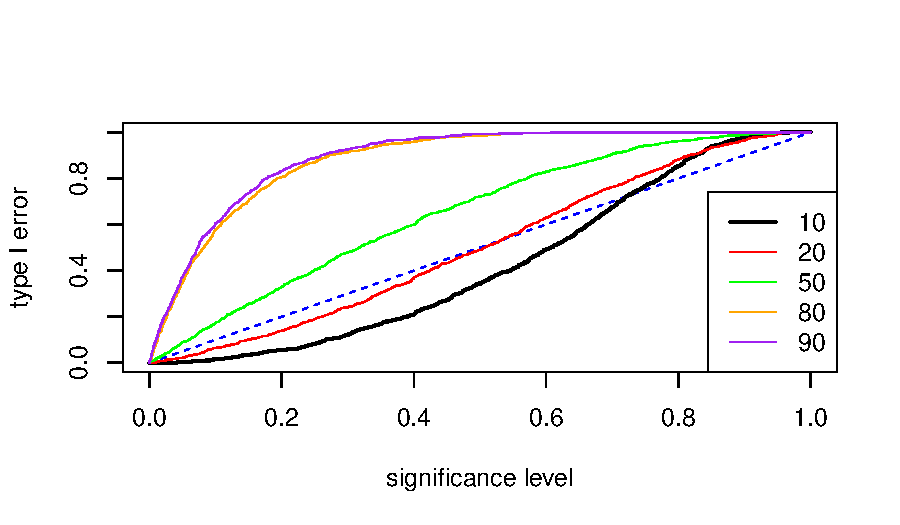
\includegraphics[width=0.95\textwidth]{img/type1error_arima.pdf}
		\caption{Ошибка первого рода (обычная оценка)}
		\label{fig:arima_type1error}
	\end{subfigure}\hspace{\fill}
	\begin{subfigure}[t]{0.5\textwidth}
		\centering
		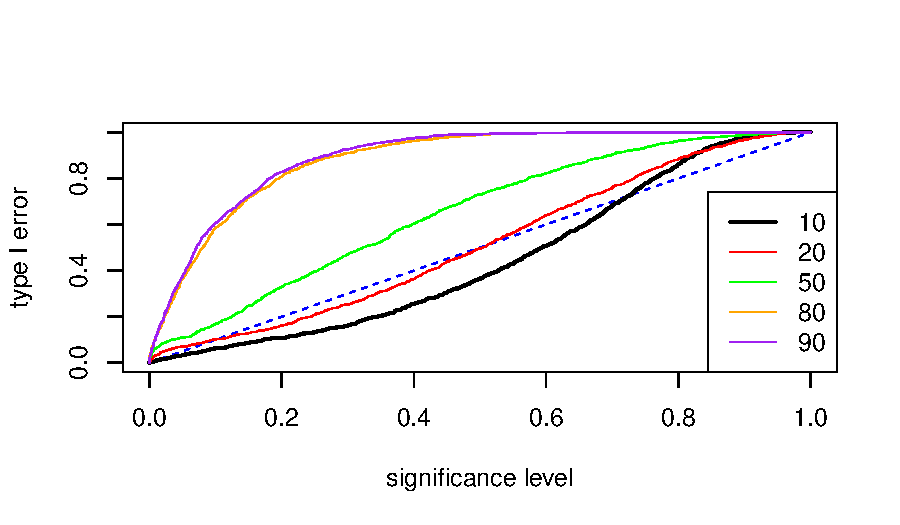
\includegraphics[width=0.95\textwidth]{img/type1error_extract.pdf}
		\caption{Ошибка первого рода (двухступенчатая оценка)}
		\label{fig:extract_type1error}
	\end{subfigure}
	\bigskip
	\begin{subfigure}[t]{0.5\textwidth}
		\centering
		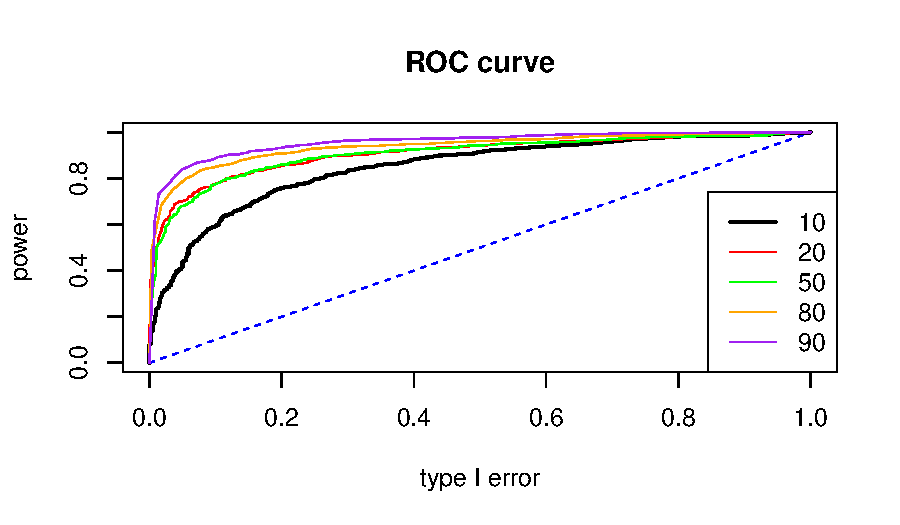
\includegraphics[width=0.95\textwidth]{img/roc_arima.pdf}
		\caption{ROC-кривая (обычная оценка)}
		\label{fig:arima_roc}
	\end{subfigure}\hspace{\fill}
	\begin{subfigure}[t]{0.5\textwidth}
		\centering
		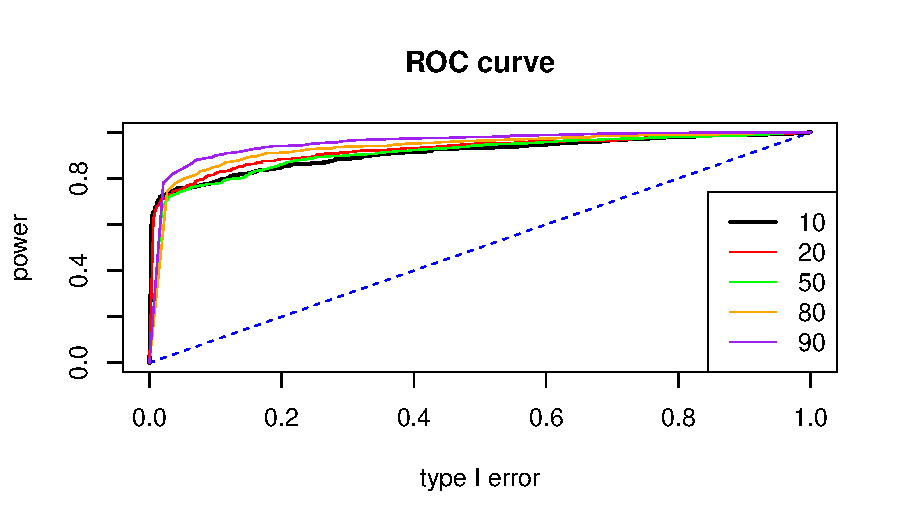
\includegraphics[width=0.95\textwidth]{img/roc_extract.pdf}
		\caption{ROC-кривая (двухступенчатая оценка)}
		\label{fig:extract_roc}
	\end{subfigure}
	\caption{Сравнение обычной и двухступенчатой оценок}
\end{figure}

По рис.~\ref{fig:arima_type1error} и~\ref{fig:extract_type1error} видно, графики ошибок первого рода примерно одинаковые для всех длин окна, что естественно, поскольку сигнала нет, и, следовательно, оценки параметров приблизительно одинаковые. А если посмотреть на ROC-кривые на рис.~\ref{fig:arima_roc} и~\ref{fig:extract_roc}, заметно повышение мощности при $L=10$, $20$, $50$. 

Хотя при маленьких длинах окна двухступенчатая оценка увеличивает мощность, что полезно при применении MC-SSA к рядам большой длины, использовать эту процедуру можно, если известно точно, что значимые компоненты являются сигналом, а не следствием неправильной модели. Поэтому в дальнейшем будем оценивать параметры обычным, не двухступенчатым, образом.
%Поскольку для оптимальной длины окна $L=90$ разницы в мощности нет, и для рядов большой длины применение поправки численно трудоемкая задача, далее будем оценивать параметры шума обычным, не двухступенчатым, способом.

\section{Наличие мешающего сигнала}\label{sect:nuisance}
Пусть известно, что во временном ряде присутствует некоторый сигнал, но, возможно, еще есть какой-то другой. Тогда модель выглядит следующим образом:
\[
\tX=\tF + \tS + \bfxi,
\]
где $\tF$ "--- мешающий сигнал, $\tS$ "--- неизвестный сигнал и $\bfxi$ "--- красный шум.
Тогда проверяется следующая нулевая гипотеза с альтернативой:
\begin{align*}
&H_0: \tS=0,\\
&H_1: \tS \ne 0.
\end{align*}
\begin{algorithm}{MC-SSA с мешающим сигналом}\label{mc-ssa_nuisance}
\begin{enumerate}
	\item Находится приближенное значение мешающего сигнала $\hat{\tF}$ и оцениваются параметры $\bfxi$ на основе остатка $\tilde\tX=\tX-\hat{\tF}$.
	\item Находятся левые векторы $P_1,\ldots,P_L$ траекторной матрицы временного ряда $\tilde\tX$, полученные из разложения~\eqref{eq:sum_decomposition}. 
	\item Применяется MC-SSA к исходному ряду $\tX$ с проекцией на векторы $P_1,\ldots,P_L$, при этом суррогатными рядами являются реализации случайной величины $\boldsymbol{\eta}$:
	\[
	\boldsymbol{\eta} = \bfxi + \hat\tF.
	\]
\end{enumerate}
\end{algorithm}
Цель данной модификации алгоритма "--- устранить влияние мешающего сигнала на вектора, на которые делается проекция.

Рассмотрим два примера мешающего сигнала, для которых будем рассматривать следующую альтернативу:
\[
	H_1: \tS = \{\cos(2\pi\omega n)\}_{n=1}^N,
\]
где $\omega=0.075$. Параметры красного шума и длину ряда $N$ возьмем такими же, как в разделе~\ref{sect:phi_est}: $\varphi=0.7$, $\delta=1$, $N=100$. 
\subsection{Периодическая компонента}\label{sect:periodic_case}
Рассмотрим в качестве мешающего сигнала синусоиду
\[
f_n=A\cos(2\pi\omega n),\quad n=1,\ldots,N,
\]
с амплитудой $A=3$ и частотой $\omega=0.25$.

Будем выделять периодическую компоненту при помощи SSA: будем оценивать доминирующую частоту левых векторов с помощью метода \textsf{ESPRIT}~\cite[Раздел 3.1]{SSA_R} и на шаге группировки (раздел~\ref{sect:grouping}) будем брать две компоненты с наиболее близкими к $\omega$ частотами. 
\begin{figure}[h!]
	\captionsetup[subfigure]{justification=Centering}
	\begin{subfigure}[t]{0.5\textwidth}
		\centering
		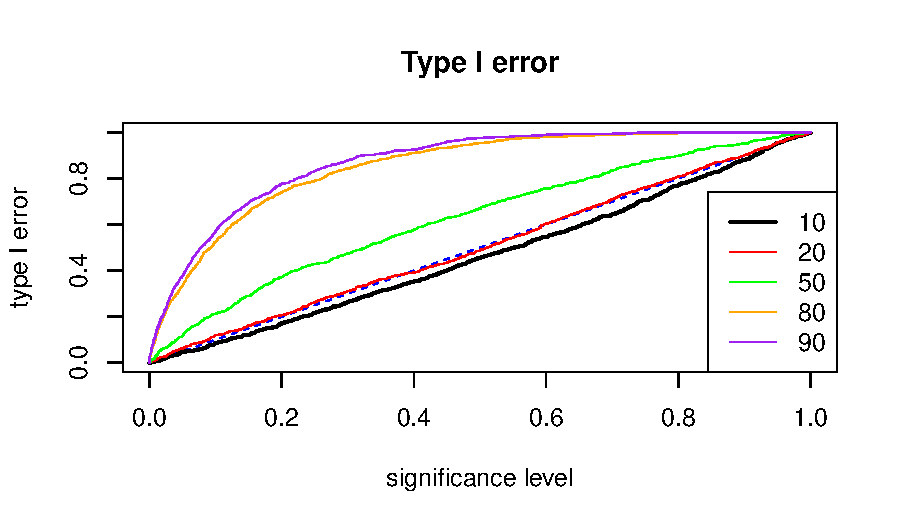
\includegraphics[width=0.95\textwidth]{img/type1error_sin.pdf}
		\caption{Ошибка I рода}
		\label{fig:sin_type1error}
	\end{subfigure}\hspace{\fill}
	\begin{subfigure}[t]{0.5\textwidth}
		\centering
		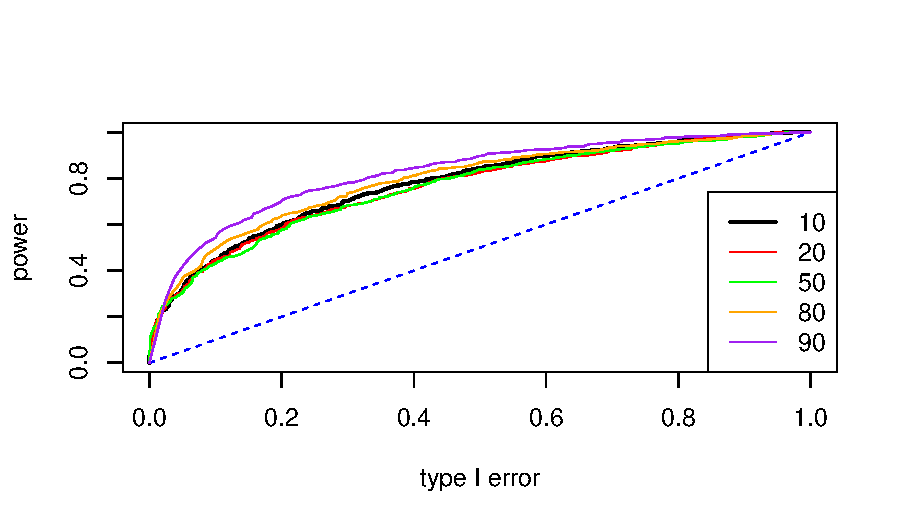
\includegraphics[width=0.95\textwidth]{img/roc_sin.pdf}	
		\caption{ROC-кривая}
		\label{fig:sin_roc}
	\end{subfigure}
	\begin{subfigure}[t]{0.5\textwidth}
		\centering
		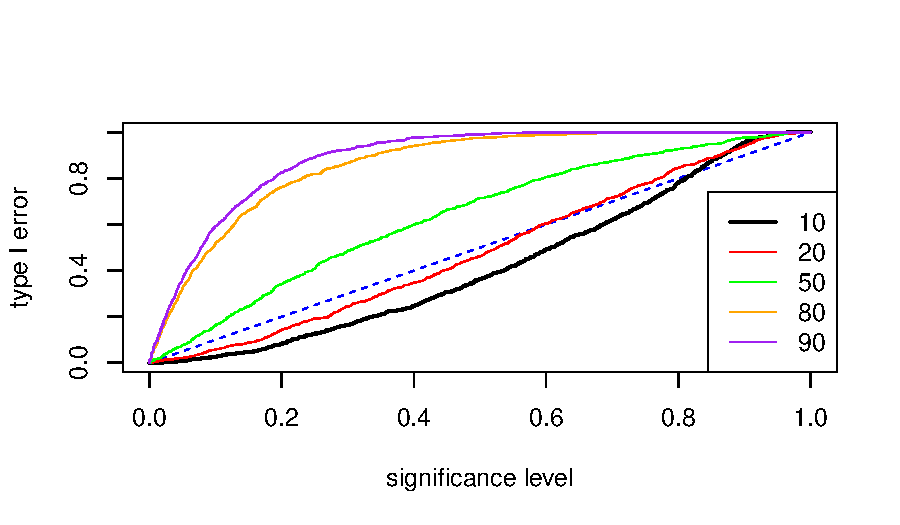
\includegraphics[width=0.95\textwidth]{img/type1error_sin_est_noise.pdf}
		\caption{Ошибка I рода (оцененные параметры шума)}
		\label{fig:sin_est_noise_type1error}
	\end{subfigure}\hspace{\fill}
	\begin{subfigure}[t]{0.5\textwidth}
		\centering
		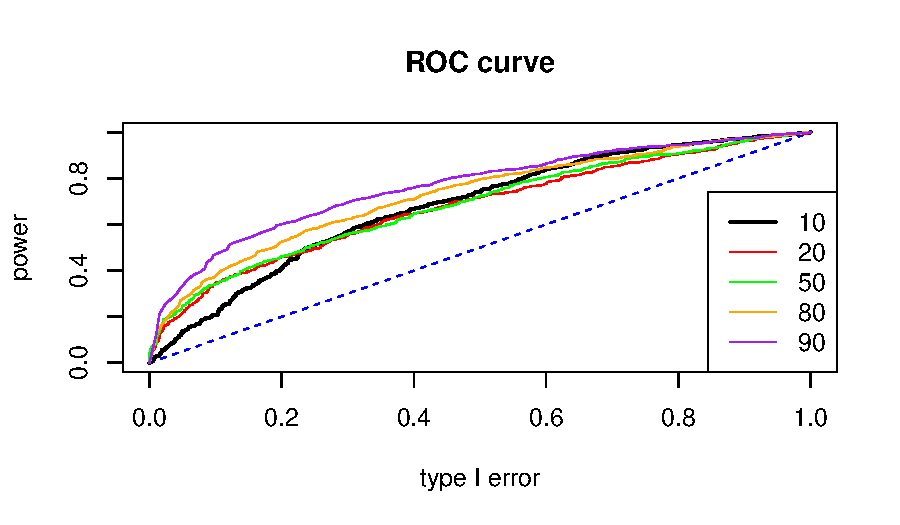
\includegraphics[width=0.95\textwidth]{img/roc_sin_est_noise.pdf}
		\caption{ROC-кривая (оцененные параметры шума)}
		\label{fig:sin_est_noise_roc}
	\end{subfigure}
	\begin{subfigure}[t]{0.5\textwidth}
		\centering
		\includegraphics[width=0.95\textwidth]{img/type1error_sin_est_noise_signal.pdf}
		\caption{Ошибка I рода (оцененный мешающий сигнал и параметры шума)}
		\label{fig:sin_est_noise_signal_type1error}
	\end{subfigure}\hspace{\fill}
	\begin{subfigure}[t]{0.5\textwidth}
		\centering
		\includegraphics[width=0.95\textwidth]{img/roc_sin_est_noise_signal.pdf}
		\caption{ROC-кривая (оцененный мешающий сигнал и параметры шума)}
		\label{fig:sin_est_noise_signal_roc}
	\end{subfigure}
	
	
	%\begin{subfigure}[t]{\textwidth}
	%	\centering
	%	\includegraphics[width=0.7\textwidth]{img/power_sin.pdf}
	%	\caption{Мощность}
	%	\label{fig:sin_power}
	%\end{subfigure}
	\caption{Анализ метода, когда мешающий сигнал "--- периодическая компонента}
	\label{fig:sin}
\end{figure}

На рис.~\ref{fig:sin} представлены графики ошибок первого рода и ROC-кривые следующих критериев: когда мешающий сигнал и параметры шума известны точно, когда $\tF$ известен точно, но параметры шума оцениваются, и когда и мешающий сигнал, и параметры шума оцениваются. Графики ошибок первого рода на рис.~\ref{fig:sin_type1error},~\ref{fig:sin_est_noise_type1error} и~\ref{fig:sin_est_noise_signal_type1error} похожи друг на друга, а отклонение от случая, когда все известно, можно объяснить погрешностью при оценке неизвестных параметров. После применения поправки из раздела~\ref{sect:correction} критерии становятся точными для любой длины окна и ROC-кривые на рис.~\ref{fig:sin_roc},~\ref{fig:sin_est_noise_roc} и~\ref{fig:sin_est_noise_signal_roc} представляют собой графики мощности этих критериев. Таким образом, наибольшая мощность во всех трех случаях достигается при $L=90$.
\begin{figure}[h!]
	\centering
	\includegraphics[width=0.7\textwidth]{img/roc_sin_copm.pdf}
	\caption{Сравнение ROC-кривых критериев (мешающий сигнал "--- периодическая компонента)}
	\label{fig:power_comp_sin}
\end{figure}

На рис.~\ref{fig:power_comp_sin} представлена ROC-кривая критериев для оптимального $L$. Как видно из графика, при оценке параметров шума и мешающего сигнала мощность падает, но незначительно (примерно на 10\%), что важно при применении алгоритма на практике.
%Будем смотреть на графики ошибки первого рода, мощности и ROC-кривые этого критерия для разных длин окна, как в разделе~\ref{mc-ssa_numeric_comparison}. Начнем с ситуации, когда сигнал и параметры шума известны точно, постепенно приходя к случаю, когда и сигнал, и параметры шума нужно оценивать. 


%На рис.~\ref{fig:sin} представлены графики ошибки первого рода, мощности и ROC-кривые критерия, когда сигнал и параметры шума известны точно. График ошибки первого рода на рис.~\ref{fig:sin_type1error} показывает, что при длине окна $L=10$ критерий консервативный, при $L=20$ "--- приблизительно точный, при остальных $L$ "--- радикальный. Таким образом, имеет смысл рассматривать мощность на рис.~\ref{fig:sin_power} только для $L=10,20$. ROC-кривая на рис.~\ref{fig:sin_roc} похожа на график мощности при $L=20$, что соответствует теории. После применения поправки наибольшая мощность достигается при длине окна $L=90$.

%\begin{figure}[h!]
%	\captionsetup[subfigure]{justification=Centering}
%	\begin{subfigure}[t]{\textwidth}
%		\centering
%		\includegraphics[width=0.7\textwidth]{img/type1error_sin_est_noise.pdf}
%		\caption{Ошибка первого рода}
%		\label{fig:sin_est_noise_type1error}
%	\end{subfigure}
%	\begin{subfigure}[t]{\textwidth}
%		\centering
%		\includegraphics[width=0.7\textwidth]{img/power_sin_est_noise.pdf}
%		\caption{Мощность}
%		\label{fig:sin_est_noise_power}
%	\end{subfigure}
%	\begin{subfigure}[t]{\textwidth}
%		\centering
%		\includegraphics[width=0.7\linewidth]{img/roc_sin_est_noise.pdf}
%		\caption{ROC-кривая}
%		\label{fig:sin_est_noise_roc}
%	\end{subfigure}
%	\caption{Анализ метода с оцененными параметрами шума (сигнал "--- периодическая компонента)}
%	\label{fig:sin_est_noise}
%\end{figure}

%На рис.~\ref{fig:sin_est_noise} представлены графики ошибки первого рода, мощности и ROC-кривые критерия, когда сигнал известен точно, но параметры шума оцениваются. График ошибки первого рода на рис.~\ref{fig:sin_est_noise_type1error} показывает, что при длине окна $L=10$ при $\alpha<0.82$ и $L=20$ при $\alpha<0.58$ критерий консервативный, в иных случаях --- радикальный. Таким образом, имеет смысл рассматривать мощность на рис.~\ref{fig:sin_est_noise_power} только для $L=10$ при $\alpha<0.82$ и $L=20$ при $\alpha<0.58$. Наибольшая мощность поправленного критерия достигается при длине окна $L=90$. Отклонение от случая с известным сигналом и параметрами шума можно объяснить погрешностями при оценке параметров.
%\begin{figure}[h!]
%	\captionsetup[subfigure]{justification=Centering}
%	\begin{subfigure}[t]{\textwidth}
%		\centering
%		\includegraphics[width=0.7\textwidth]{img/type1error_sin_est_noise_signal.pdf}
%		\caption{Ошибка первого рода}
%		\label{fig:sin_est_noise_signal_type1error}
%	\end{subfigure}
%	\begin{subfigure}[t]{\textwidth}
%		\centering
%		\includegraphics[width=0.7\textwidth]{img/power_sin_est_noise_signal.pdf}
%		\caption{Мощность}
%		\label{fig:sin_est_noise_signal_power}
%	\end{subfigure}
%	\begin{subfigure}[t]{\textwidth}
%		\centering
%		\includegraphics[width=0.7\linewidth]{img/roc_sin_est_noise_signal.pdf}
%		\caption{ROC-кривая}
%		\label{fig:sin_est_noise_signal_roc}
%	\end{subfigure}
%	\caption{Анализ метода с оцененным сигналом и параметрами шума (сигнал "--- периодическая компонента)}
%	\label{fig:sin_est_noise_signal}
%\end{figure}

%На рис.~\ref{fig:sin_est_noise_signal} представлены графики ошибки первого рода, мощности и ROC-кривые критерия, когда оценивается и сигнал, и параметры шума. Поскольку неопределенности стало еще больше, отклонение от случая с известным сигналом и параметрами шума стало еще сильнее. График ошибки первого рода на рис.~\ref{fig:sin_est_noise_signal_type1error} показывает, что при длине окна $L=10$ при $\alpha<0.67$ и $L=20$ при $\alpha<0.2$ критерий консервативный, в иных случаях --- радикальный. Наибольшая мощность поправленного критерия достигается при длине окна $L=90$, как и в предыдущих случаях.




\subsection{Тренд}
Отдельно рассмотрим вариант, когда мешающий сигнал "--- тренд, т.е. медленно меняющаяся компонента. Рассмотрим следующий экспоненциальный ряд:
\[
f_n=A e^{\alpha n},\quad n=1,\ldots,N,
\] 
где $A=0.2$, $\alpha=0.05$. 

Выделять тренд будем с помощью SSA: поскольку в SVD разложении~\eqref{eq:svd} сингулярные числа, соответствующие тренду, будут самыми большими среди всех сингулярных чисел, на шаге группировки (раздел~\ref{sect:grouping}) будем брать первые $r$ элементарных компонент, где $r$ "--- ранг тренда. В данном случае $r=1$.

\begin{figure}[h!]
	\captionsetup[subfigure]{justification=Centering}
	\begin{subfigure}[t]{0.5\textwidth}
		\centering
		\includegraphics[width=0.95\textwidth]{img/type1error_trend.pdf}
		\caption{Ошибка I рода}
		\label{fig:trend_type1error}
	\end{subfigure}\hspace{\fill}
	\begin{subfigure}[t]{0.5\textwidth}
		\centering
		\includegraphics[width=0.95\textwidth]{img/roc_trend.pdf}
		\caption{ROC-кривая}
		\label{fig:trend_roc}
	\end{subfigure}
	\begin{subfigure}[t]{0.5\textwidth}
		\centering
		\includegraphics[width=0.95\textwidth]{img/type1error_trend_est_noise.pdf}
		\caption{Ошибка I рода (оцененные параметры шума)}
		\label{fig:trend_est_noise_type1error}
	\end{subfigure}\hspace{\fill}
	\begin{subfigure}[t]{0.5\textwidth}
		\centering
		\includegraphics[width=0.95\textwidth]{img/roc_trend_est_noise.pdf}
		\caption{ROC-кривая (оцененные параметры шума)}
		\label{fig:trend_est_noise_roc}
	\end{subfigure}
	\begin{subfigure}[t]{0.5\textwidth}
		\centering
		\includegraphics[width=0.95\textwidth]{img/type1error_trend_est_noise_signal.pdf}
		\caption{Ошибка I рода (оцененный мешающий сигнал и параметры шума)}
		\label{fig:trend_est_noise_signal_type1error}
	\end{subfigure}\hspace{\fill}
	\begin{subfigure}[t]{0.5\textwidth}
		\centering
		\includegraphics[width=0.95\textwidth]{img/roc_sin_est_noise_signal.pdf}
		\caption{ROC-кривая (оцененный мешающий сигнал и параметры шума)}
		\label{fig:trend_est_noise_signal_roc}
	\end{subfigure}
	\caption{Анализ метода, когда мешающий сигнал "--- тренд}
\label{fig:trend}
\end{figure}

\begin{figure}[h!]
	\centering
	\includegraphics[width=0.7\textwidth]{img/roc_trend_copm.pdf}
	\caption{Сравнение ROC-кривых критериев (мешающий сигнал "--- тренд)}
	\label{fig:power_comp_trend}
\end{figure}

На рис.~\ref{fig:trend} представлены графики ошибок первого рода и ROC-кривые следующих критериев: когда тренд и параметры шума $\varphi$ и $\delta$ известны точно, когда тренд известен точно, но параметры шума оцениваются, и когда и тренд, и параметры шума оцениваются. Как и в разделе~\ref{sect:periodic_case}, графики ошибок первого рода на рис.~\ref{fig:trend_type1error},~\ref{fig:trend_est_noise_type1error} и~\ref{fig:trend_est_noise_signal_type1error} сохраняют общую тенденцию при оценке параметров/тренда. По ROC-кривым на рис.~\ref{fig:trend_roc},~\ref{fig:trend_est_noise_roc} и~\ref{fig:sin_est_noise_signal_roc} видно, что оптимальной длиной окна является $L=90$. Стоит также отметить странное поведение мощности при $L=10$.

На рис.~\ref{fig:power_comp_trend} представлена ROC-кривая критериев для оптимального $L$. Аналогично случаю периодической компоненты, при оценке параметров шума и мешающего сигнала мощность падает незначительно.  
%Будем смотреть на графики ошибки первого рода, мощности и ROC-кривые как в разделе~\ref{sect:periodic_case}. 
%\begin{figure}[h]
%	\captionsetup[subfigure]{justification=Centering}
%	\begin{subfigure}[t]{\textwidth}
%		\centering
%		\includegraphics[width=0.7\textwidth]{img/type1error_trend.pdf}
%		\caption{Ошибка первого рода}
%		\label{fig:trend_type1error}
%	\end{subfigure}
%	\begin{subfigure}[t]{\textwidth}
%		\centering
%		\includegraphics[width=0.7\textwidth]{img/power_trend.pdf}
%		\caption{Мощность}
%		\label{fig:trend_power}
%	\end{subfigure}
%	\begin{subfigure}[t]{\textwidth}
%		\centering
%		\includegraphics[width=0.7\linewidth]{img/roc_trend.pdf}
%		\caption{ROC-кривая}
%		\label{fig:trend_roc}
%	\end{subfigure}
%	\caption{Анализ метода, сигнал и параметры шума известны (сигнал "--- тренд)}
%	\label{fig:trend}
%\end{figure}
%
%На рис.~\ref{fig:trend} представлены графики ошибки первого рода, мощности и ROC-кривые критерия, когда сигнал и параметры шума известны точно. График ошибки первого рода на рис.~\ref{fig:trend_type1error} показывает, что при $L=10$ критерий консервативен, при $L=20$ "--- приблизительно точный (слабо радикальный), для остальных $L$ "--- радикальный. Поэтому график мощности на рис.~\ref{fig:trend_power} похож на ROC-кривую на рис~\ref{fig:trend_roc} при $L=20$. Наибольшая мощность достигается при длине окна $L=90$.
%
%\begin{figure}[h]
%	\captionsetup[subfigure]{justification=Centering}
%	\begin{subfigure}[t]{\textwidth}
%		\centering
%		\includegraphics[width=0.7\textwidth]{img/type1error_trend_est_noise.pdf}
%		\caption{Ошибка первого рода}
%		\label{fig:trend_est_noise_type1error}
%	\end{subfigure}
%	\begin{subfigure}[t]{\textwidth}
%		\centering
%		\includegraphics[width=0.7\textwidth]{img/power_trend_est_noise.pdf}
%		\caption{Мощность}
%		\label{fig:trend_est_noise_power}
%	\end{subfigure}
%	\begin{subfigure}[t]{\textwidth}
%		\centering
%		\includegraphics[width=0.7\linewidth]{img/roc_trend_est_noise.pdf}
%		\caption{ROC-кривая}
%		\label{fig:trend_est_noise_roc}
%	\end{subfigure}
%	\caption{Анализ метода с оцененными параметрами шума (сигнал "--- тренд)}
%	\label{fig:trend_est_noise}
%\end{figure}
%
%На рис.~\ref{fig:trend_est_noise} представлены графики ошибки первого рода, мощности и ROC-кривые критерия, когда сигнал известен точно, но параметры шума оцениваются. По графику ошибки первого рода на рис.~\ref{fig:trend_est_noise_type1error} видно, что при длине окна $L=10$ при $\alpha<0.7$ и $L=20$ при $\alpha<0.43$ критерий консервативный, в остальных случаях "--- радикальный. Как и в случае периодического сигнала, отклонение от предыдущего случая связано с погрешностями оценок параметров шума. По графику ROC-кривой на рис.~\ref{fig:trend_est_noise_roc} наибольшая мощность поправленного критерия наблюдается при длине окна $L=90$.
%
%\begin{figure}[h]
%	\captionsetup[subfigure]{justification=Centering}
%	\begin{subfigure}[t]{\textwidth}
%		\centering
%		\includegraphics[width=0.7\textwidth]{img/type1error_trend_est_noise_signal.pdf}
%		\caption{Ошибка первого рода}
%		\label{fig:trend_est_noise_signal_type1error}
%	\end{subfigure}
%	\begin{subfigure}[t]{\textwidth}
%		\centering
%		\includegraphics[width=0.7\textwidth]{img/power_trend_est_noise_signal.pdf}
%		\caption{Мощность}
%		\label{fig:trend_est_noise_signal_power}
%	\end{subfigure}
%	\begin{subfigure}[t]{\textwidth}
%		\centering
%		\includegraphics[width=0.7\linewidth]{img/roc_trend_est_noise_signal.pdf}
%		\caption{ROC-кривая}
%		\label{fig:trend_est_noise_signal_roc}
%	\end{subfigure}
%	\caption{Анализ метода с оцененным сигналом и параметрами шума (сигнал "---тренд)}
%	\label{fig:trend_est_noise_signal}
%\end{figure}
%
%На рис.~\ref{fig:trend_est_noise_signal} представлены графики ошибки первого рода, мощности и ROC-кривые критерия, когда сигнал и параметры шума неизвестны, и их нужно оценивать. По сравнению с случаем, когда оценивались только параметры шума, критерий стал еще радикальней, это видно на рис.~\ref{fig:trend_est_noise_signal_type1error}. Смотреть на график мощности на рис.~\ref{fig:trend_est_noise_signal_power} можно только при длине окна $L=10$ при $\alpha<0.77$ и $L=20$ при $\alpha<0.3$. Если воспользоваться поправкой, критерий становится точным для любой длины окна и ROC-кривая на рис.~\ref{fig:trend_est_noise_signal_roc} представляет собой мощность такого критерия. Таким образом, наибольшая мощность достигается при длине окна $L=90$.

\subsection{Другой вариант алгоритма}
Рассмотрим дургой вариант MC-SSA с мешающим сигналом. Отличается он от алгоритма~\ref{mc-ssa_nuisance} тем, что рассматривается проекция на левые векторы траекторной матрицы исходного временного ряда, а не его остатка.
\begin{algorithm}{MC-SSA с мешающим сигналом (проекция на векторы исходного ряда)}\label{mc-ssa_nuisance_new}
	\begin{enumerate}
		\item Находится приближенное значение мешающего сигнала $\hat{\tF}$ и оцениваются параметры $\bfxi$ на основе остатка $\tilde\tX=\tX-\hat{\tF}$.
		\item Находятся левые векторы $P_1,\ldots,P_L$ траекторной матрицы временного ряда $\tX$, полученные из разложения~\eqref{eq:sum_decomposition}. 
		\item Применяется MC-SSA к исходному ряду $\tX$ с проекцией на векторы $P_1,\ldots,P_L$, при этом суррогатными рядами являются реализации случайной величины $\boldsymbol{\eta}$:
		\[
		\boldsymbol{\eta} = \bfxi + \hat\tF.
		\]
	\end{enumerate}
\end{algorithm}

Отметим, что так как к исходному временному ряду применяется Toeplitz SSA, использовать в качестве мешающего сигнала тренд нельзя. Поэтому в качестве мешающего сигнала рассмотрим синусоиду из раздела~\ref{sect:periodic_case} и сравним описанный алгоритм с алгоритмом~\ref{mc-ssa_nuisance} для $L=90$. Выделять мешающий сигнал будем также, как и в разделе~\ref{sect:periodic_case} с помощью SSA.
% \begin{figure}[h!]
% 	\captionsetup[subfigure]{justification=Centering}
% 	\begin{subfigure}[t]{0.5\textwidth}
% 		\centering
% 		\includegraphics[width=\textwidth]{img/type1error_sin_new.pdf}
% 		\caption{Ошибка I рода}
% 		\label{fig:sin_type1error_new}
% 	\end{subfigure}\hspace{\fill}
% 	\begin{subfigure}[t]{0.5\textwidth}
% 		\centering
% 		\includegraphics[width=\textwidth]{img/roc_sin_new.pdf}
% 		\caption{ROC-кривая}
% 		\label{fig:sin_roc_new}
% 	\end{subfigure}
% 	\begin{subfigure}[t]{0.5\textwidth}
% 		\centering
% 		\includegraphics[width=\textwidth]{img/type1error_sin_est_noise_new.pdf}
% 		\caption{Ошибка I рода (оцененные параметры шума)}
% 		\label{fig:sin_est_noise_type1error_new}
% 	\end{subfigure}\hspace{\fill}
% 	\begin{subfigure}[t]{0.5\textwidth}
% 		\centering
% 		\includegraphics[width=\textwidth]{img/roc_sin_est_noise_new.pdf}
% 		\caption{ROC-кривая (оцененные параметры шума)}
% 		\label{fig:sin_est_noise_roc_new}
% 	\end{subfigure}
% 	\begin{subfigure}[t]{0.5\textwidth}
% 		\centering
% 		\includegraphics[width=\textwidth]{img/type1error_sin_est_noise_signal_new.pdf}
% 		\caption{Ошибка I рода (оцененный мешающий сигнал и параметры шума)}
% 		\label{fig:sin_est_noise_signal_type1error_new}
% 	\end{subfigure}\hspace{\fill}
% 	\begin{subfigure}[t]{0.5\textwidth}
% 		\centering
% 		\includegraphics[width=\textwidth]{img/roc_sin_est_noise_signal_new.pdf}
% 		\caption{ROC-кривая (оцененный мешающий сигнал и параметры шума)}
% 		\label{fig:sin_est_noise_signal_roc_new}
% 	\end{subfigure}
% 	\caption{Анализ метода, когда мешающий сигнал "--- периодическая компонента}
% 	\label{fig:sin_new}
% \end{figure}

%На рис.~\ref{fig:sin_new} представлены графики ошибок первого рода и ROC-кривые следующих критериев: когда мешающий сигнал и параметры шума известны точно, когда $\tF$ известен точно, но параметры шума оцениваются, и когда и мешающий сигнал, и параметры шума оцениваются. Графики ошибок первого рода на рис.~\ref{fig:sin_type1error_new},~\ref{fig:sin_est_noise_type1error_new} и~\ref{fig:sin_est_noise_signal_type1error_new} похожи друг на друга, а отклонение от случая, когда все известно, можно объяснить погрешностью при оценке неизвестных параметров. После применения поправки из раздела~\ref{sect:correction} критерии становятся точными для любой длины окна и ROC-кривые на рис.~\ref{fig:sin_roc_new},~\ref{fig:sin_est_noise_roc_new} и~\ref{fig:sin_est_noise_signal_roc_new} представляют собой графики мощности этих критериев. Таким образом, наибольшая мощность во всех трех случаях достигается при $L=90$.
% \begin{figure}[h!]
% 	\centering
% 	\includegraphics[width=0.7\textwidth]{img/roc_sin_copm_new.pdf}
% 	\caption{Сравнение мощности критериев (мешающий сигнал "--- периодическая компонента)}
% 	\label{fig:power_comp_sin_new}
% \end{figure}

%На рис.~\ref{fig:power_comp_sin_new} представлена ROC-кривая критериев для оптимального $L$. Как видно из графика, при оценке параметров шума и мешающего сигнала мощность при малых $\alpha_I$ практически совпадает со случаем, когда все известно точно. 

\begin{table}[h]
	\caption{Сравнение алгоритма~\ref{mc-ssa_nuisance} и алгоритма~\ref{mc-ssa_nuisance_new} при $\alpha^*=0.1$}
	\label{tab:mc-ssa_nuisance_comp}
	\centering
	\begin{tabular}{|>{\centering\arraybackslash}m{2.5in}>{\centering\arraybackslash}m{1in}>{\centering\arraybackslash}m{1in}|}\hline
		Алгоритм~\ref{mc-ssa_nuisance} & $\alpha_I(\alpha^*)$ & $\beta(\widetilde\alpha^*)$ \\
		\hline
		Точная модель & 0.57 & 0.542 \\
		\hline
		Оцененные параметры шума & 0.593 & 0.48 \\
		\hline
		Оценные параметры шума и мешающий сигнал & 0.6 & 0.475 \\
		\hhline{===}
		Алгоритм~\ref{mc-ssa_nuisance_new} & $\alpha_I(\alpha^*)$ & $\beta(\widetilde\alpha^*)$ \\
		\hline
		Точная модель & 0.594 & 0.532 \\
		\hline
		Оцененные параметры шума & 0.588 & 0.468 \\
		\hline
		Оценные параметры шума и мешающий сигнал & 0.624 & 0.521 \\
		\hline
	\end{tabular}

\end{table}

В таблице~\ref{tab:mc-ssa_nuisance_comp} представлены результаты сравнения двух алгоритмов, а именно ошибка I рода и мощность поправленного критерия при уровне значимости $\alpha^*=0.1$. Были рассмотрены варинты как с точной моделью, так и варианты, когда параметры шума и мешающий сигнал оцениваются. По таблице~\ref{tab:mc-ssa_nuisance_comp} видно, что алгоритм~\ref{mc-ssa_nuisance_new} немного радикальнее алгоритма~\ref{mc-ssa_nuisance}, но при оценивании параметров шума и мешающего сигнала алгоритм~\ref{mc-ssa_nuisance_new} дает значимо б$\acute{\text{о}}$льшую мощность. Поэтому рекомендуется использовать именно этот алгоритм, когда мешающий сигнал "--- стационарные колебания с какой-то частотой.

\section{Применение к реальным временным рядам}\label{sect:examples}
Рассмотрим несколько реальных временных рядов и применим к ним MC-SSA.
\subsection{Ni\~no 3.4}
На рис.~\ref{Nino_ts} представлена ежемесячная температура поверхности моря в центральной тропической части Тихого океана в период с 1950 по 2024 год ($888$ месяцев). В данном регионе происходит явление под названием Эль-Ниньо, характеризующееся аномальным потеплением поверхностных вод. Эти колебания температуры оказывают заметное влияние на погодные условия во всем мире, поэтому важно изучить их поведение.
\begin{figure}[h!]
	\centering
	\includegraphics[width=0.8\textwidth]{img/Nino_ts.pdf}
	\caption{Температура поверхности моря в центральной тропической части Тихого океана}
	\label{Nino_ts}	
\end{figure}
\begin{figure}[h!]
	\centering
	\includegraphics[width=0.8\textwidth]{img/Nino_ssa_vectors.pdf}
	\caption{Графики собственных векторов}
	\label{Nino_ssa_vectors}	
\end{figure}

\begin{figure}[h!]
	\centering
	\includegraphics[width=0.8\textwidth]{img/Nino_ssa_paired.pdf}
	\caption{Двумерные графики собственных векторов}
	\label{Nino_ssa_paired}
\end{figure}

\begin{figure}[h!]
	\centering
	\includegraphics[width=0.8\textwidth]{img/Nino_reconstruct_trend.pdf}
	\caption{Выделенный тренд}
	\label{Nino_reconstruct_trend}
\end{figure}

Сразу заметим, что в этом временном ряде присутствует небольшой тренд, поэтому перед применением MC-SSA удалим его. Для начала воспользуемся базовым SSA с длиной окна $L=N/2=444$, как рекомендуется в~\cite{ssa_an}. На рис.~\ref{Nino_ssa_vectors} изображены первые 6 собственных векторов сингулярного разложения. Видно, что первый вектор соответствует тренду. Посмотрев на двумерные графики собственных векторов на рис.~\ref{Nino_ssa_paired}, видно, что вторая и третья комопоненты образуют двенадцатиугольник. Это означает, что они соответствуют периодике с периодом 12~\cite{ssa_an}. С учетом всей полученной информации, возьмем длину окна для выделения тренда небольшой, но делящейся на период периодической компоненты для обеспечения разделимости~\cite{ssa_an}. На рис.~\ref{Nino_reconstruct_trend} изображен выделенный тренд при $L=120$.
\begin{figure}[h!]
	\centering
	\includegraphics[width=0.8\textwidth]{img/Nino_reconstruct_season.pdf}
	\caption{Выделенная годовая сезонность}
	\label{Nino_reconstruct_season}
\end{figure}
Для наиболее точного выделения периодической компоненты длина окна должна быть близкой к половине длины ряда и должна делиться на ее период~\cite{ssa_an}, поэтому применим Toeplitz SSA с длиной окна $L=444$. На рис.~\ref{Nino_reconstruct_season} изображена выделенная годовая сезонность.
\begin{figure}
	\centering
	\includegraphics[width=0.8\textwidth]{img/Nino_mcssa.pdf}
	\caption{Результат работы MC-SSA}
	\label{Nino_mcssa}
\end{figure}
\begin{figure}
	\centering
	\includegraphics[width=0.8\textwidth]{img/Nino_reconstruct_semi_annual.pdf}
	\caption{Выделенная полугодовая сезонность}
	\label{Nino_reconstruct_semi_annual}
\end{figure}

Применим поправленный MC-SSA с $L=40$ к ряду без тренда с годовой периодичностью в качестве мешающего сигнала. Оцененные параметры красного шума следующие: $\varphi=0.94$ и $\delta=0.305$. На рис.~\ref{Nino_mcssa} изображены $95\%$-ные доверительные интервалы статистики $\hat p_k$, $k=1,\ldots,L$~\eqref{eq:mc-ssa_statisctics}. Значимыми являются четыре компоненты, две компоненты, имеющие период приблизительно $6$, легко интерпретируются "---  это замеченная полугодовая сезонность. С помощью Toeplitz SSA с той же длиной окна эта сезонность была выделенна, ее вид изображен на рис~\ref{Nino_reconstruct_semi_annual}. Оставшиеся значимые компоненты имеют периоды $18.16$ и $16.5$, которые довольно сложно интерпретировать.
\begin{figure}
	\centering
	\includegraphics[width=0.8\textwidth]{img/Nino_mcssa_arma12.pdf}
	\caption{Результат работы MC-SSA для модели ARMA$(1,2)$}
	\label{Nino_mcssa_arma12}
\end{figure}

Значимые векторы, интерпретация которых не представляется возможной, нельзя относить к сигналу, поскольку MC-SSA проверяет гипотезу о том, что временной ряд представляет собой реализацию красного шума, то есть возможно модель является неверной. Предположим, что рассматриваемый ряд без тренда и годовой периодичности явяляется моделью ARMA$(p, q)$, где $p$ "--- порядок авторегрессии, $q$ "--- порядок скользящего среднего. Тогда наиболее подходящей моделью ARMA~\cite{auto.arima} является ARMA$(1, 2)$. Отметим, что красному шуму соответствует модель ARMA$(1, 0)$. Промоделировав ряд в соответствии с полученной моделью и посмотрев на доверительные интервалы статистик $\hat p_k$ на рис.~\ref{Nino_mcssa_arma12}, получаем много значимых компонент. Таким образом, неправильно выбранная модель может исказить выводы, полученные в результате применения MC-SSA, поэтому важно внимательно относиться к выбору модели при проверке гипотезы.
\conclusion
В ходе данной работы для реализации двух методов Тёплицева MSSA был использован язык программирования $\tR$. Было получено, что в точности восстановления сигнала оба метода в большинстве случаев показывают лучший результат, чем обычный MSSA. Но в Monte-Carlo SSA метод Sum более предпочтителен, чем метод Block, что важно ввиду его простоты в реализации и структуры, подходящей под пакет Rssa~\cite{Rssa}.

Также было рассмотрено два способа оценки неизвестных параметров красного шума: обычным bootstrap'ом и двухступенчатой оценкой, описанной в данной работе. Было получено, что двухступенчатая оценка точнее оценивает истинные параметры красного шума, если, помимо красного шума, во временном ряде присутствует сигнал.

Еще были разобраны два примера Monte-Carlo SSA с мешающим сигналом. Были рассмотрены случаи, когда мешающий сигнал и параметры красного шума известны, когда оценивались только параметры красного шума, и когда оценивались и мешающий сигнал, и параметры красного шума.

В дальнейшем предполагается расширить набор примеров мешающих сигналов и выработать более общие рекомендации, а также рассмотрение алгоритмов в случае многомерных временных рядов.
\bibliographystyle{ugost2008}
\bibliography{report}
\end{document}
